\documentclass[11pt,letterpaper]{article}

\addtolength{\oddsidemargin}{-.875in}
\addtolength{\evensidemargin}{-.875in}
\addtolength{\textwidth}{1.75in}

\addtolength{\topmargin}{-.875in}
\addtolength{\textheight}{1.75in}

\usepackage[utf8]{inputenc}
\usepackage{caption} % for table captions
\usepackage{amsmath} % for multi-line equations and piecewises
\DeclareMathOperator{\sign}{sign}
\usepackage{graphicx}
\usepackage{relsize}
\usepackage{xspace}
\usepackage{verbatim} % for block comments
\usepackage{subcaption} % for subfigures
\usepackage{enumitem} % for a) b) c) lists
\newcommand{\Cyclus}{\textsc{Cyclus}\xspace}%
\newcommand{\Cycamore}{\textsc{Cycamore}\xspace}%
\newcommand{\deploy}{\texttt{d3ploy}\xspace}%
\newcommand{\Deploy}{\texttt{D3ploy}\xspace}%
\usepackage{tabularx}
\usepackage{color}
\usepackage{multirow}
\usepackage{float}
\usepackage[acronym,toc]{glossaries}
\newacronym{ANL}{ANL}{Argonne National Laboratory}
\newacronym{B4C}{B4C}{boron carbide}
\newacronym{BC}{BC}{boundary condition}
\newacronym{BOC}{BOC}{beginning of equilibrium cycle}
\newacronym{BSD}{BSD}{Berkeley Software Distribution}
\newacronym{BWR}{BWR}{Boiling Water Reactor}
\newacronym{CAISO}{CAISO}{California ISO}
\newacronym{CEA}{CEA}{Commissariat a l'Energie Atomique}
\newacronym{CFD}{CFD}{computational fluid dynamics}
\newacronym{CO2}{CO$_2$}{carbon dioxide}
\newacronym{CR}{CR}{control rod}
\newacronym{CRP}{CRP}{Coordinated Research Project}
\newacronym{CZP}{CZP}{Cold Zero Power}
\newacronym{DCC}{DCC}{depressurized conduction cool-down}
\newacronym{DOE}{DOE}{Department of Energy}
\newacronym[\glslongpluralkey={degrees of freedom}]{DoF}{DoF}{degree of freedom}
\newacronym{EOC}{EOEC}{end of equilibrium cycle}
\newacronym{FCEV}{FCEV}{Fuel Cell Electric Vehicle}
\newacronym{FDM}{FDM}{Finite Difference Method}
\newacronym{FEM}{FEM}{Finite Element Method}
\newacronym{FVM}{FVM}{Finite Volume Method}
\newacronym{FSV}{FSV}{Fort St. Vrain}
\newacronym[\glslongpluralkey={greenhouse gases}]{GHG}{GHG}{greenhouse gas}
\newacronym{GRS}{GRS}{Gesellschaft für Anlagen und Reaktorsicherheit}
\newacronym{H2}{H$_2$}{hydrogen}
\newacronym{He}{He}{helium}
\newacronym{HFP}{HFP}{Hot Full Power}
\newacronym{HPCC}{HPCC}{high pressure conduction cool-down}
\newacronym{HTE}{HTE}{High-Temperature Electrolysis}
\newacronym{HTGR}{HTGR}{High-Temperature Gas-Cooled Reactor}
\newacronym{HTR}{HTR}{High Temperature Reactor}
\newacronym{HTTR}{HTTR}{High Temperature Test Reactor}
\newacronym{HZDR}{HZDR}{Helmholtz-Zentrum Dresden-Rossendorf}
\newacronym{IAEA}{IAEA}{International Atomic Energy Agency}
\newacronym{icap}{iCAP}{Illinois Climate Action Plan}
\newacronym{INL}{INL}{Idaho National Laboratory}
\newacronym{IPyC}{IPyC}{inner pyrolytic carbon}
\newacronym{JFNK}{JFNK}{Jacobian-Free Newton-Krylov}
\newacronym{KAERI}{KAERI}{Korea Atomic Energy Research Institute}
\newacronym{Keff}{K$_{eff}$}{multiplication factor}
\newacronym{LBP}{LBP}{Lumped Burnable Poison}
\newacronym{LGPL}{LGPL}{Lesser GNU Public License}
\newacronym{LOCA}{LOCA}{loss of coolant accident}
\newacronym{LPCC}{LPCC}{low pressure conduction cool-down}
\newacronym{LTE}{LTE}{Low-Temperature Electrolysis}
\newacronym{LWR}{LWR}{Light Water Reactor}
\newacronym{MC}{MC}{Monte Carlo}
\newacronym{MHTGR}{MHTGR}{Modular High-Temperature Gas-Cooled Reactor}
\newacronym{MOC}{MOC}{middle of equilibrium cycle}
\newacronym{MOOSE}{MOOSE}{Multi-physics Object-Oriented Simulation Environment}
\newacronym{MPI}{MPI}{Message Passing Interface}
\newacronym{MSR}{MSR}{Molten Salt Reactor}
\newacronym{MTD}{MTD}{Champaign-Urbana Mass Transit District}
\newacronym{NEA}{NEA}{Nuclear Energy Agency}
\newacronym{NEM}{NEM}{Nodal Expansion Method}
\newacronym{NGNP}{NGNP}{Next Generation Nuclear Power}
\newacronym{NRC}{NRC}{Nuclear Regulatory Commission}
\newacronym{NSC}{NSC}{Nuclear Science Committee}
\newacronym{OECD}{OECD}{Organisation for Economic Co-operation and Development}
\newacronym{OPyC}{OPyC}{outer pyrolytic carbon}
\newacronym{ORNL}{ORNL}{Oak Ridge National Laboratory}
\newacronym{OS}{OS}{Operator-Splitting}
\newacronym{PBMR}{PBMR}{Pebble Bed Modular Reactor}
\newacronym{PDE}{PDE}{Partial Differential Equation}
\newacronym{PMR}{PMR}{Prismatic Modular Reactor}
\newacronym{PV}{PV}{photovoltaics}
\newacronym{RSC}{RSC}{Reserve Shutdown Control}
\newacronym{RSD}{RSD}{Relative Standard Deviation}
\newacronym{SD}{SD}{Standard Deviation}
\newacronym{SI}{SI}{Sulfur-Iodine}
\newacronym{SiC}{SiC}{silicon carbide}
\newacronym{SMR}{SMR}{Small Modular Reactor}
\newacronym{SNU}{SNU}{Seoul National University}
\newacronym{SOEC}{SOEC}{Solid Oxide Electrolysis Cells}
\newacronym{TIP}{TIP}{transverse integration procedure}
\newacronym{TRISO}{TRISO}{Tristructural Isotropic}
\newacronym{UIUC}{UIUC}{University of Illinois at Urbana-Champaign}
\newacronym{UNIST}{UNIST}{Ulsan National Institute of Science and Technology}
\newacronym{UK}{UK}{United Kingdom}
\newacronym{UMICH}{UMICH}{University of Michigan}
\newacronym{US}{US}{United States}
\newacronym{VHTR}{VHTR}{Very High Temperature Gas Cooled Reactor}
%\newacronym{<++>}{<++>}{<++>}
%\newacronym{<++>}{<++>}{<++>}

\definecolor{bg}{rgb}{0.95,0.95,0.95}
\newcolumntype{b}{X}
\newcolumntype{f}{>{\hsize=.15\hsize}X}
\newcolumntype{s}{>{\hsize=.5\hsize}X}
\newcolumntype{m}{>{\hsize=.75\hsize}X}
\newcolumntype{r}{>{\hsize=1.1\hsize}X}
\usepackage{titling}
\usepackage[hang,flushmargin]{footmisc}
\renewcommand*\footnoterule{}
\usepackage{tikz}
\usepackage{array}
\usepackage{booktabs,mathptmx,siunitx}
\sisetup{input-symbols = {()},  % do not treat "(" and ")" in any special way
         group-digits  = false} % no grouping of digits

\usetikzlibrary{shapes.geometric,arrows}
\tikzstyle{process} = [rectangle, rounded corners,
minimum width=1cm, minimum height=1cm,text centered, draw=black,
fill=blue!30]
\tikzstyle{arrow} = [thick,->,>=stealth]

\graphicspath{}

\begin{document}

\section{OECD/NEA Benchmark}

Figure \ref{fig:mesh}
Table \ref{tab:globalparam}
Figure \ref{fig:axialpower}
Figure \ref{fig:radialpower}

6978218 Dofs
Dofs/Group = 268393
time (1024 cores) = 4.33 and 4.11 hours

\begin{figure}[htbp!]
	\centering
	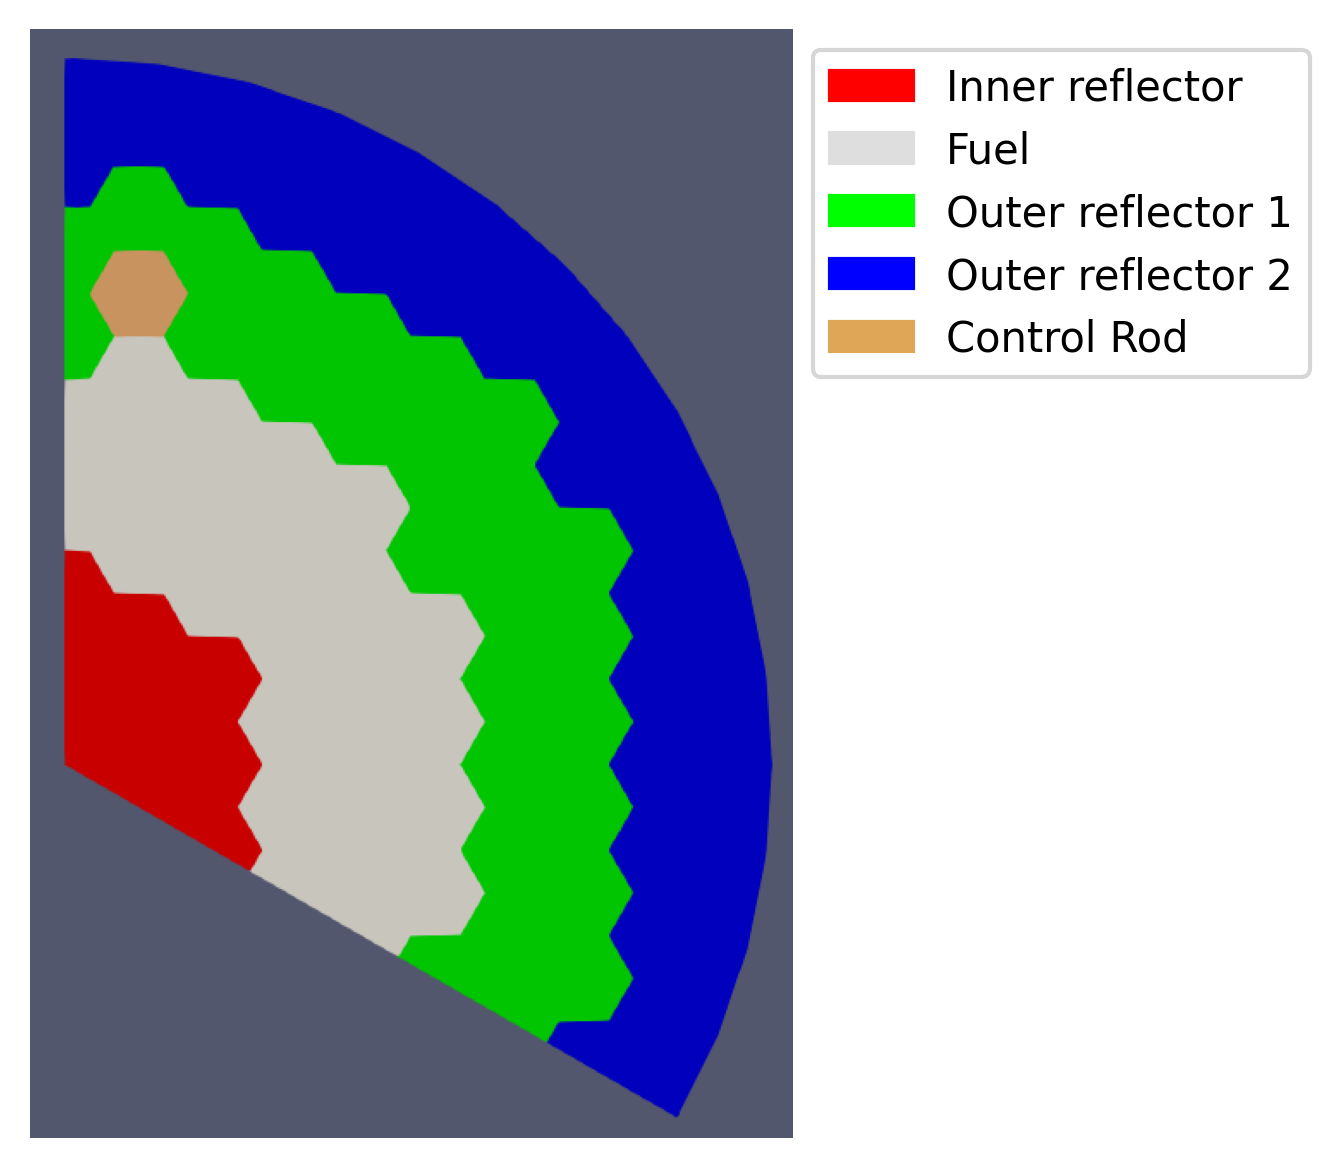
\includegraphics[width=0.6\linewidth]{figures/oecd-fullcore-legend}
	\hfill
	\caption{1/3$^{rd}$ MHTGR-350 geometry.}
	\label{fig:mesh}
\end{figure}

\begin{table}[htbp!]
  \centering
  \caption{Global parameters.}
  \begin{tabular}{l|l|l}
  \toprule
  Parameter &  Benchmark  &  Moltres    \\
  \midrule
  K$_{eff}$ &  1.06691    &  1.06804    \\
  $\Delta \rho_{CR}$ (pcm)  & 822.1 & 509.8 \\
  AO        &  0.168      &  0.1753     \\
  \bottomrule
  \end{tabular}
  \label{tab:globalparam}
\end{table}

\begin{figure}[htbp!]
  \centering
  \begin{subfigure}[t]{0.4\textwidth}
    \centering
    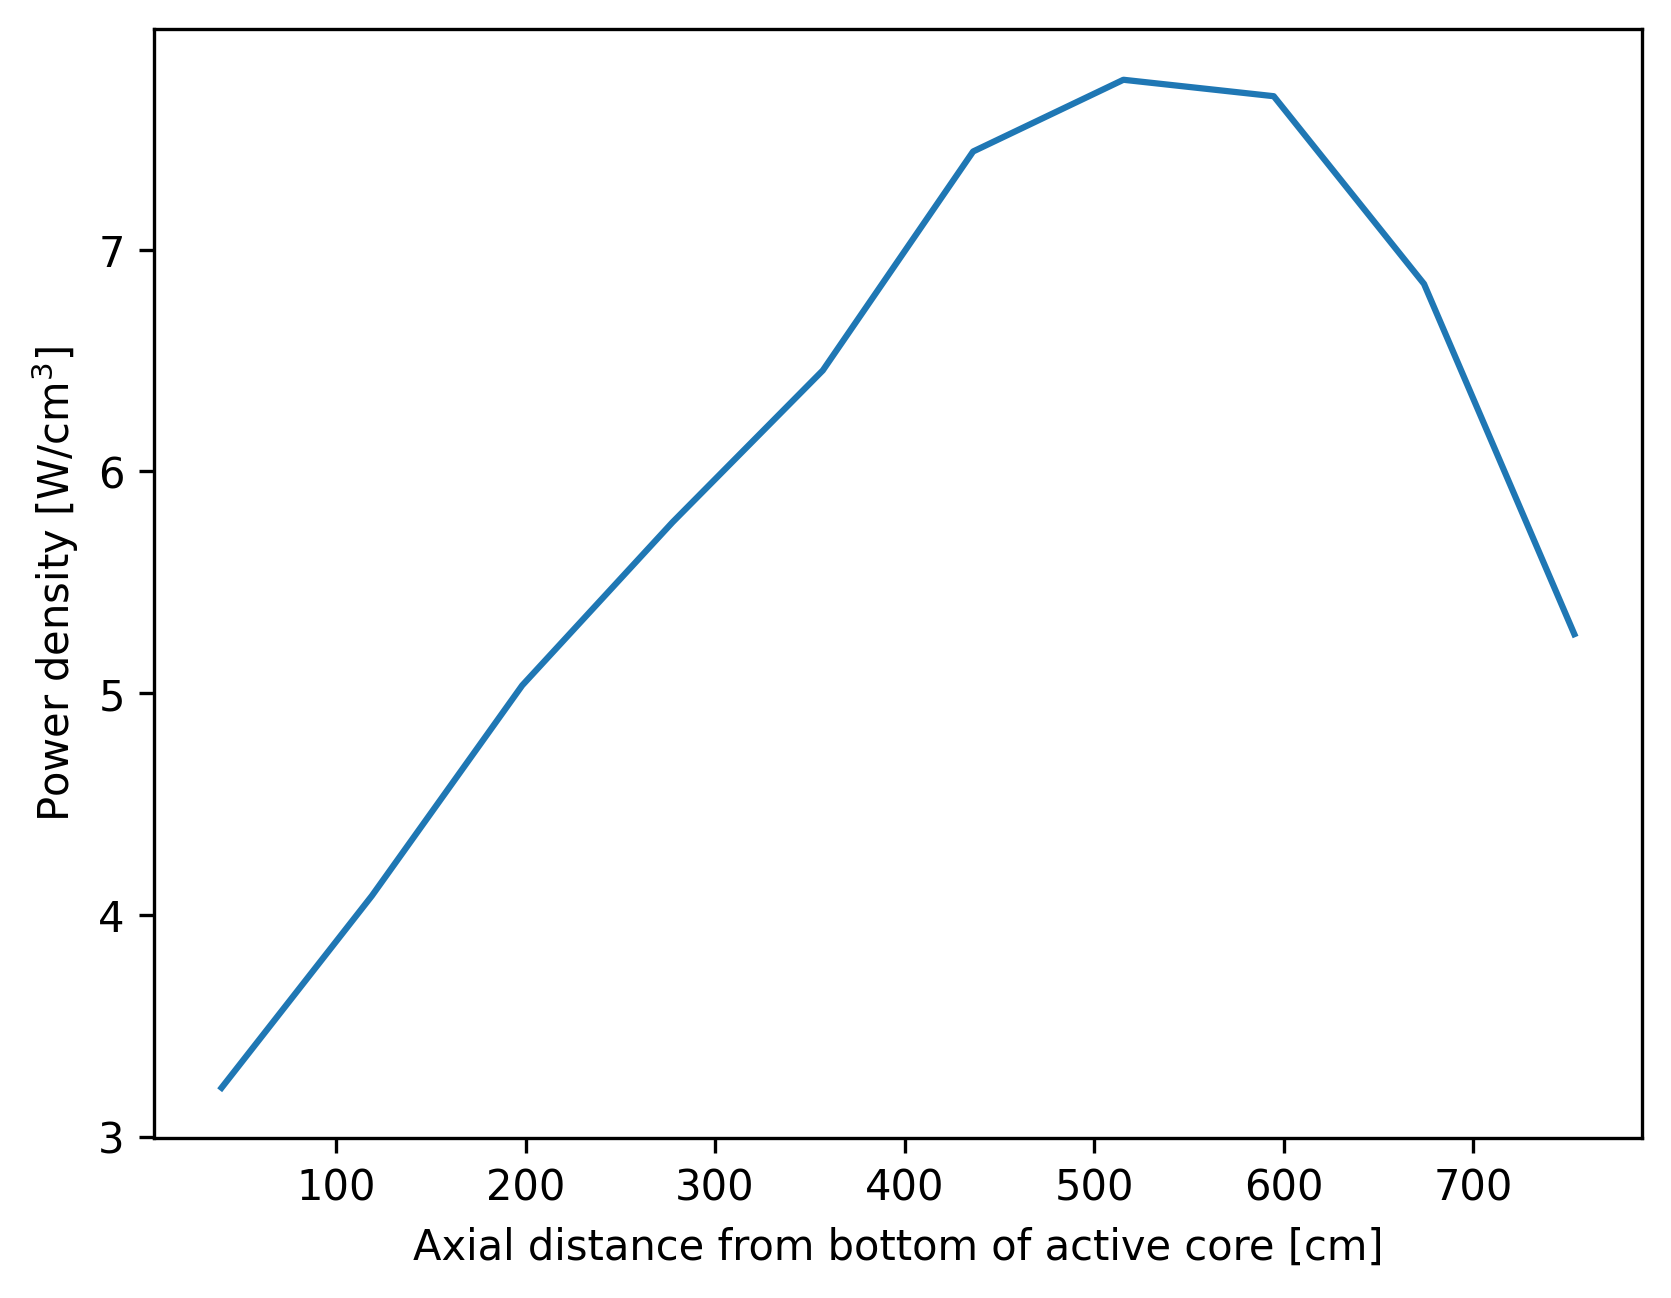
\includegraphics[height=5cm]{figures/3D-fullcore26G-axialpower}
    \caption{Moltres result.}
  \end{subfigure}
  \begin{subfigure}[t]{0.4\textwidth}
    \centering
    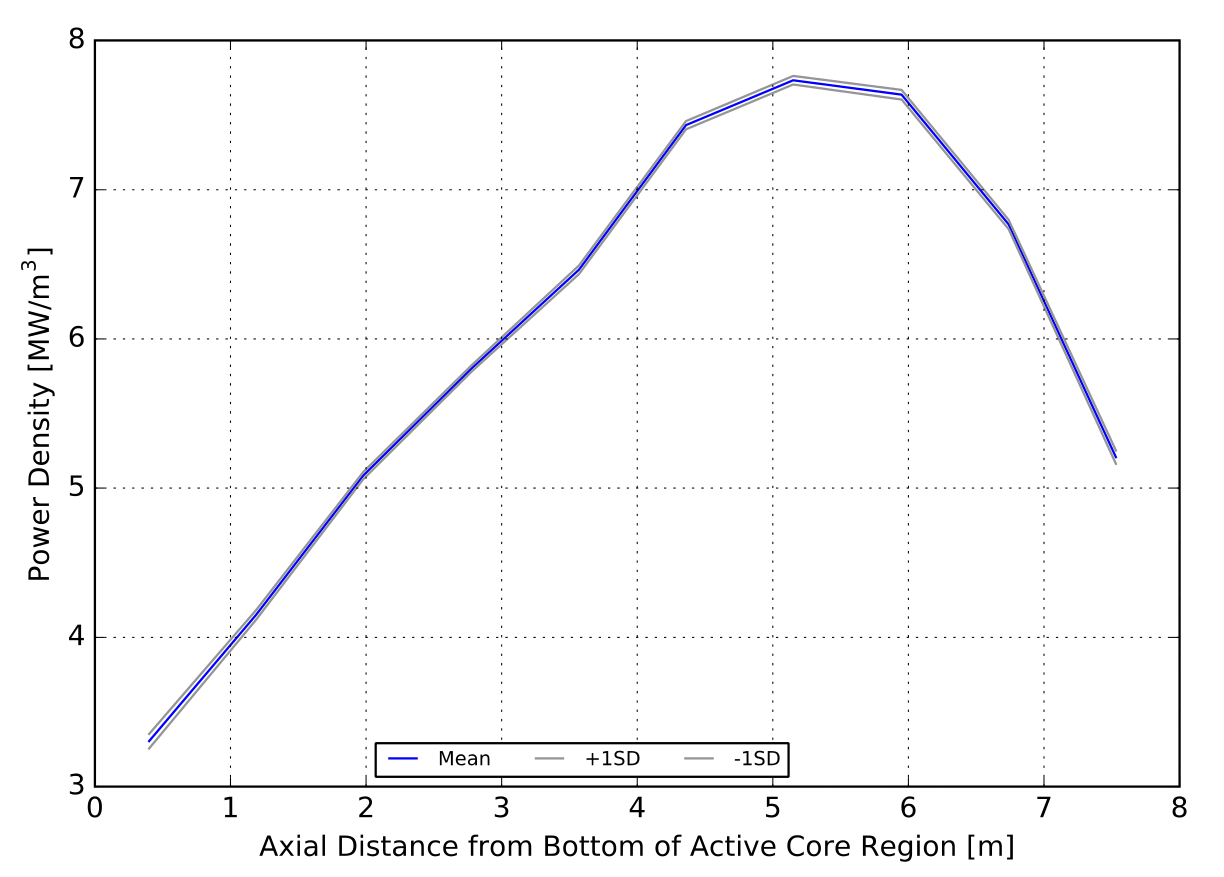
\includegraphics[height=5cm]{figures/benchmark-axialpower}
    \caption{Benchmark result. Image reproduced from \cite{oecd_nea_coupled_2020}.}
  \end{subfigure}
  \hfill
  \caption{Radially averaged axial power distribution.}
  \label{fig:axialpower}
\end{figure}

\begin{figure}[htbp!]
  \centering
  \begin{subfigure}[t]{0.4\textwidth}
    \centering
    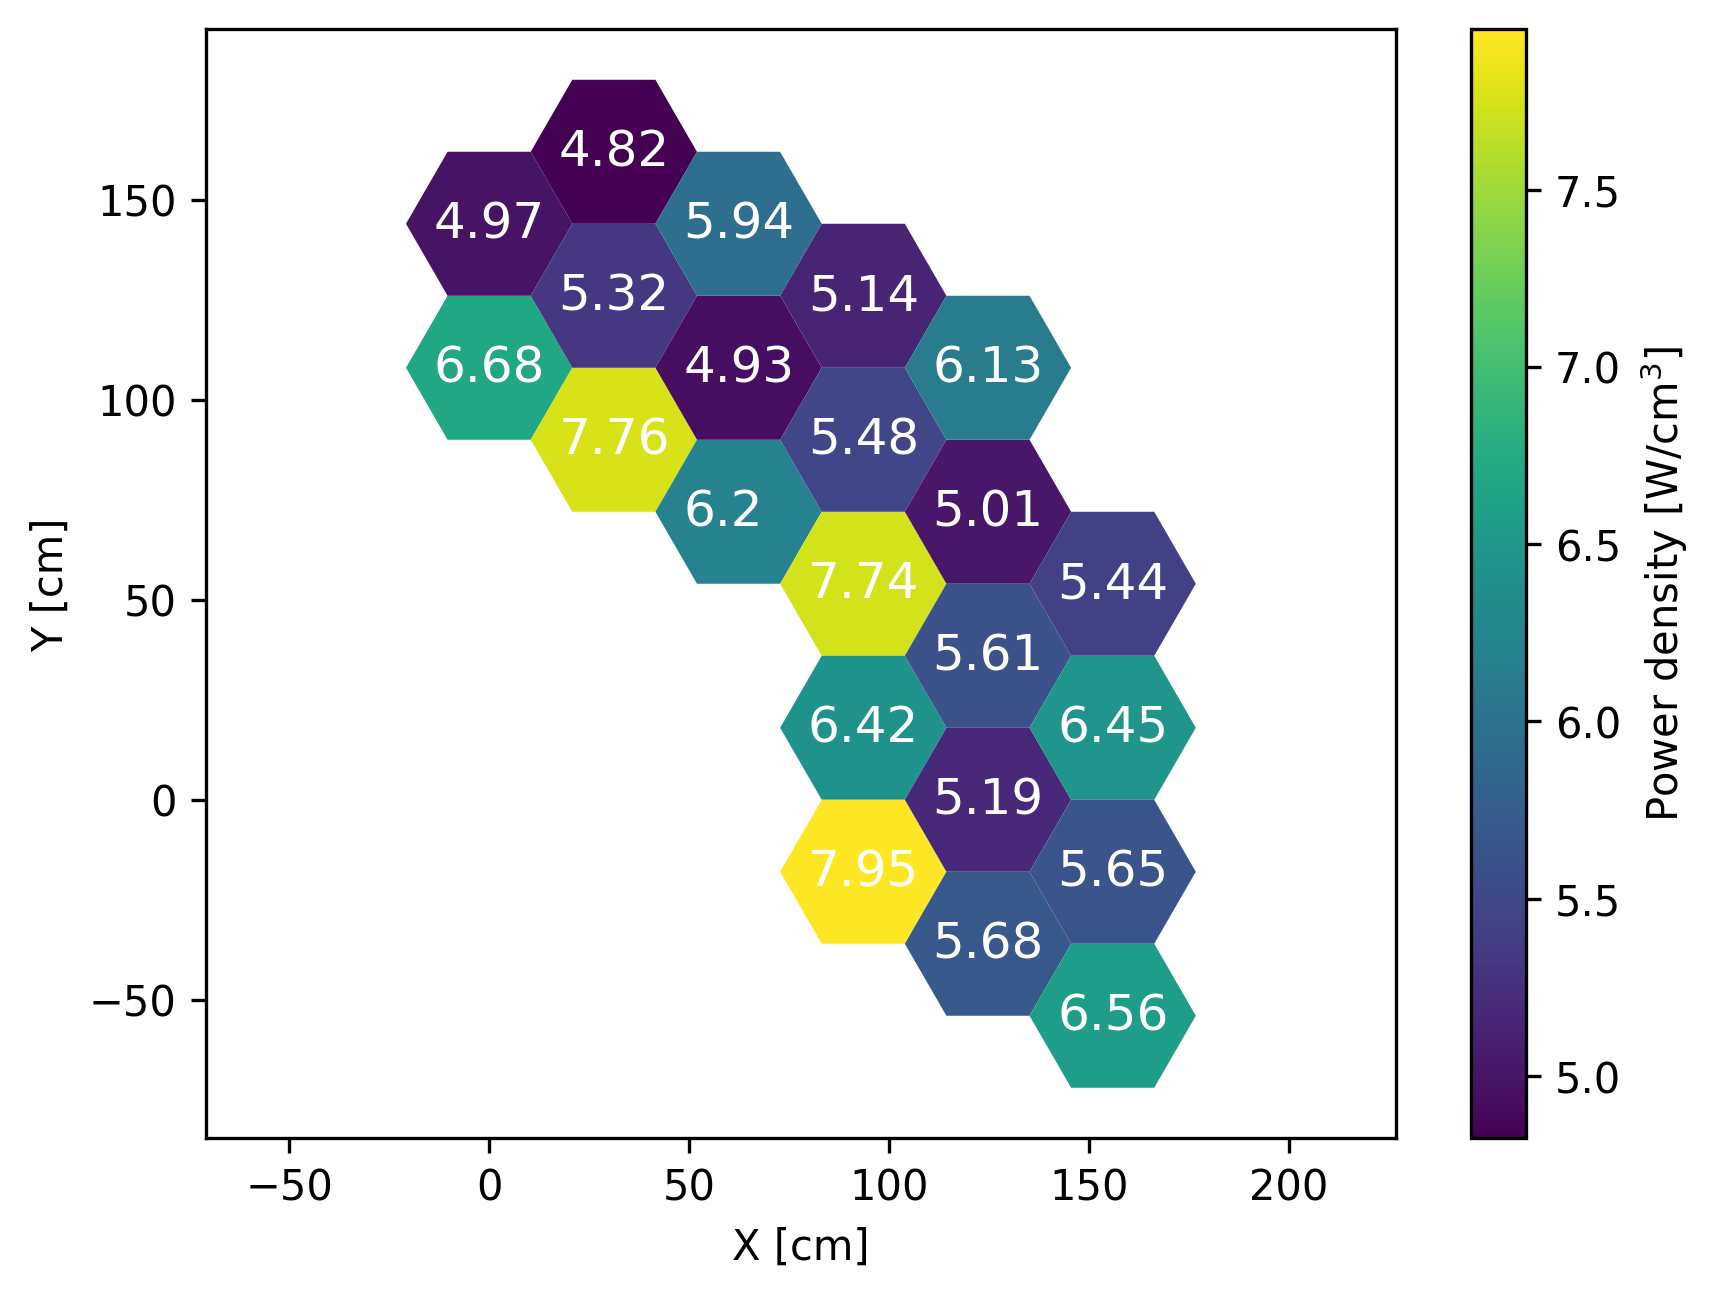
\includegraphics[width=\linewidth]{figures/3D-fullcore26G-radialpower}
    \caption{Moltres result.}
  \end{subfigure}
  \begin{subfigure}[t]{0.4\textwidth}
    \centering
    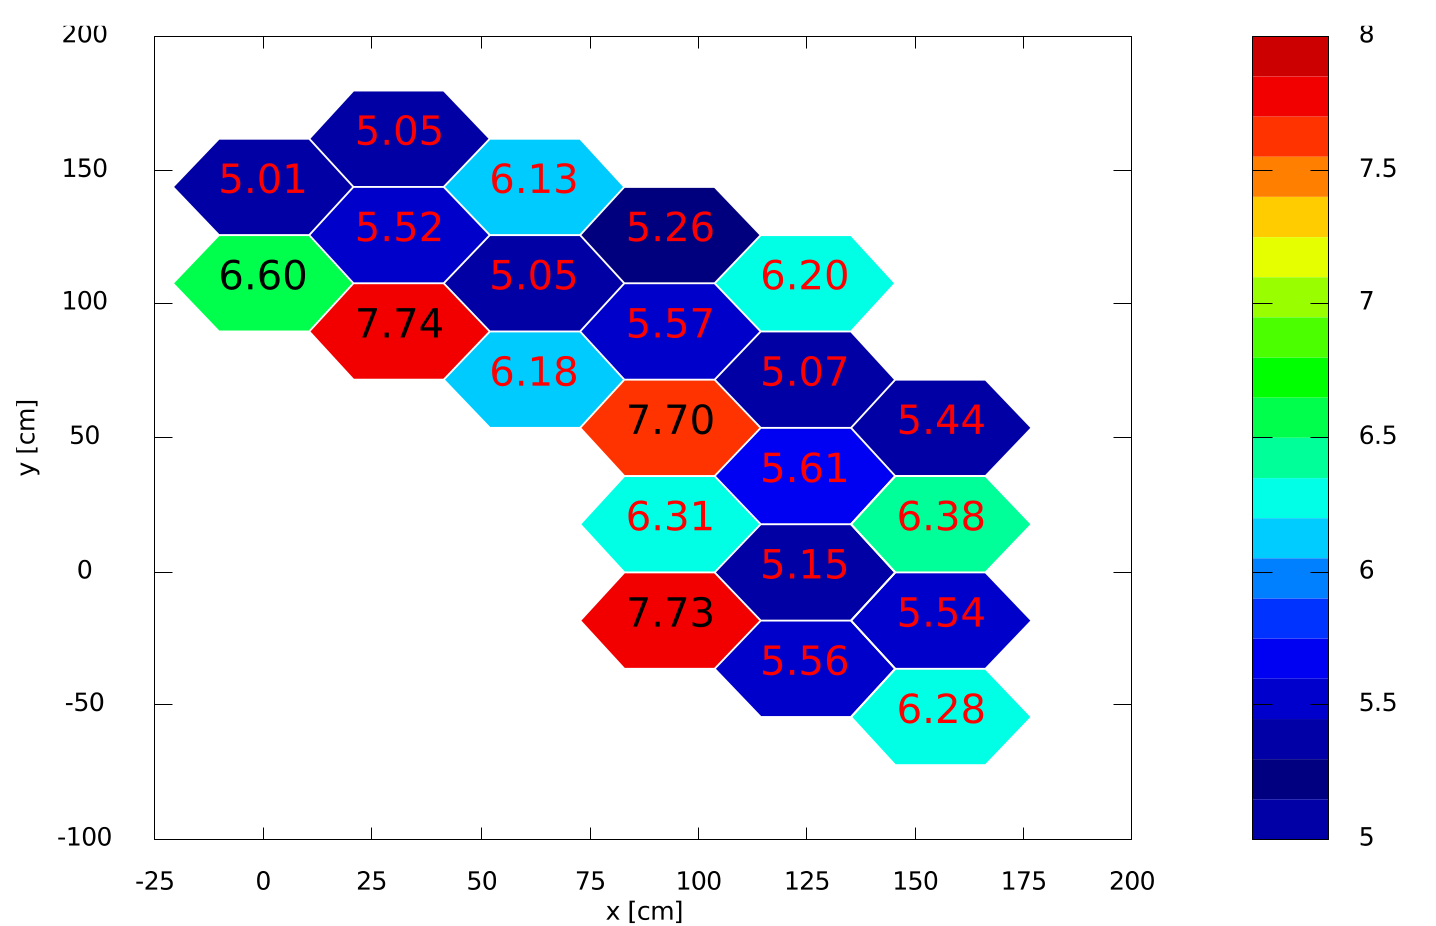
\includegraphics[width=\linewidth]{figures/benchmark-radialpower}
    \caption{Benchmark result. Image reproduced from \cite{oecd_nea_coupled_2020}.}
  \end{subfigure}
  \hfill
  \caption{Axially averaged radial power distribution.}
  \label{fig:radialpower}
\end{figure}

\subsection{Periodic vs Neumann BCs}

Table \ref{tab:benchmark-bc}

3G)
62118 dofs/group = 186354 dofs

6G)
16898 dofs/group = 101388 dofs

\begin{table}[htbp!]
  \centering
  \caption{Global parameters comparison for different types of BCs.}
  \begin{tabular}{l|l|l|l|l|l}
  \toprule
  Energy groups       & Type of BCs & K$_{eff, out}$ & K$_{eff, in}$ & $\Delta \rho_{CR}$ (pcm) & AO \\
  \midrule
  \multirow{2}{*}{3}  & Periodic    & 1.07571		& 1.06776		& 692.6		& 0.237		\\
                      & Neumann     & 1.07586	  & 1.07021   & 490.5		& 0.237	  \\ \hline
  \multirow{2}{*}{6}  & Periodic    & 1.07182		& 1.06356		& 724.3	  & 0.185  	\\
                      & Neumann     & 1.07197   & 1.06610 	& 513.3		& 0.186		\\  
  \bottomrule
  \end{tabular}
  \label{tab:benchmark-bc}
\end{table}



\section{Assembly}

Moltres DOFs: 
N of elements: 37120
Nodes (DOFs/group): 22862

Serpent Keff:
noLBP-600: 1.43800
noLBP-1200: 1.37771
LBP-600: 1.12861
LBP-1200: 1.06554

Table \ref{tab:energygroups}

Figure \ref{fig:assembly-noLBP-600-flux}
Figure \ref{fig:assembly-noLBP-600}

Figure \ref{fig:assembly-noLBP-1200-flux}
Figure \ref{fig:assembly-noLBP-1200}

Figure \ref{fig:assembly-LBP-600-flux}
Figure \ref{fig:assembly-LBP-600}

Figure \ref{fig:assembly-LBP-1200-flux}
Figure \ref{fig:assembly-LBP-1200}

Figure \ref{fig:assembly-time}

Table \ref{tab:accuracy15}

\begin{figure}[htbp!]
	\centering
	\begin{subfigure}[t]{0.4\textwidth}
		\centering
		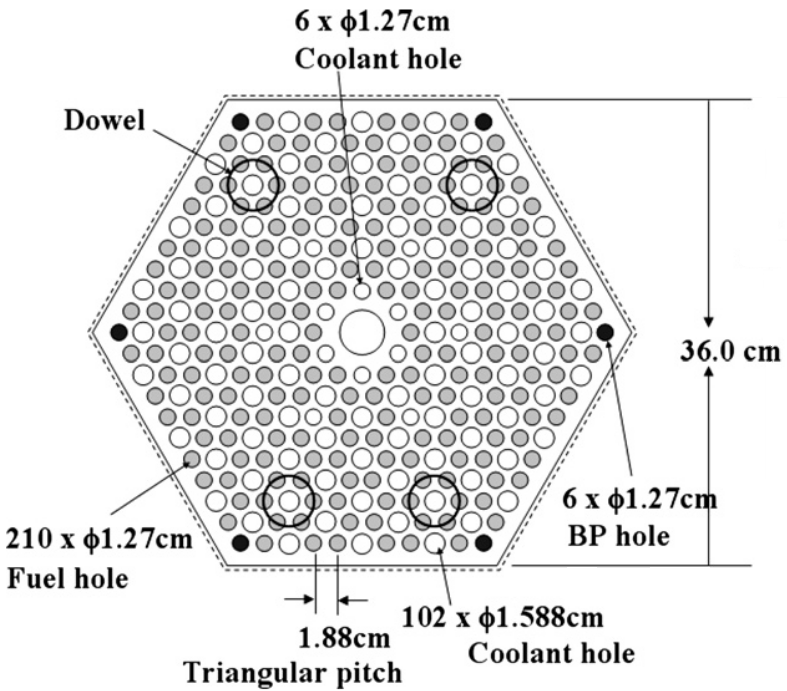
\includegraphics[width=\linewidth]{figures/fuel-assembly}
		\caption{Fuel column geometry. Image reproduced form \cite{tak_numerical_2008}.}
	\end{subfigure}
	\begin{subfigure}[t]{0.4\textwidth}
		\centering
		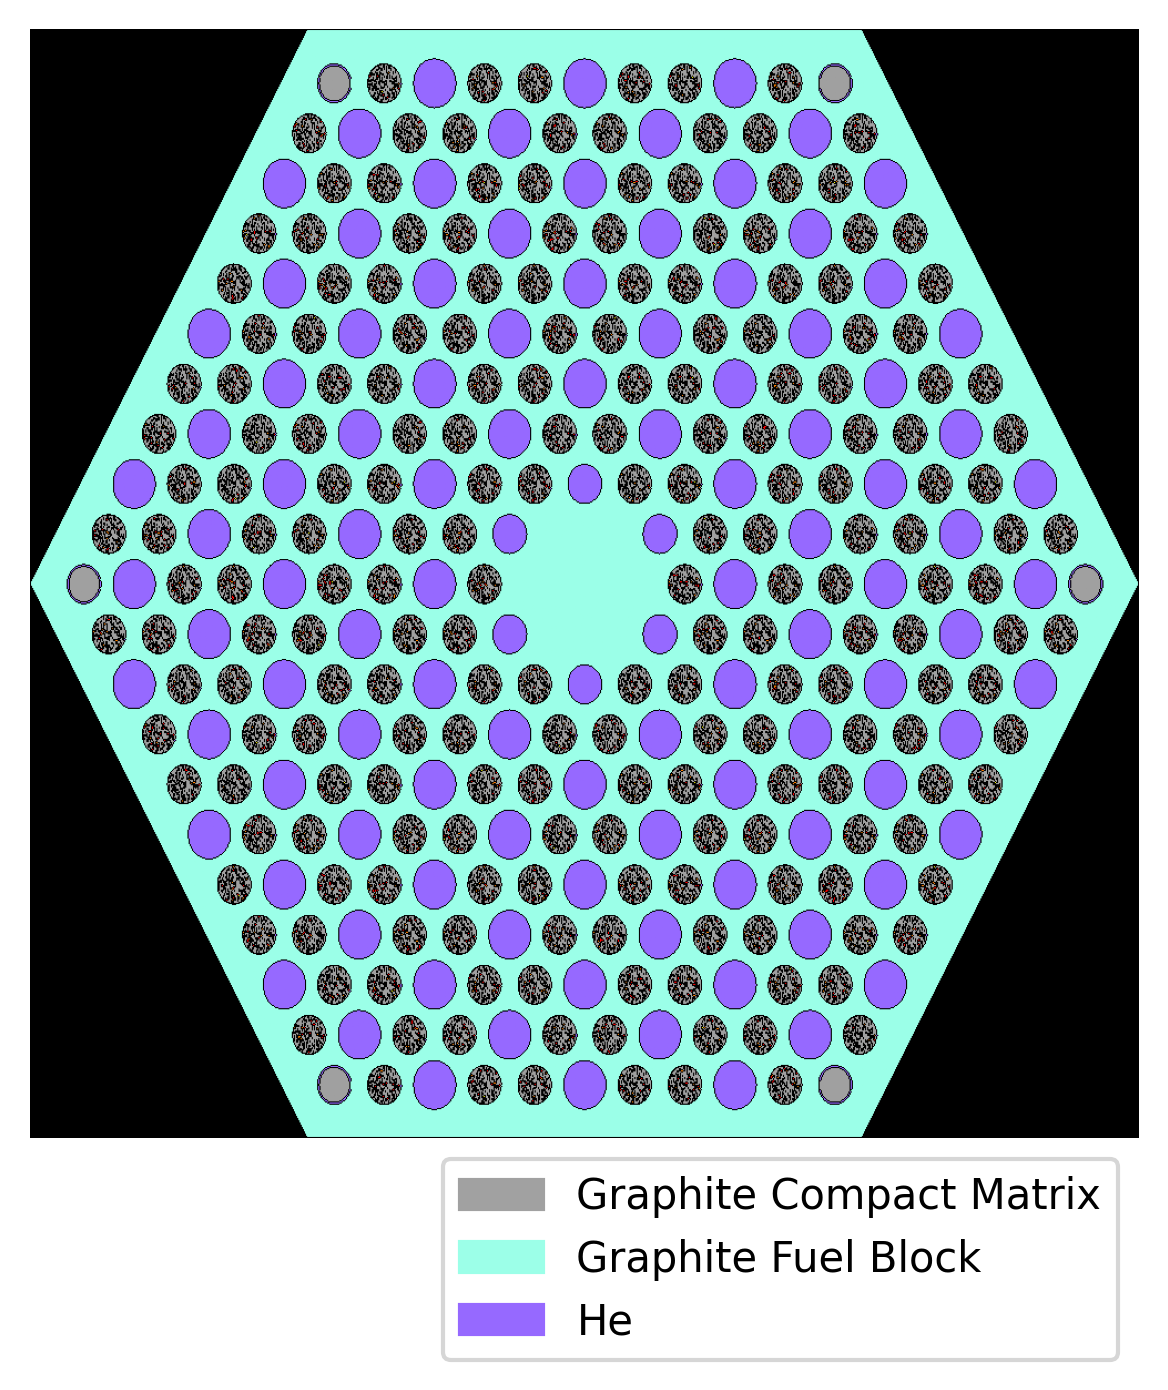
\includegraphics[width=\linewidth]{figures/oecd-standard-column-legend}
		\caption{Serpent model geometry.}
	\end{subfigure}
	\hfill
	\caption{Fuel column of the MHTGR-350. XY-plane in the active core region.}
	\label{fig:}
\end{figure}

\begin{table}[htbp!]
  \centering
  \caption{Energy group structure.}
  \begin{tabular}{c|l|l|l|l|l|l|l|l|l|l|l|l}
  \toprule
  Upper boundary [eV] & 26    & 21   & 18   & 15a & 15b & 15c & 15d & 15e   & 12  & 9  & 6  & 3 \\
  \midrule
  1.49E+07            & 1     & 1    & 1    & 1   & 1   & 1   & 1   & 1     & 1   & 1  & 1  & 1 \\ \cline{1-2}
  7.41E+06            & 2     &      &      &     &     &     &     &       &     &    &    &   \\ \cline{1-10}
  3.68E+06            & 3     & 2    & 2    & 2   & 2   & 2   & 2   & 2     & 2   &    &    &   \\ \cline{1-2}
  6.72E+05            & 4     &      &      &     &     &     &     &       &     &    &    &   \\ \hline
  1.11E+05            & 5     & 3    & 3    & 3   & 3   & 3   & 3   & 3     & 3   & 2  & 2  & 2 \\ \cline{1-6} \cline{10-10}
  1.93E+04            & 6     & 4    & 4    & 4   & 4   &     &     &       & 4   &    &    &   \\ \cline{1-2}
  3.35E+03            & 7     &      &      &     &     &     &     &       &     &    &    &   \\ \cline{1-4} \cline{7-7}
  1.58E+03            & 8     & 5    & 5    &     &     & 4   &     &       &     &    &    &   \\ \cline{1-6} \cline{8-11}
  7.48E+02            & 9     & 6    & 6    & 5   & 5   &     & 4   & 4     & 5   & 3  &    &   \\ \cline{1-7} \cline{10-11}
  2.75E+02            & 10    & 7    & 7    & 6   & 6   & 5   &     &       & 6   & 4  &    &   \\ \cline{1-6} \cline{8-12}
  1.30E+02            & 11    & 8    & 8    & 7   & 7   &     & 5   & 5     & 7   & 5  & 3  &   \\ \cline{1-3} \cline{6-7}
  6.14E+01            & 12    & 9    &      &     & 8   & 6   &     &       &     &    &    &   \\ \cline{1-6} \cline{8-9}
  2.90E+01            & 13    & 10   & 9    & 8   & 9   &     & 6   & 6     &     &    &    &   \\ \cline{1-5} \cline{10-11}
  1.37E+01            & 14    & 11   & 10   & 9   &     &     &     &       & 8   & 6  &    &   \\ \cline{1-10}
  8.32E+00            & 15    & 12   & 11   & 10  & 10  & 7   & 7   & 7     & 9   &    &    &   \\ \cline{1-2}
  5.04E+00            & 16    &      &      &     &     &     &     &       &     &    &    &   \\ \hline
  2.38E+00            & 17    & 13   & 12   & 11  & 11  & 8   & 8   & 8     & 10  & 7  & 4  & 3 \\ \cline{1-3}
  1.29E+00            & 18    & 14   &      &     &     &     &     &       &     &    &    &   \\ \cline{1-12} 
  6.50E-01            & 19    & 15   & 13   & 12  & 12  & 9   & 9   & 9     & 11  & 8  & 5  &   \\ \cline{1-3} \cline{7-8}
  3.50E-01            & 20    & 16   &      &     &     & 10  & 10  &       &     &    &    &   \\ \cline{1-9}
  2.00E-01            & 21    & 17   & 14   & 13  & 13  & 11  & 11  & 10    &     &    &    &   \\ \cline{1-2} \cline{9-9}
  1.20E-01            & 22    &      &      &     &     &     &     & 11    &     &    &    &   \\ \cline{1-9} 
  8.00E-02            & 23    & 18   & 15   & 14  & 14  & 12  & 12  & 12    &     &    &    &   \\ \cline{1-4} \cline{7-9}
  5.00E-02            & 24    & 19   & 16   &     &     & 13  & 13  & 13    &     &    &    &   \\ \hline
  2.00E-02            & 25    & 20   & 17   & 15  & 15  & 14  & 14  & 14    & 12  & 9  & 6  &   \\ \cline{1-4} \cline{7-9}
  1.00E-02            & 26    & 21   & 18   &     &     & 15  & 15  & 15    &     &    &    &   \\
  \bottomrule
  \end{tabular}
  \label{tab:energygroups}
\end{table}

% No LBP 600
\begin{figure}[htbp!]
	\centering
	\begin{subfigure}[t]{0.4\textwidth}
		\centering
		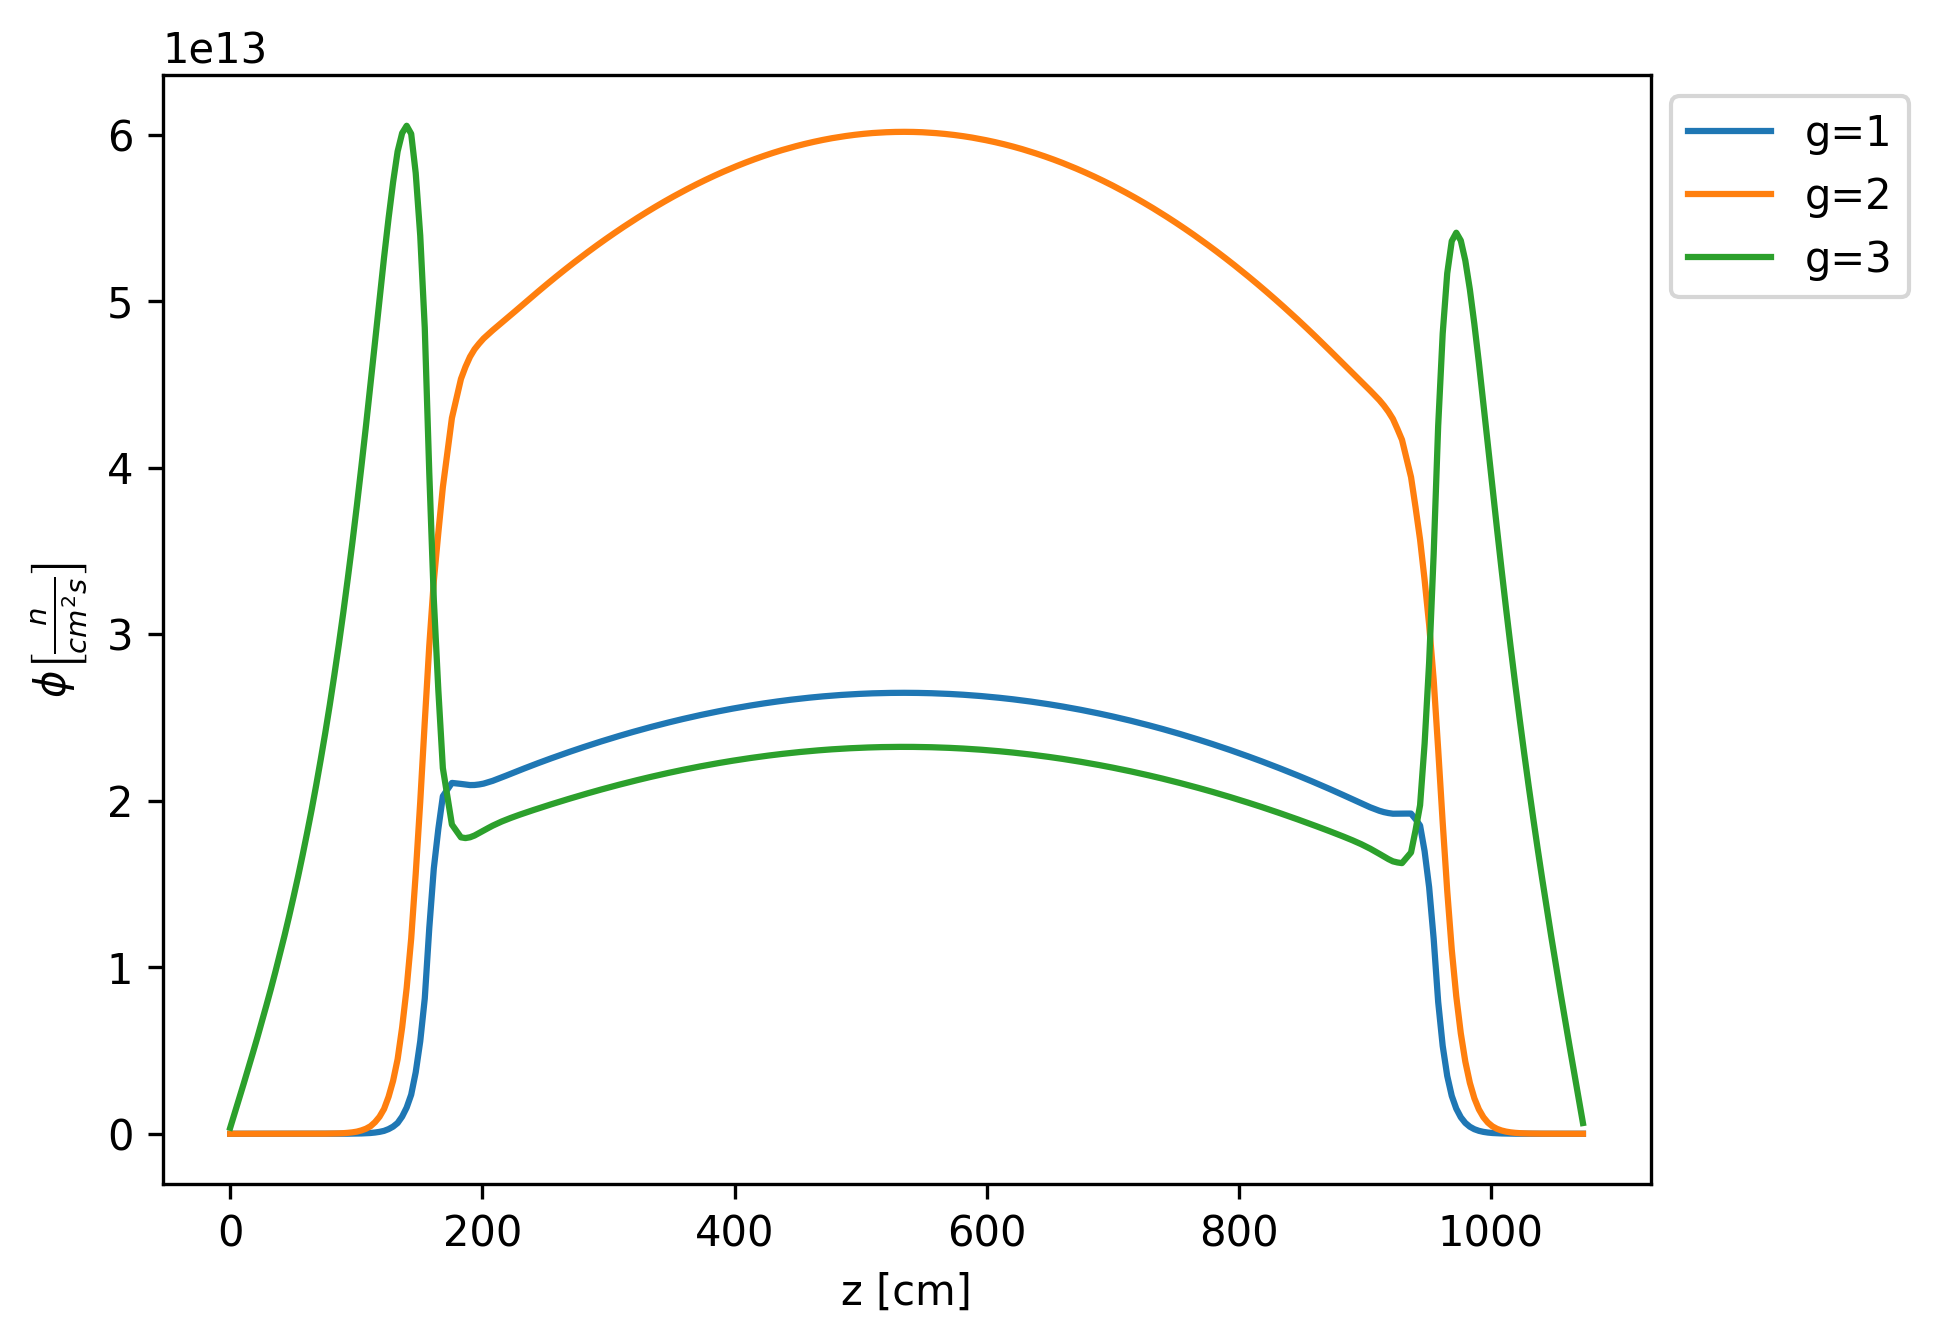
\includegraphics[width=\linewidth]{figures/3D-assembly-noLBP-600-26G}
		\caption{Moltres.}
	\end{subfigure}
	\begin{subfigure}[t]{0.4\textwidth}
		\centering
		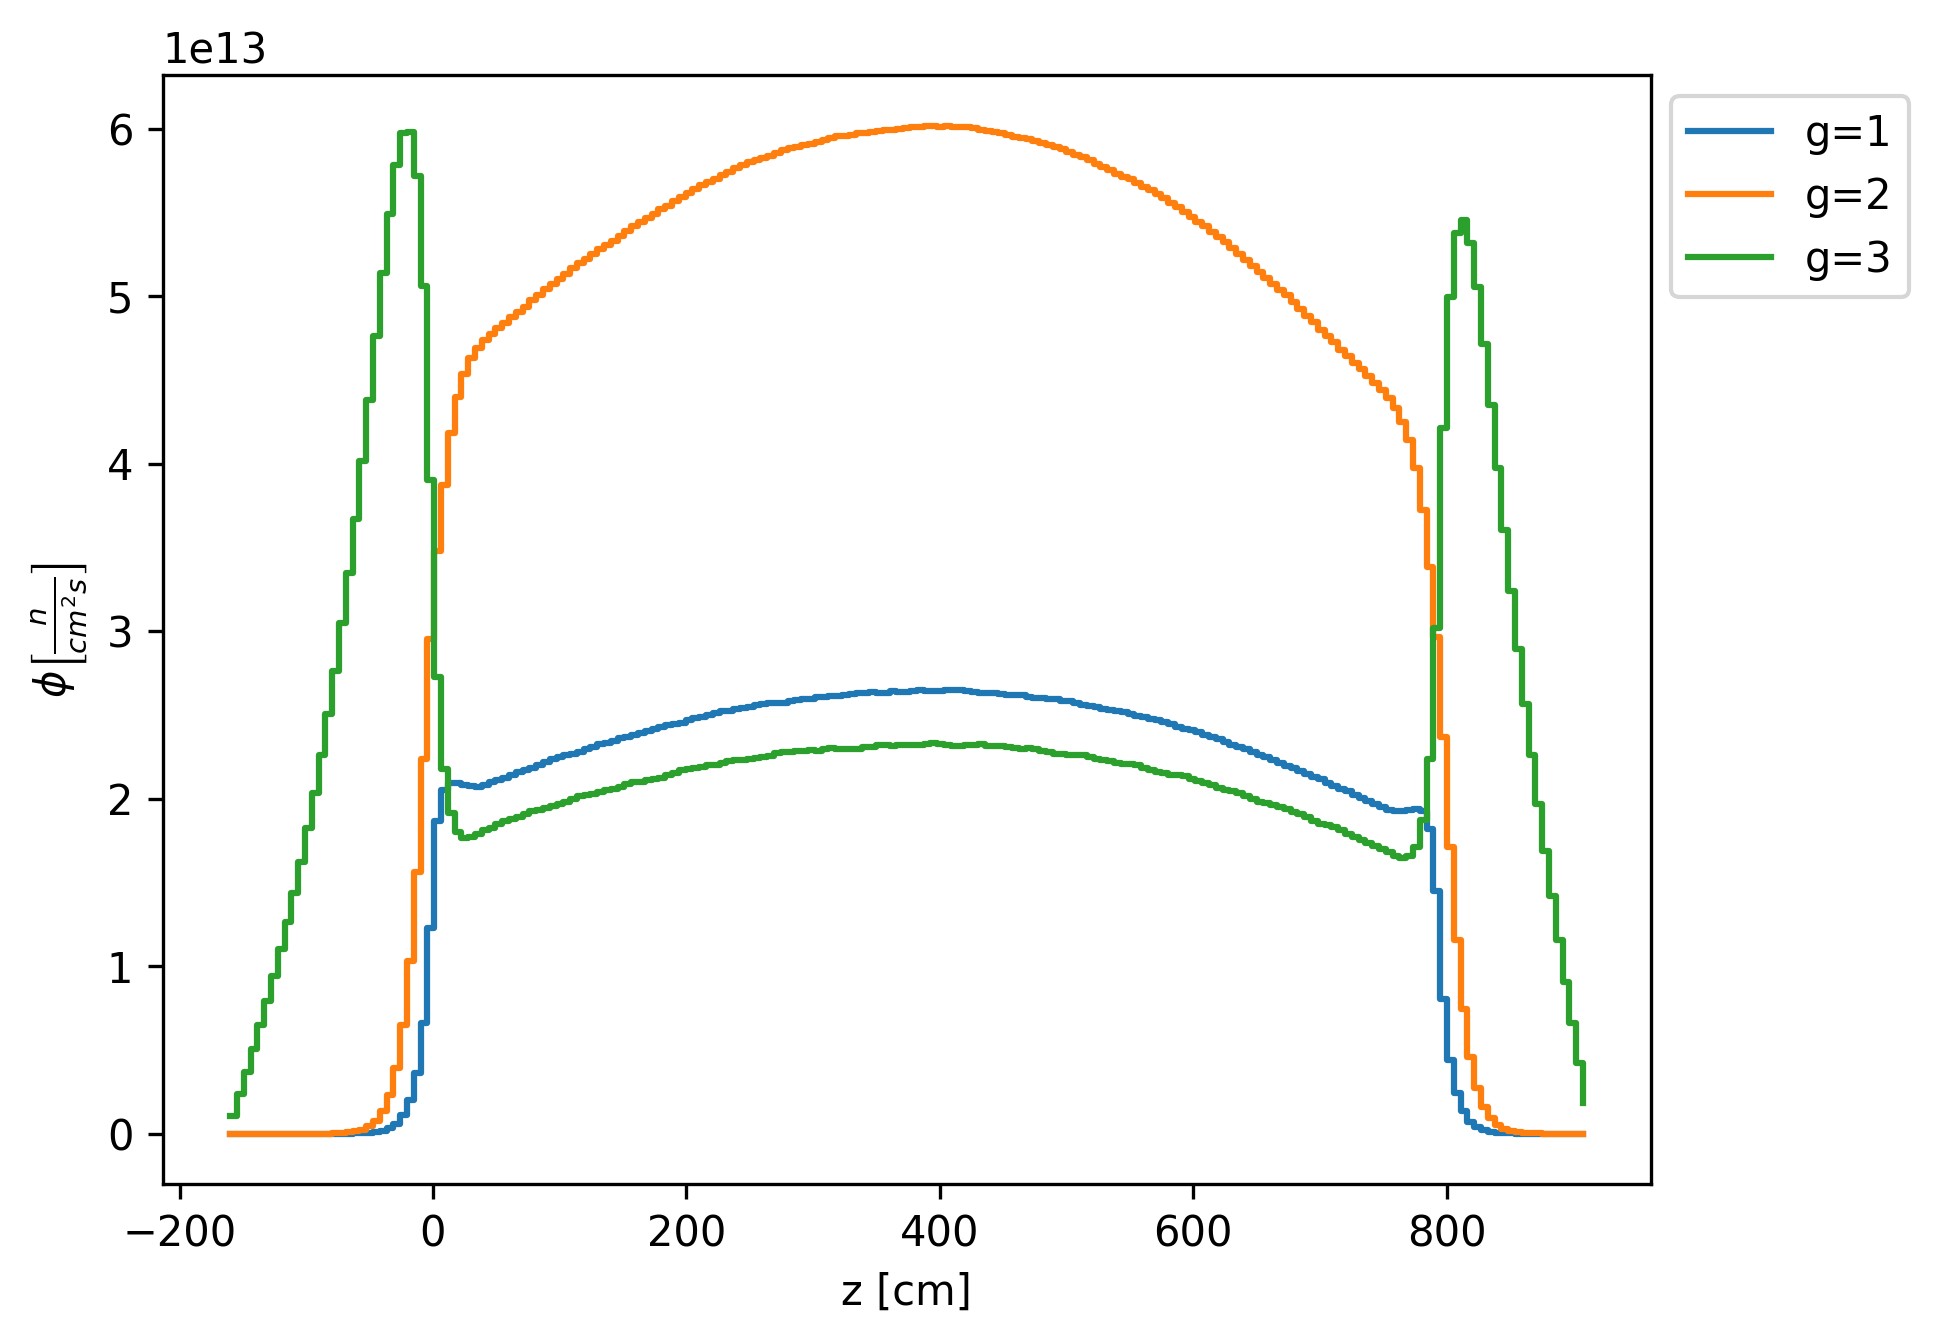
\includegraphics[width=\linewidth]{figures/serpent26G-noLBP-600-collapse}
		\caption{Serpent.}
	\end{subfigure}
	\hfill
	\caption{Axial neutron flux for 3 groups.}
	\label{fig:assembly-noLBP-600-flux}
\end{figure}

\begin{figure}[htbp!]
	\centering
	\begin{subfigure}[t]{0.4\textwidth}
		\centering
		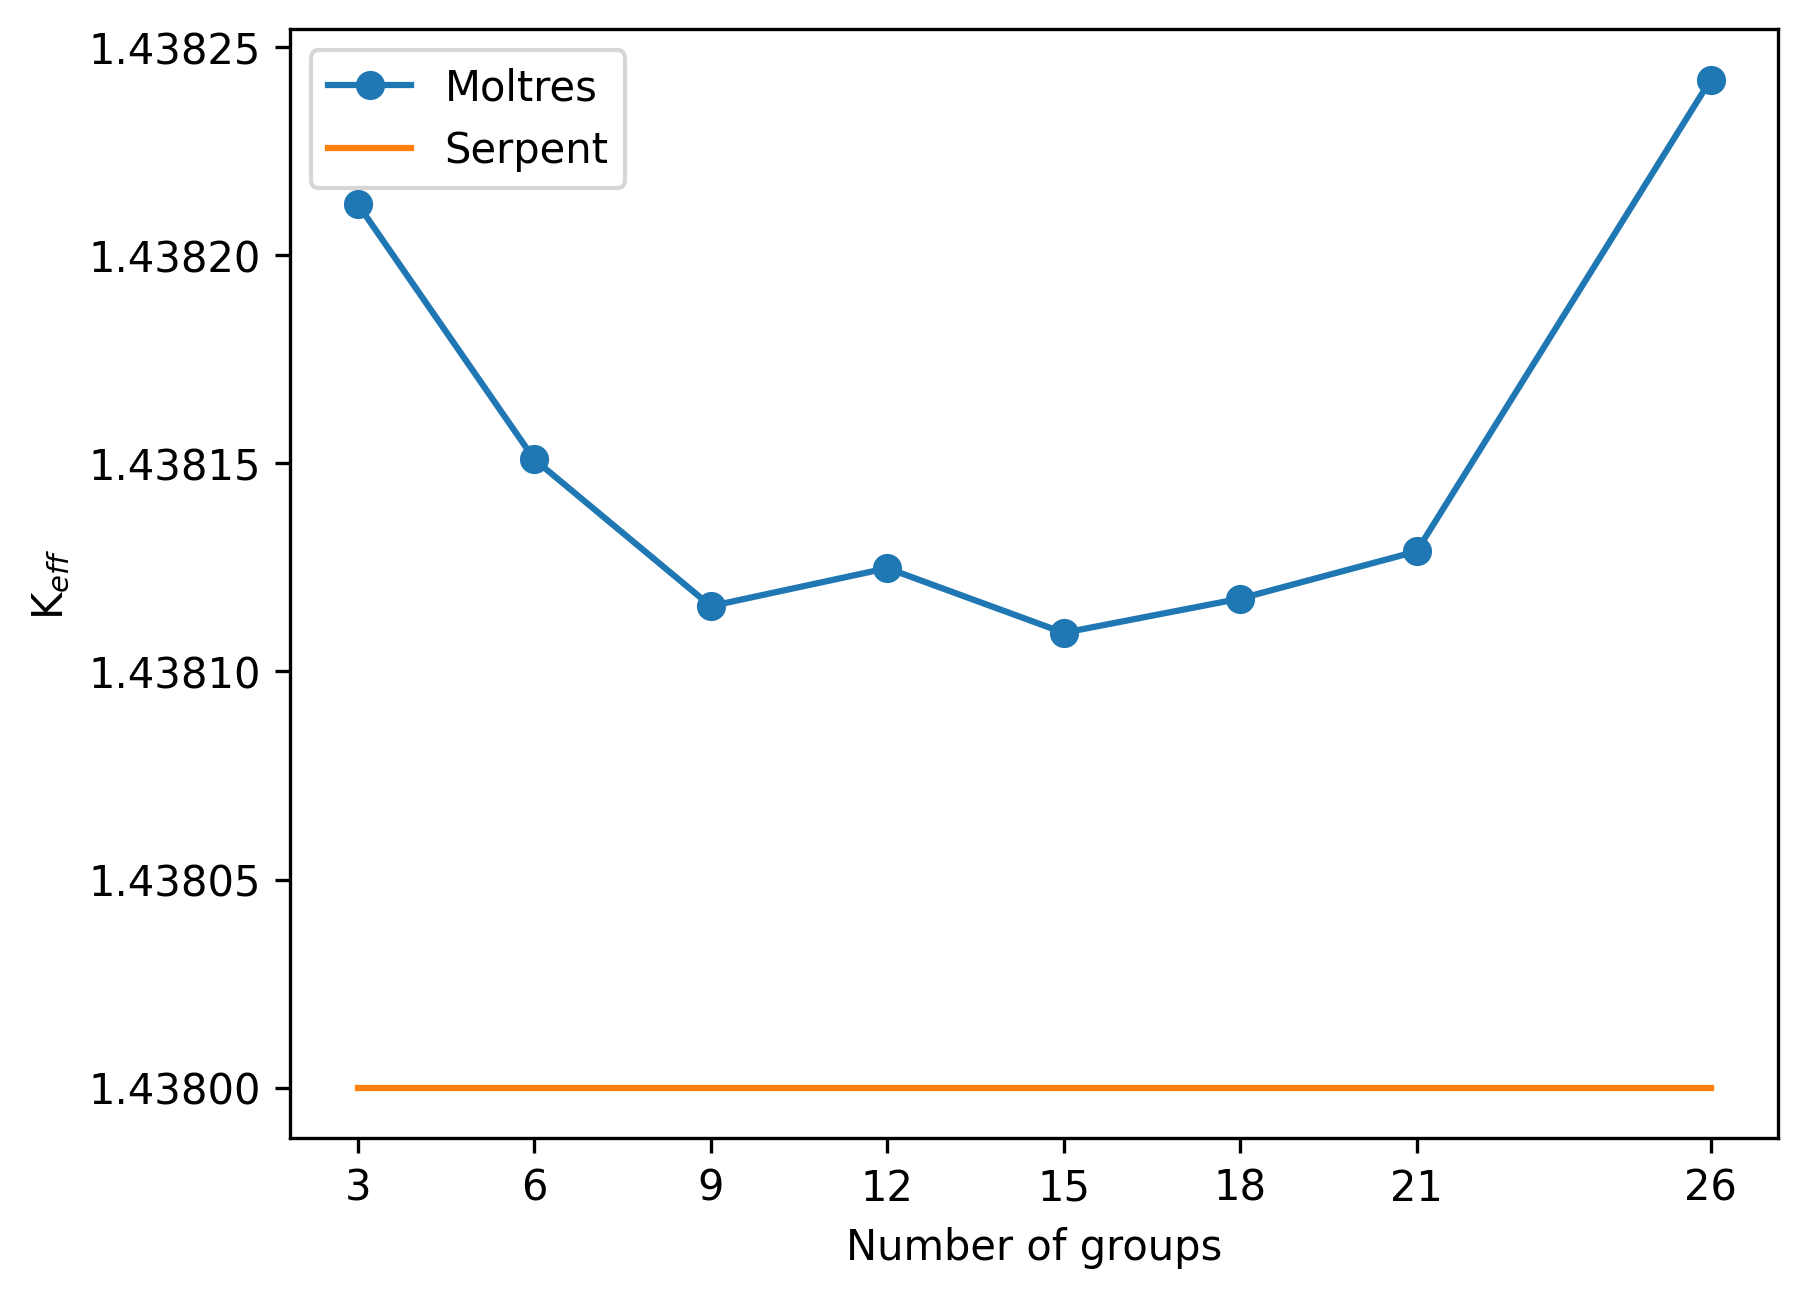
\includegraphics[width=\linewidth]{figures/keff-noLBP-600}
		\caption{Multiplication factor.}
	\end{subfigure}
	\begin{subfigure}[t]{0.4\textwidth}
		\centering
		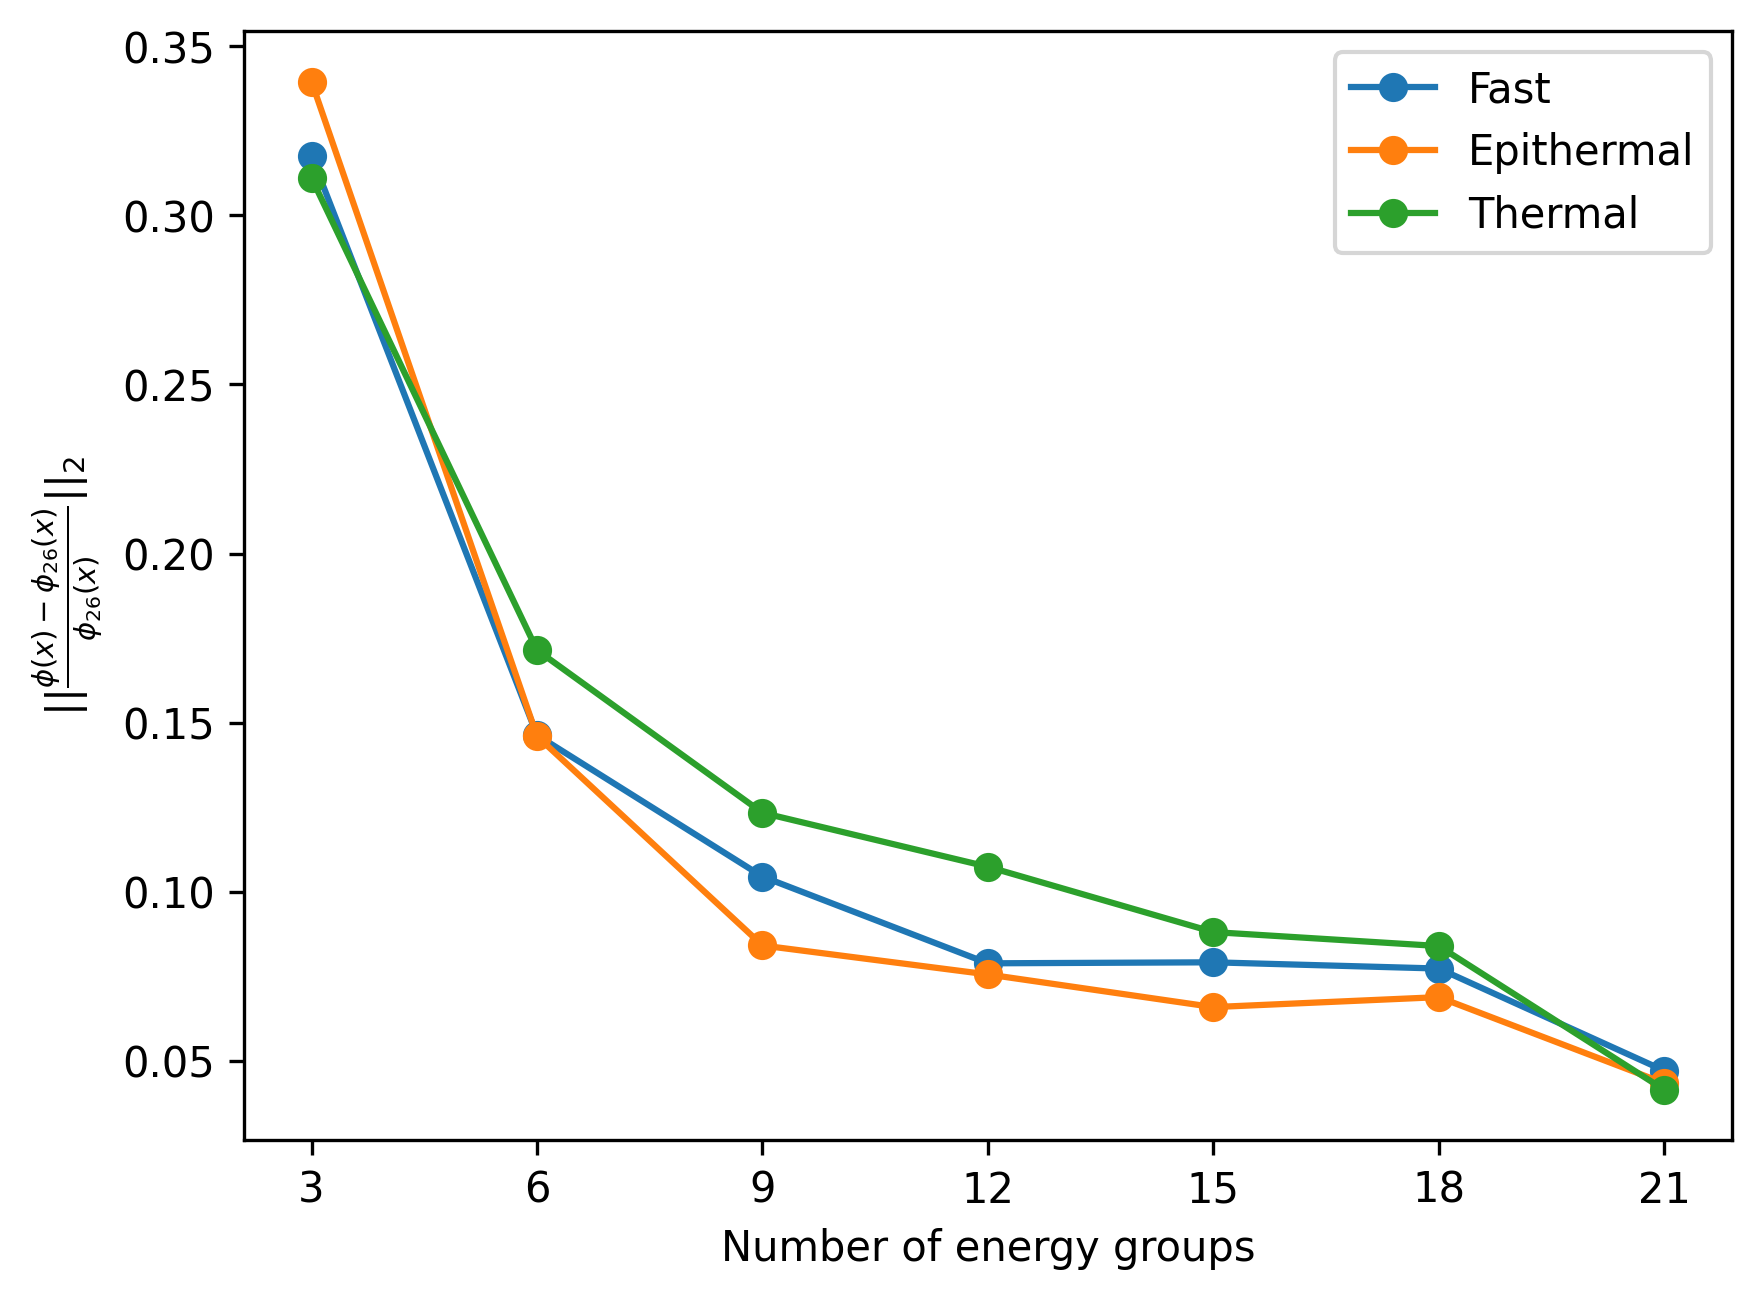
\includegraphics[width=\linewidth]{figures/noLBP-600-er-final}
		\caption{L$_2$-norm relative error.}
	\end{subfigure}
	\hfill
	\caption{Effect of different number of energy group structures over different parameters.}
	\label{fig:assembly-noLBP-600}
\end{figure}

% No LBP 1200
\begin{figure}[htbp!]
	\centering
	\begin{subfigure}[t]{0.4\textwidth}
		\centering
		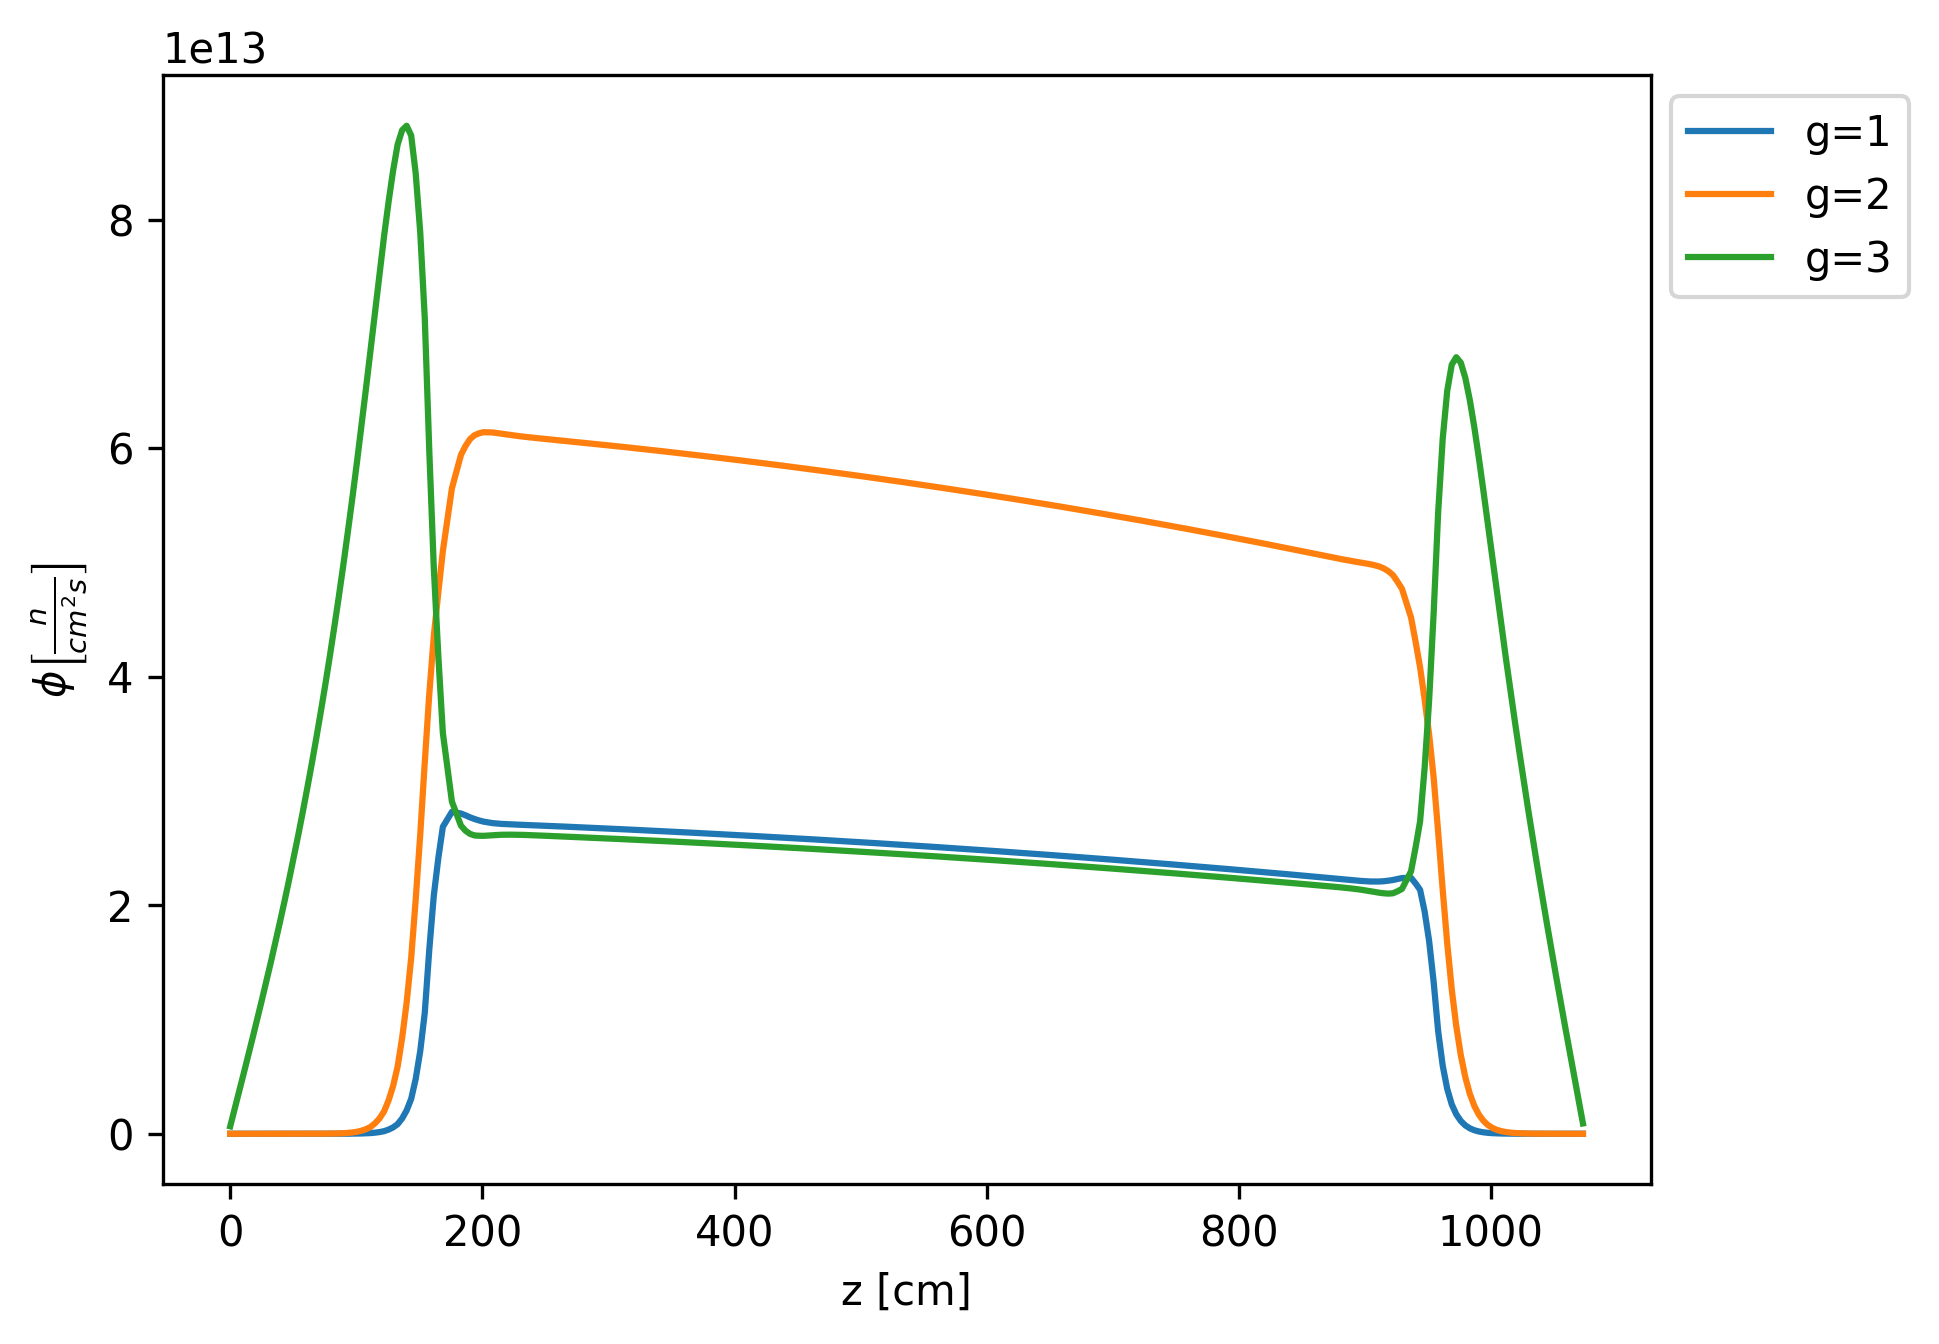
\includegraphics[width=\linewidth]{figures/3D-assembly-noLBP-1200-26G}
		\caption{Moltres.}
	\end{subfigure}
	\begin{subfigure}[t]{0.4\textwidth}
		\centering
		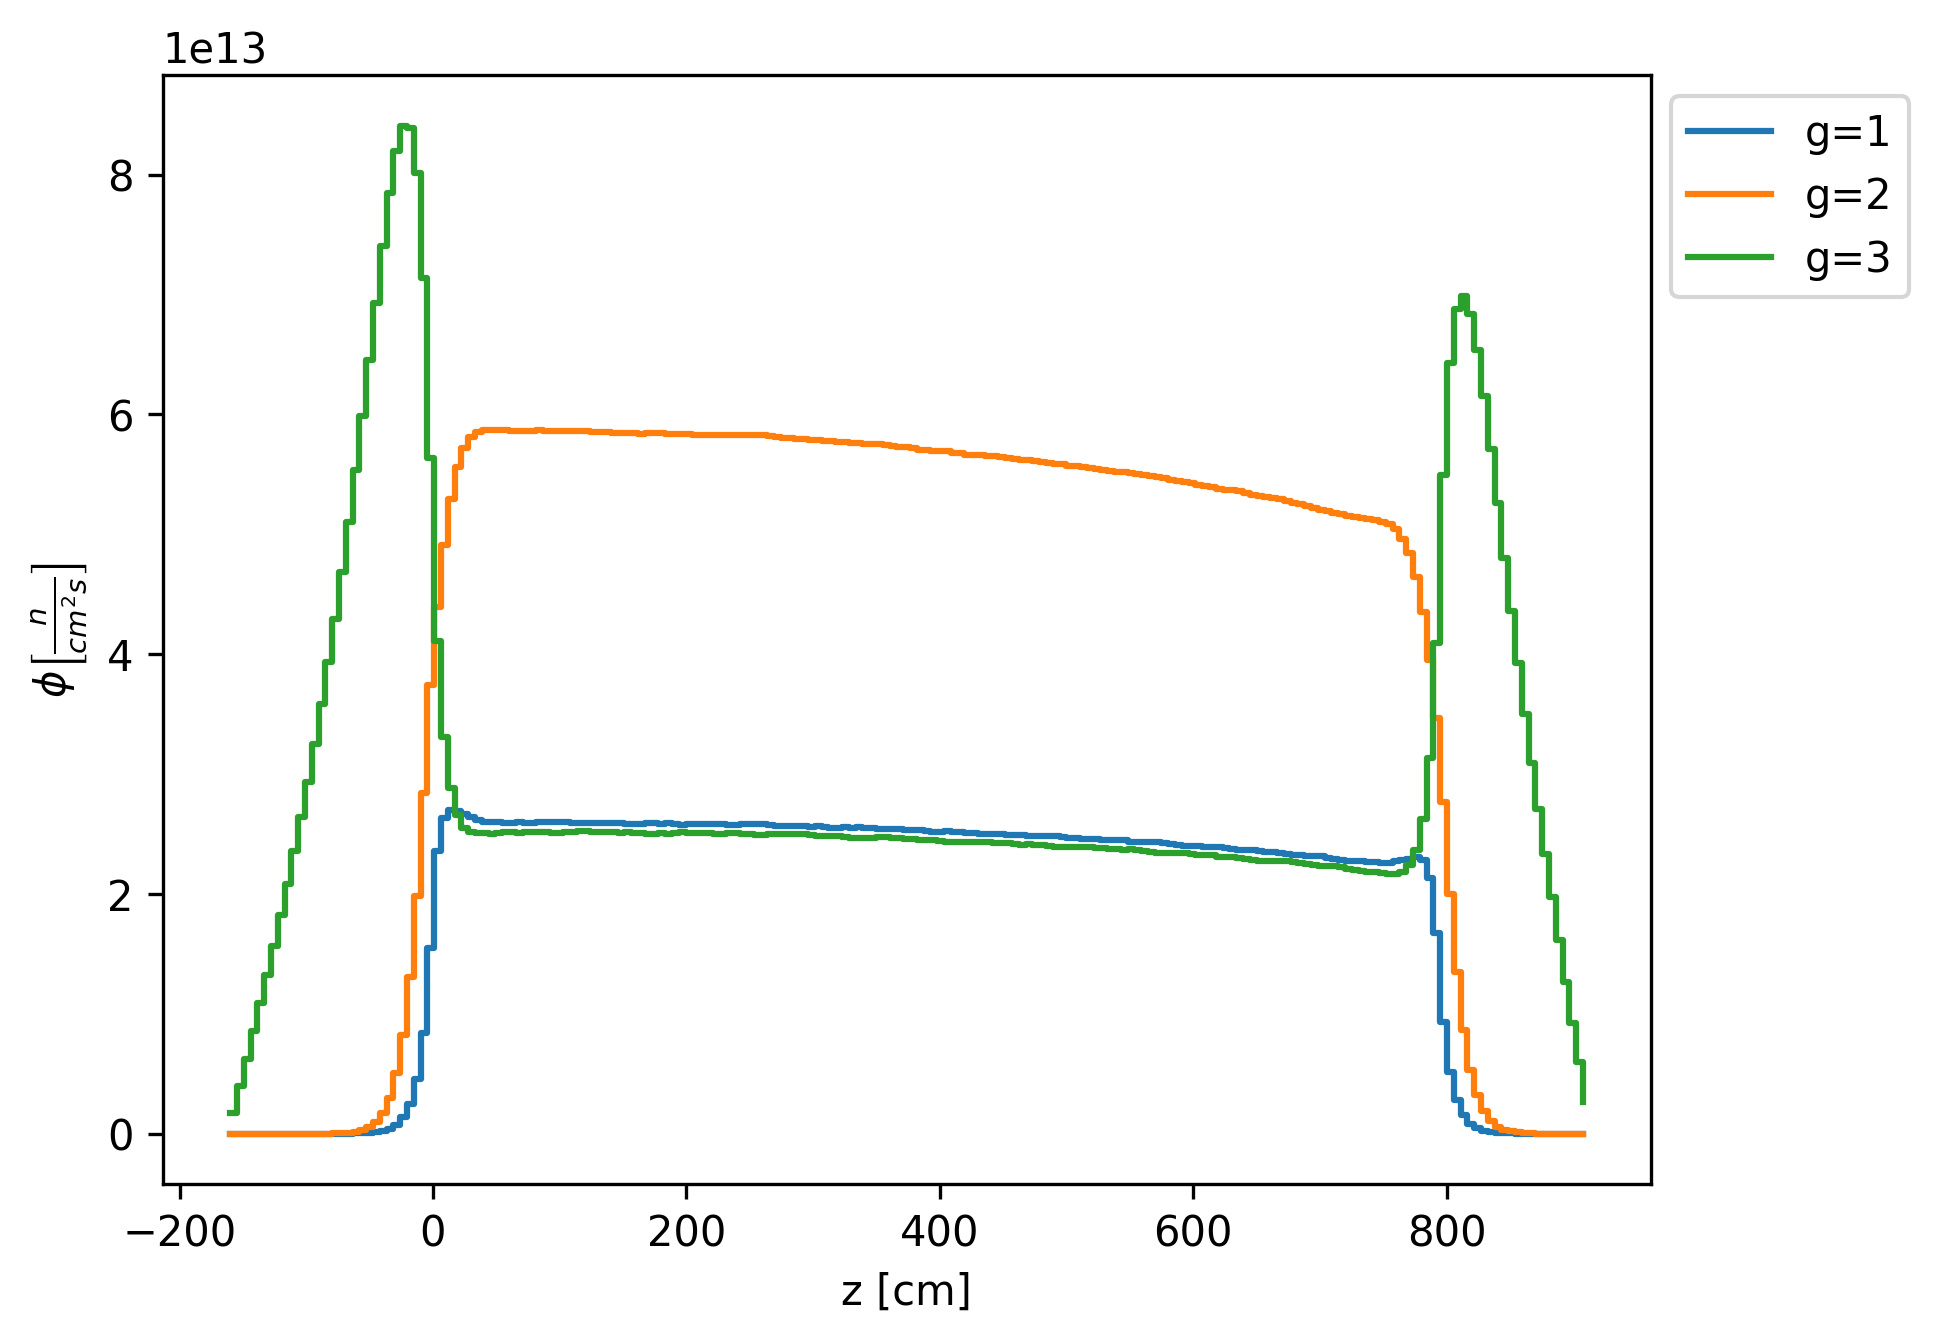
\includegraphics[width=\linewidth]{figures/serpent26G-noLBP-1200-collapse}
		\caption{Serpent.}
	\end{subfigure}
	\hfill
	\caption{Axial neutron flux for 3 groups.}
	\label{fig:assembly-noLBP-1200-flux}
\end{figure}

\begin{figure}[htbp!]
	\centering
	\begin{subfigure}[t]{0.4\textwidth}
		\centering
		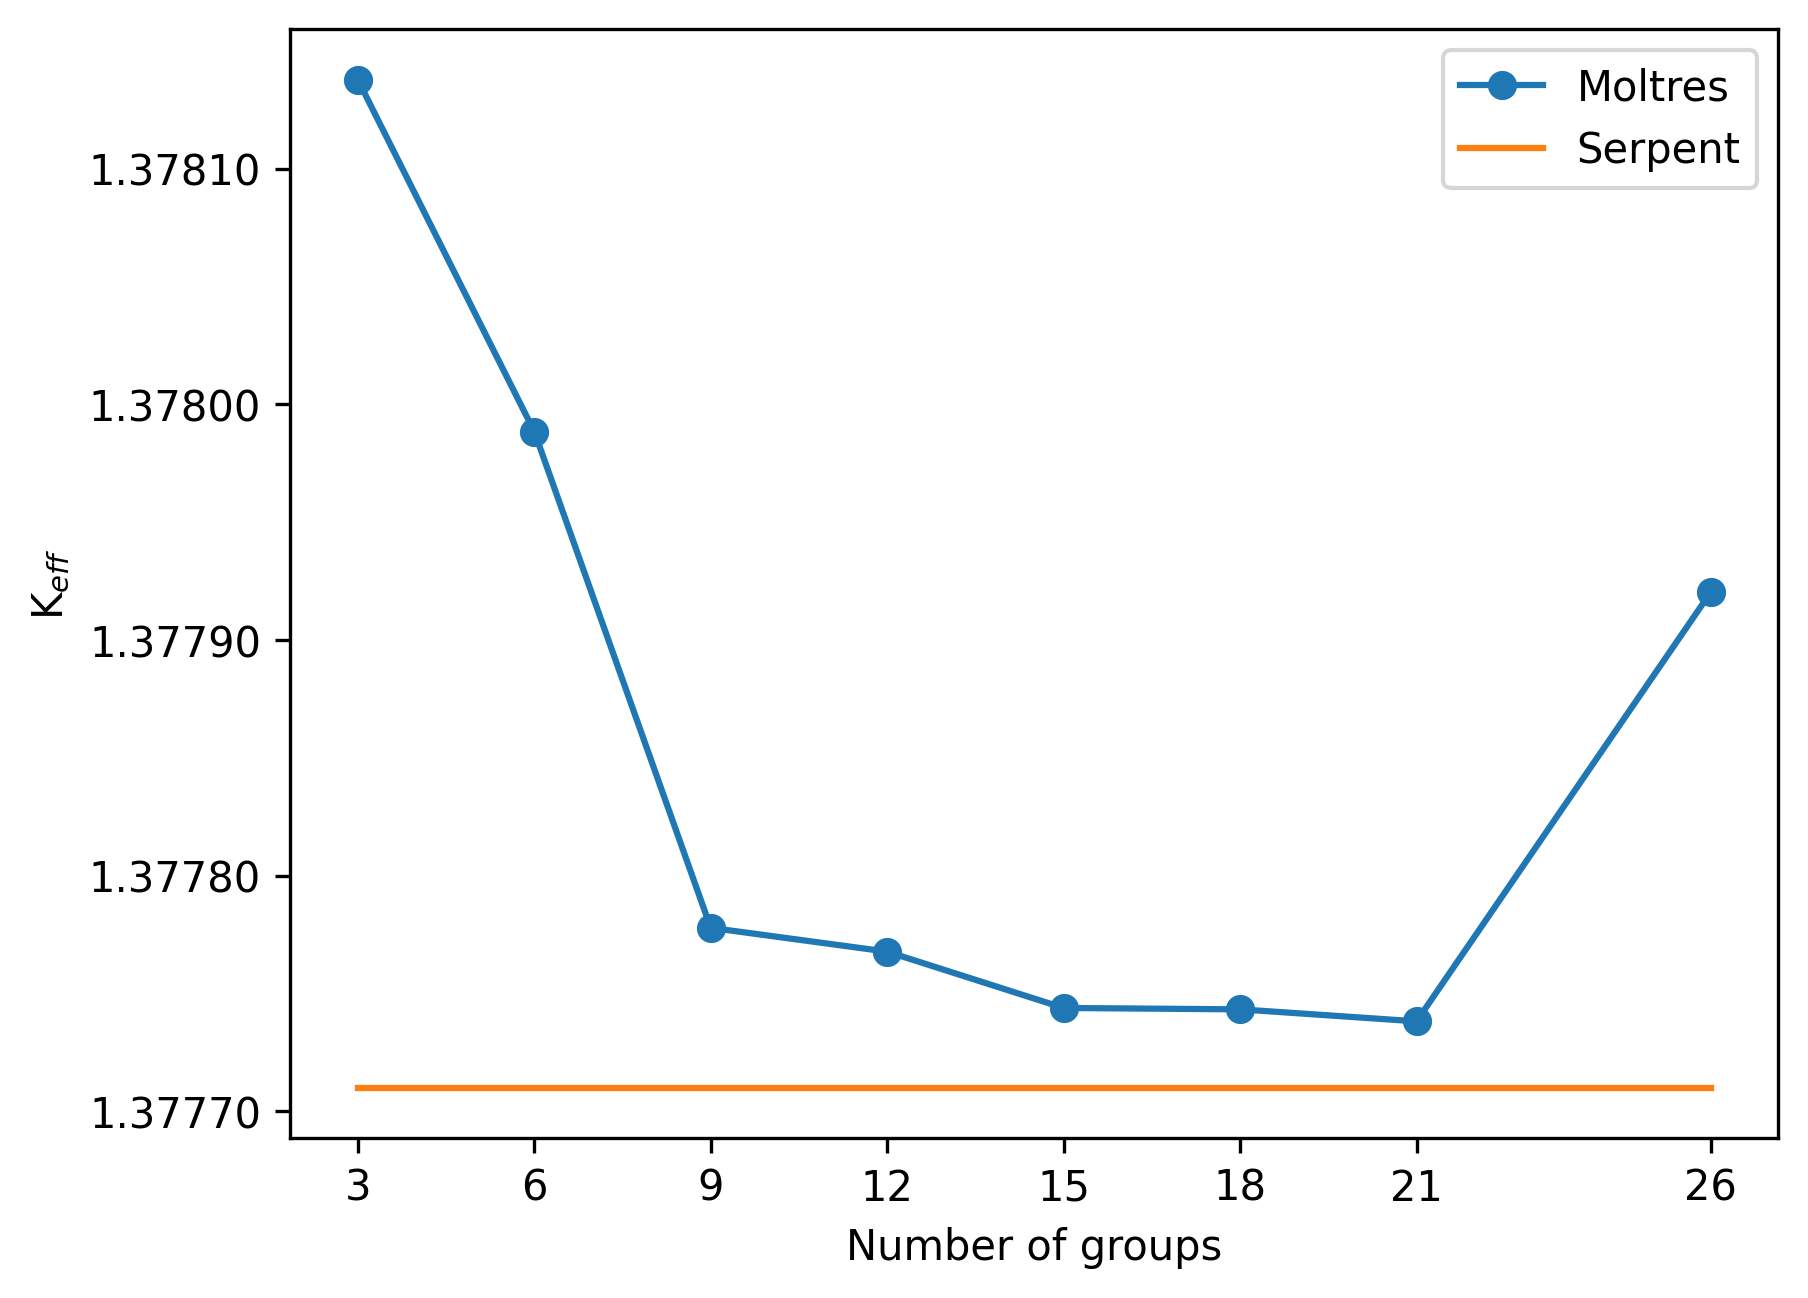
\includegraphics[width=\linewidth]{figures/keff-noLBP-1200}
		\caption{Multiplication factor.}
	\end{subfigure}
	\begin{subfigure}[t]{0.4\textwidth}
		\centering
		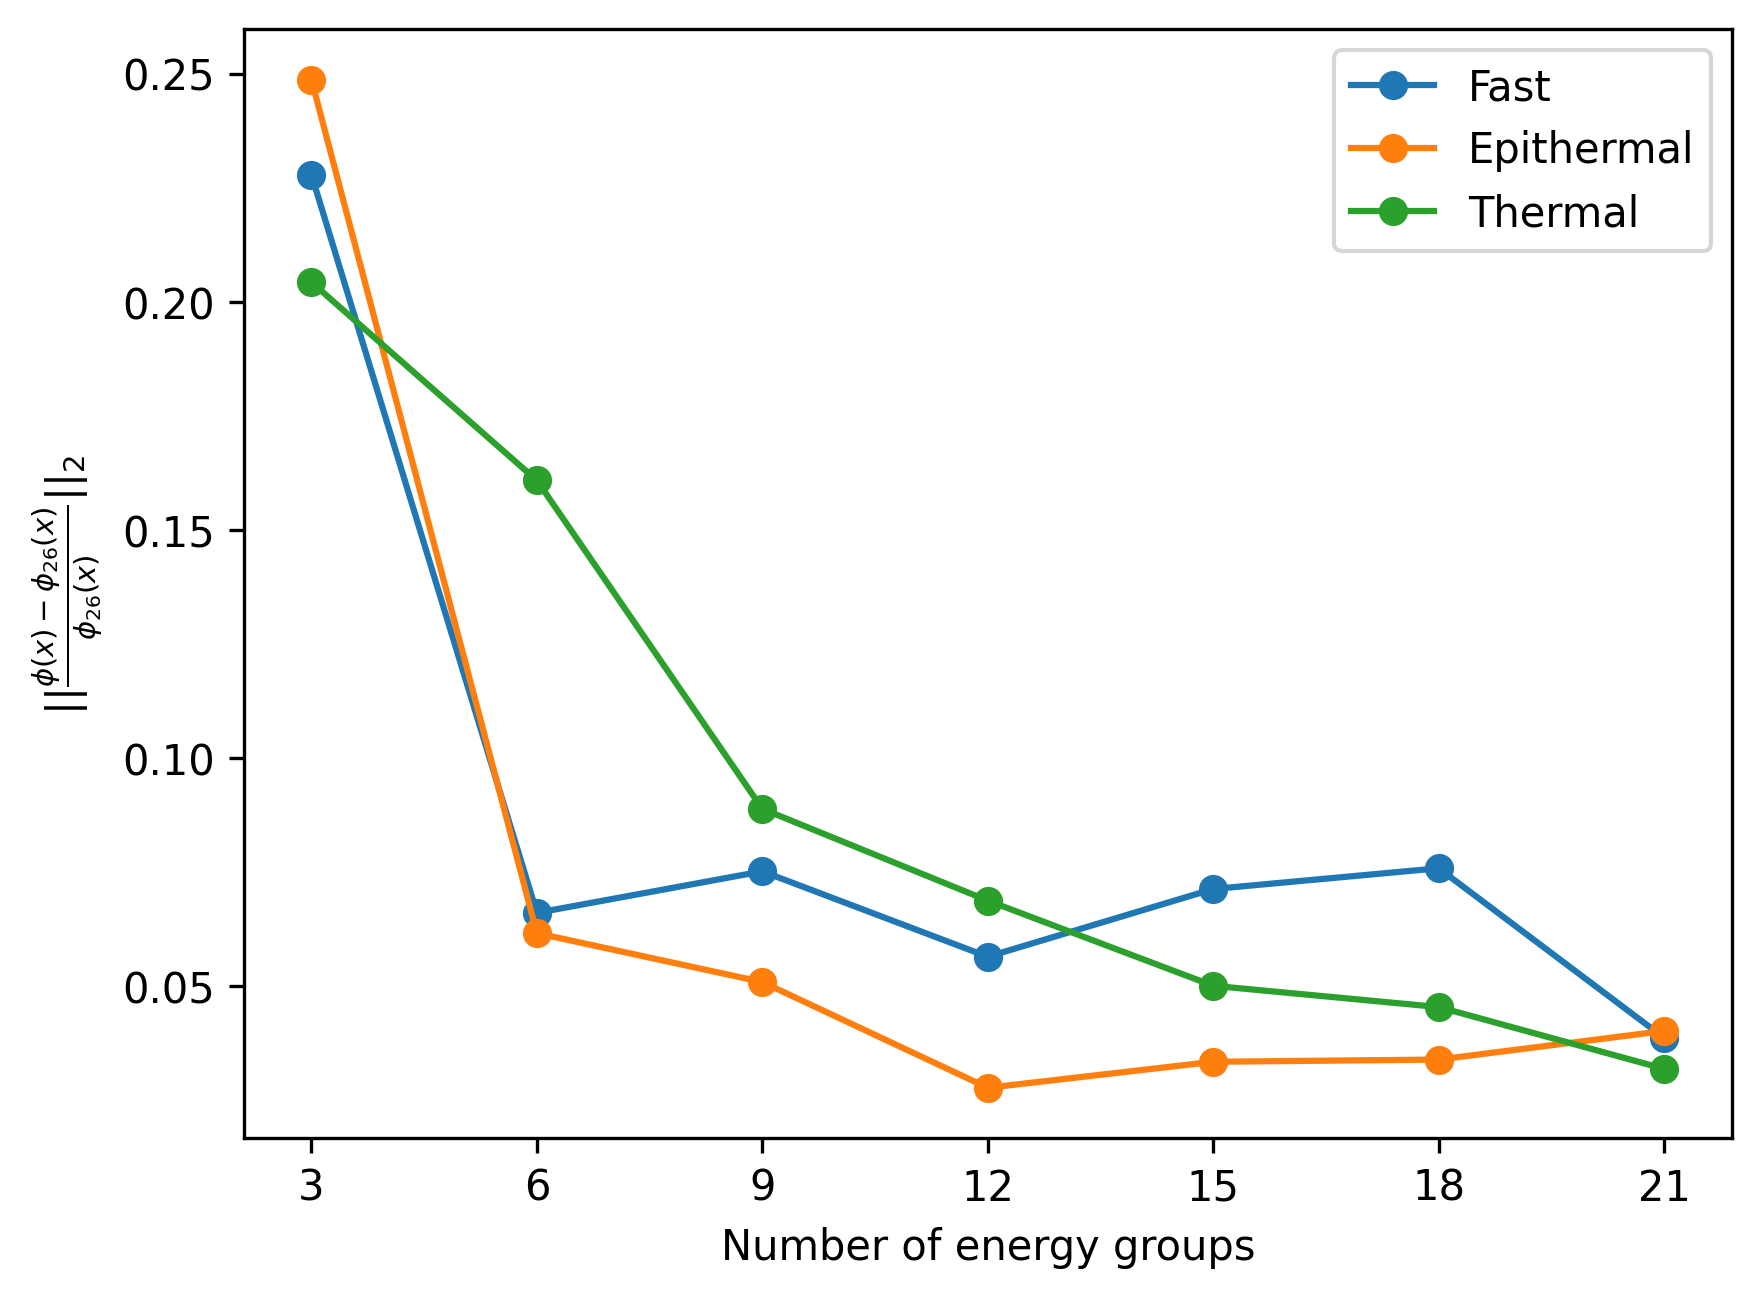
\includegraphics[width=\linewidth]{figures/noLBP-1200-er-final}
		\caption{L$_2$-norm relative error.}
	\end{subfigure}
	\hfill
	\caption{Effect of different number of energy group structures over different parameters.}
	\label{fig:assembly-noLBP-1200}
\end{figure}

% LBP 600 
\begin{figure}[htbp!]
	\centering
	\begin{subfigure}[t]{0.4\textwidth}
		\centering
		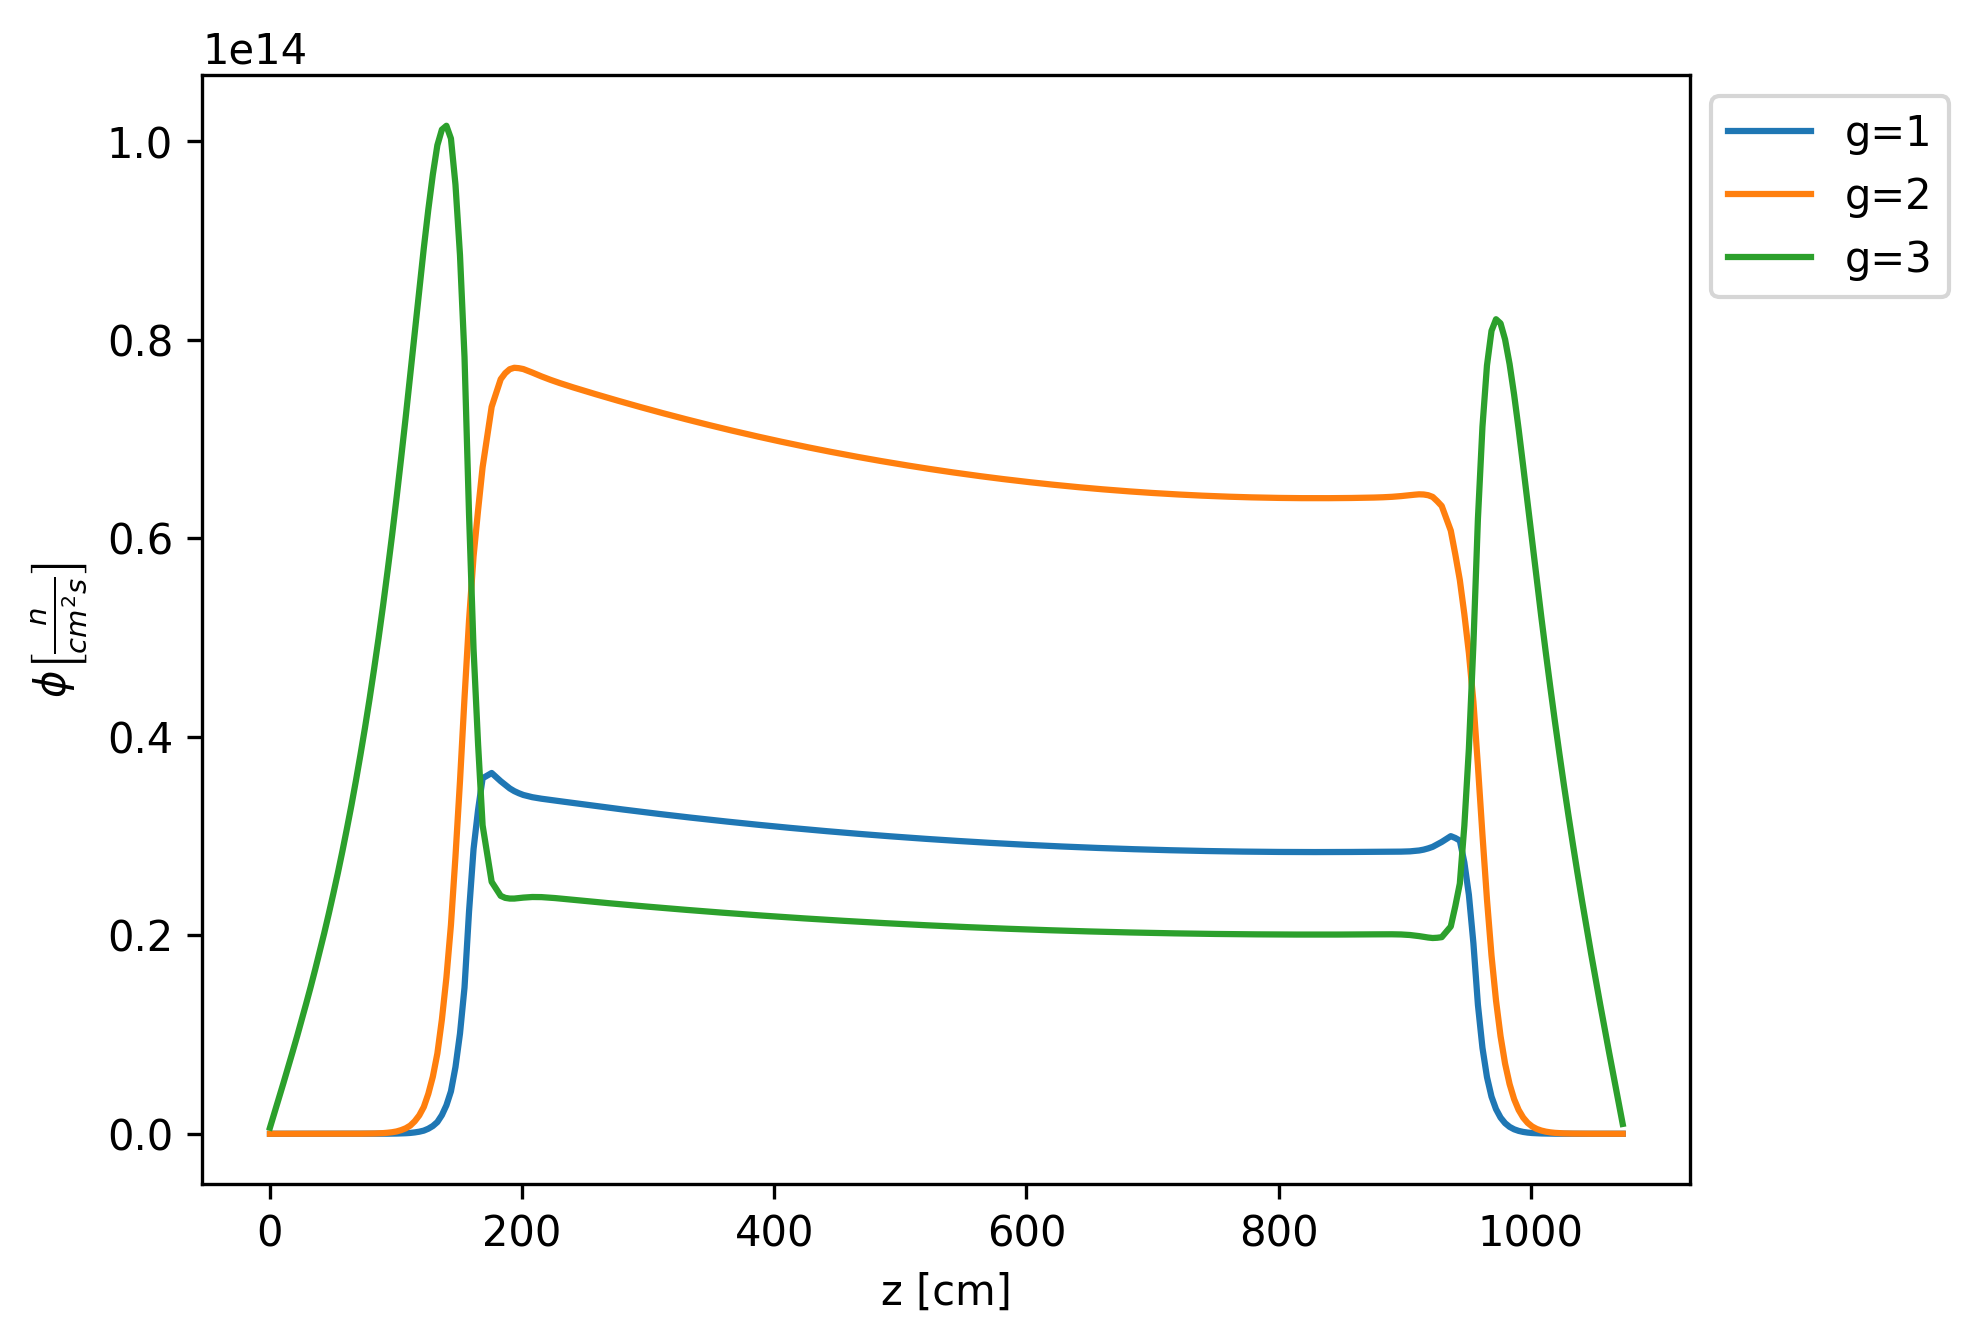
\includegraphics[width=\linewidth]{figures/3D-assembly-LBP-600-26G}
		\caption{Moltres.}
	\end{subfigure}
	\begin{subfigure}[t]{0.4\textwidth}
		\centering
		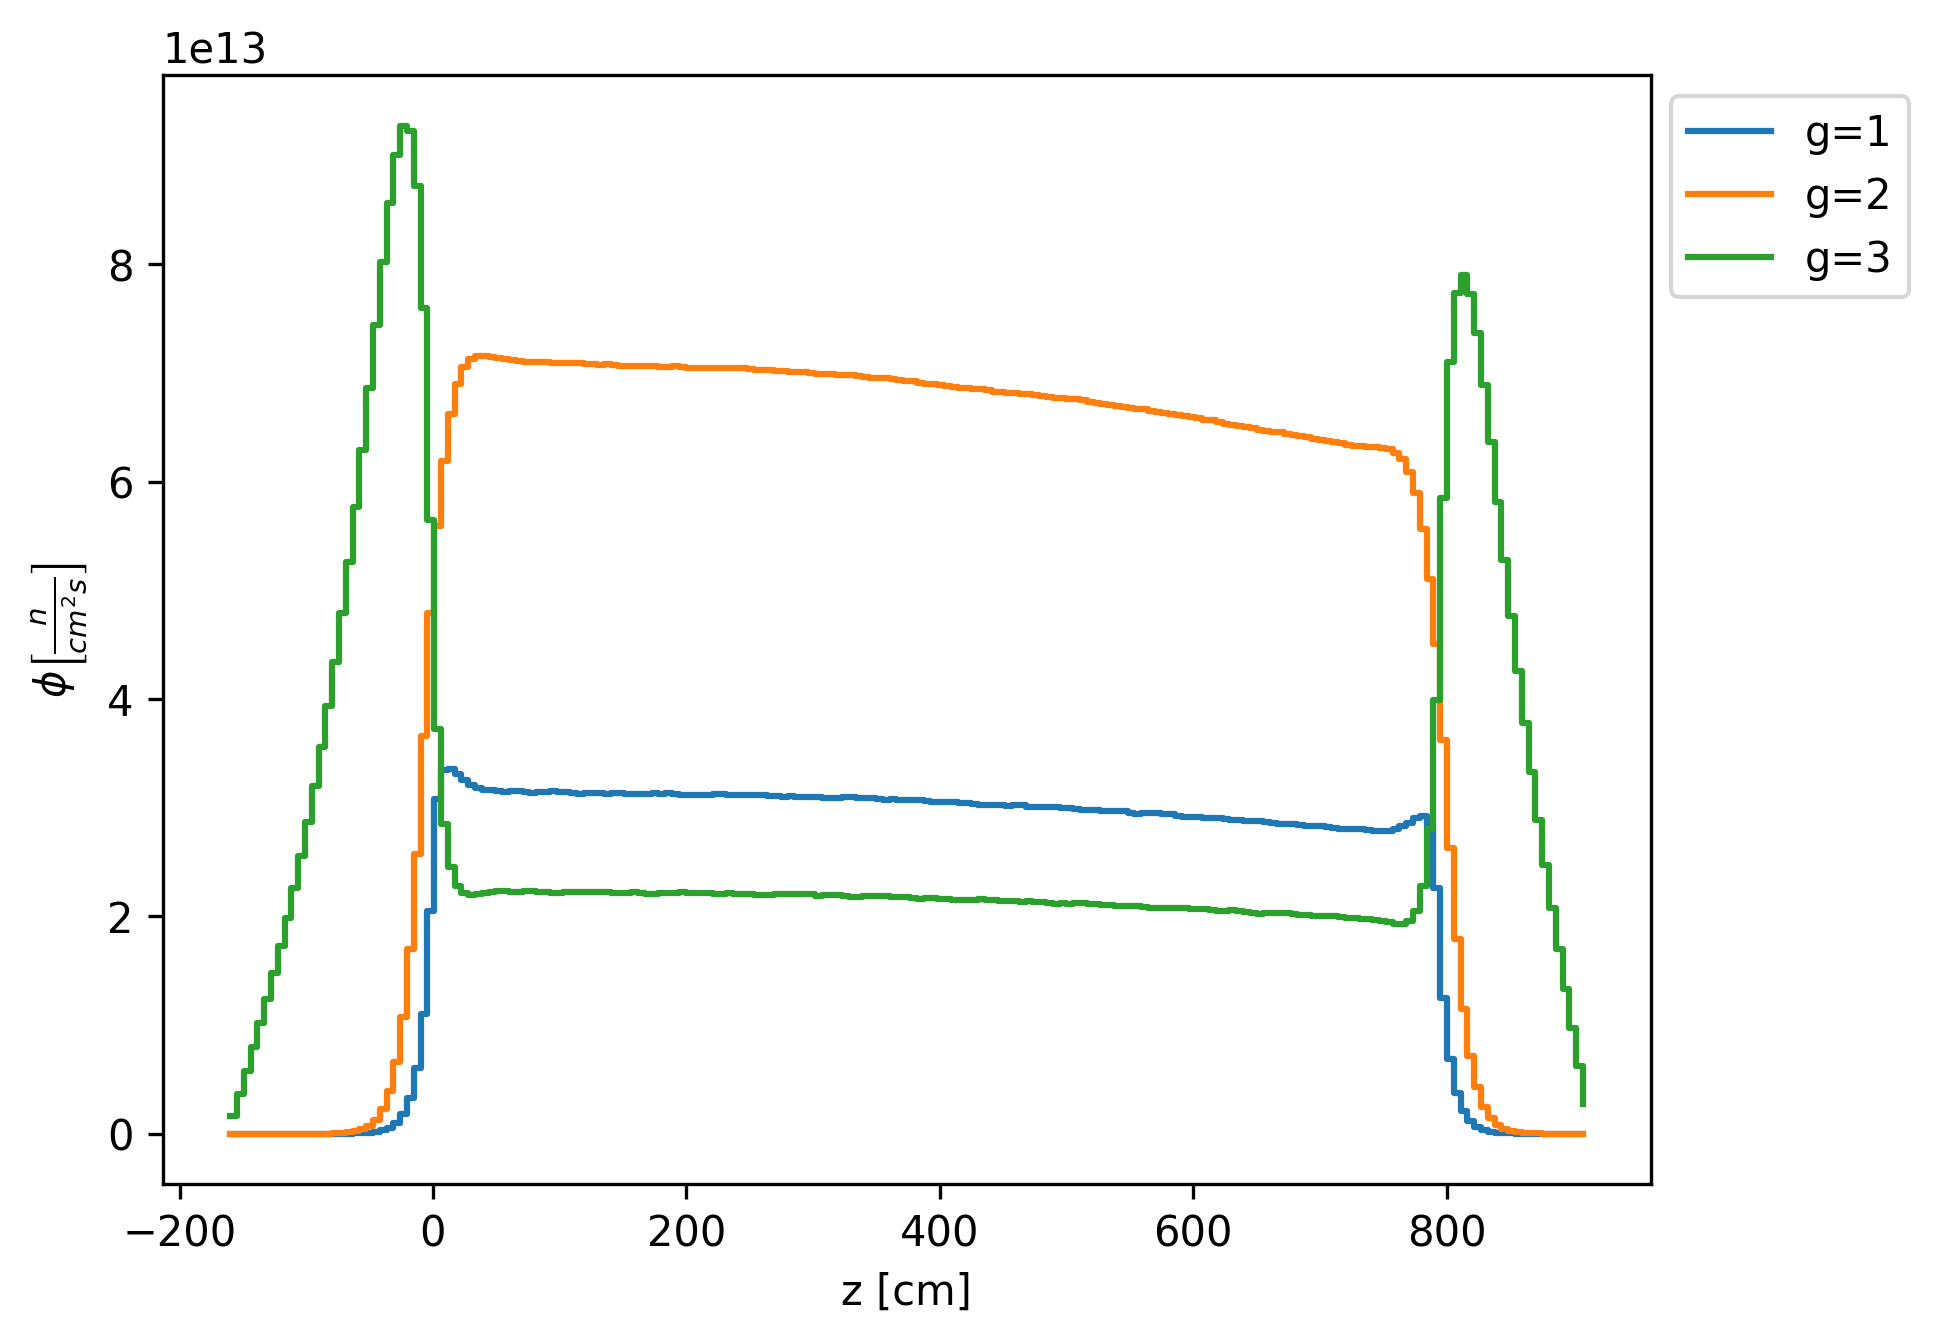
\includegraphics[width=\linewidth]{figures/serpent26G-LBP-600-collapse}
		\caption{Serpent.}
	\end{subfigure}
	\hfill
	\caption{Axial neutron flux for 3 groups.}
	\label{fig:assembly-LBP-600-flux}
\end{figure}

\begin{figure}[htbp!]
	\centering
	\begin{subfigure}[t]{0.4\textwidth}
		\centering
		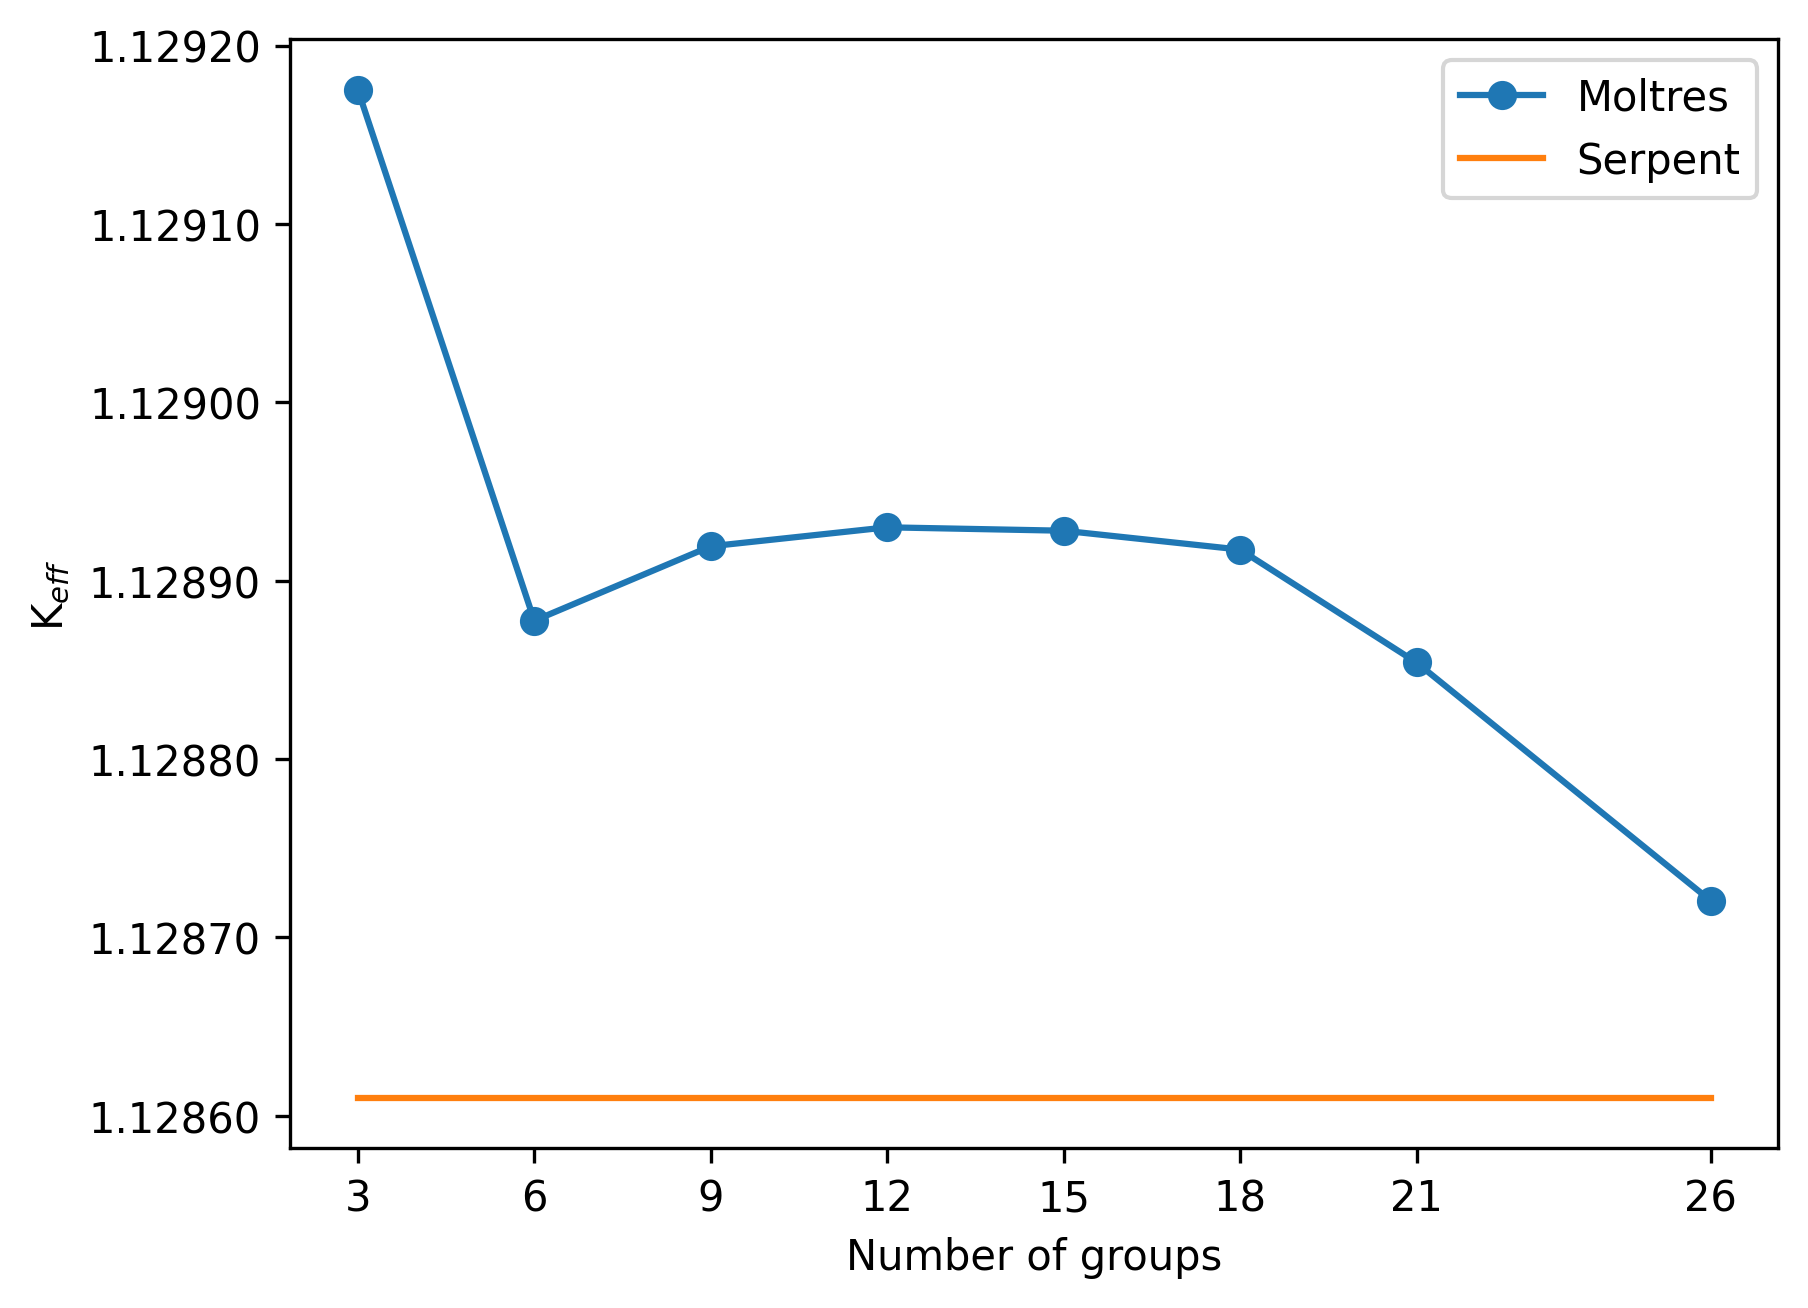
\includegraphics[width=\linewidth]{figures/keff-LBP-600}
		\caption{Multiplication factor.}
	\end{subfigure}
	\begin{subfigure}[t]{0.4\textwidth}
		\centering
		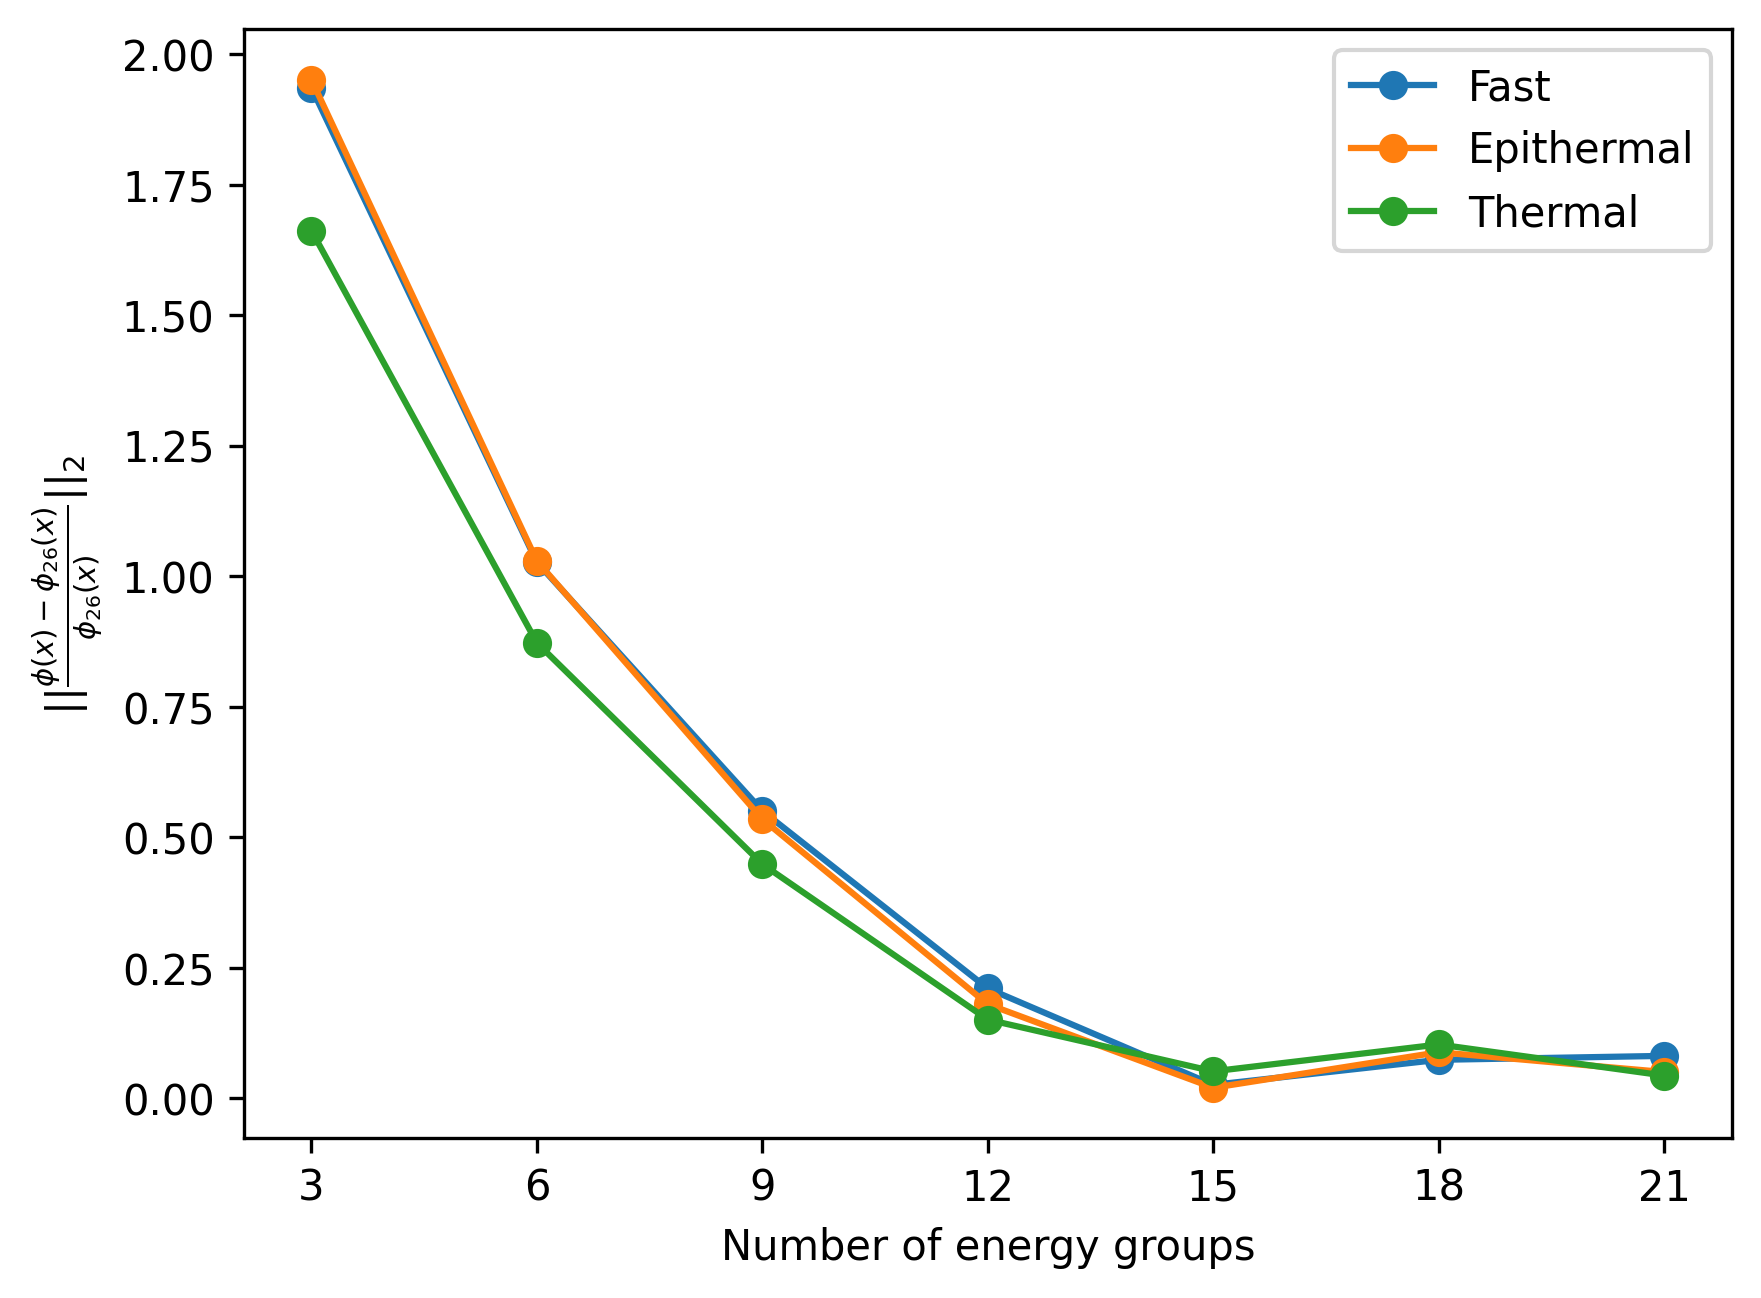
\includegraphics[width=\linewidth]{figures/LBP-600-er-final}
		\caption{L$_2$-norm relative error.}
	\end{subfigure}
	\hfill
	\caption{Effect of different number of energy group structures over different parameters.}
	\label{fig:assembly-LBP-600}
\end{figure}

\begin{figure}[htbp!]
	\centering
	\begin{subfigure}[t]{0.4\textwidth}
		\centering
		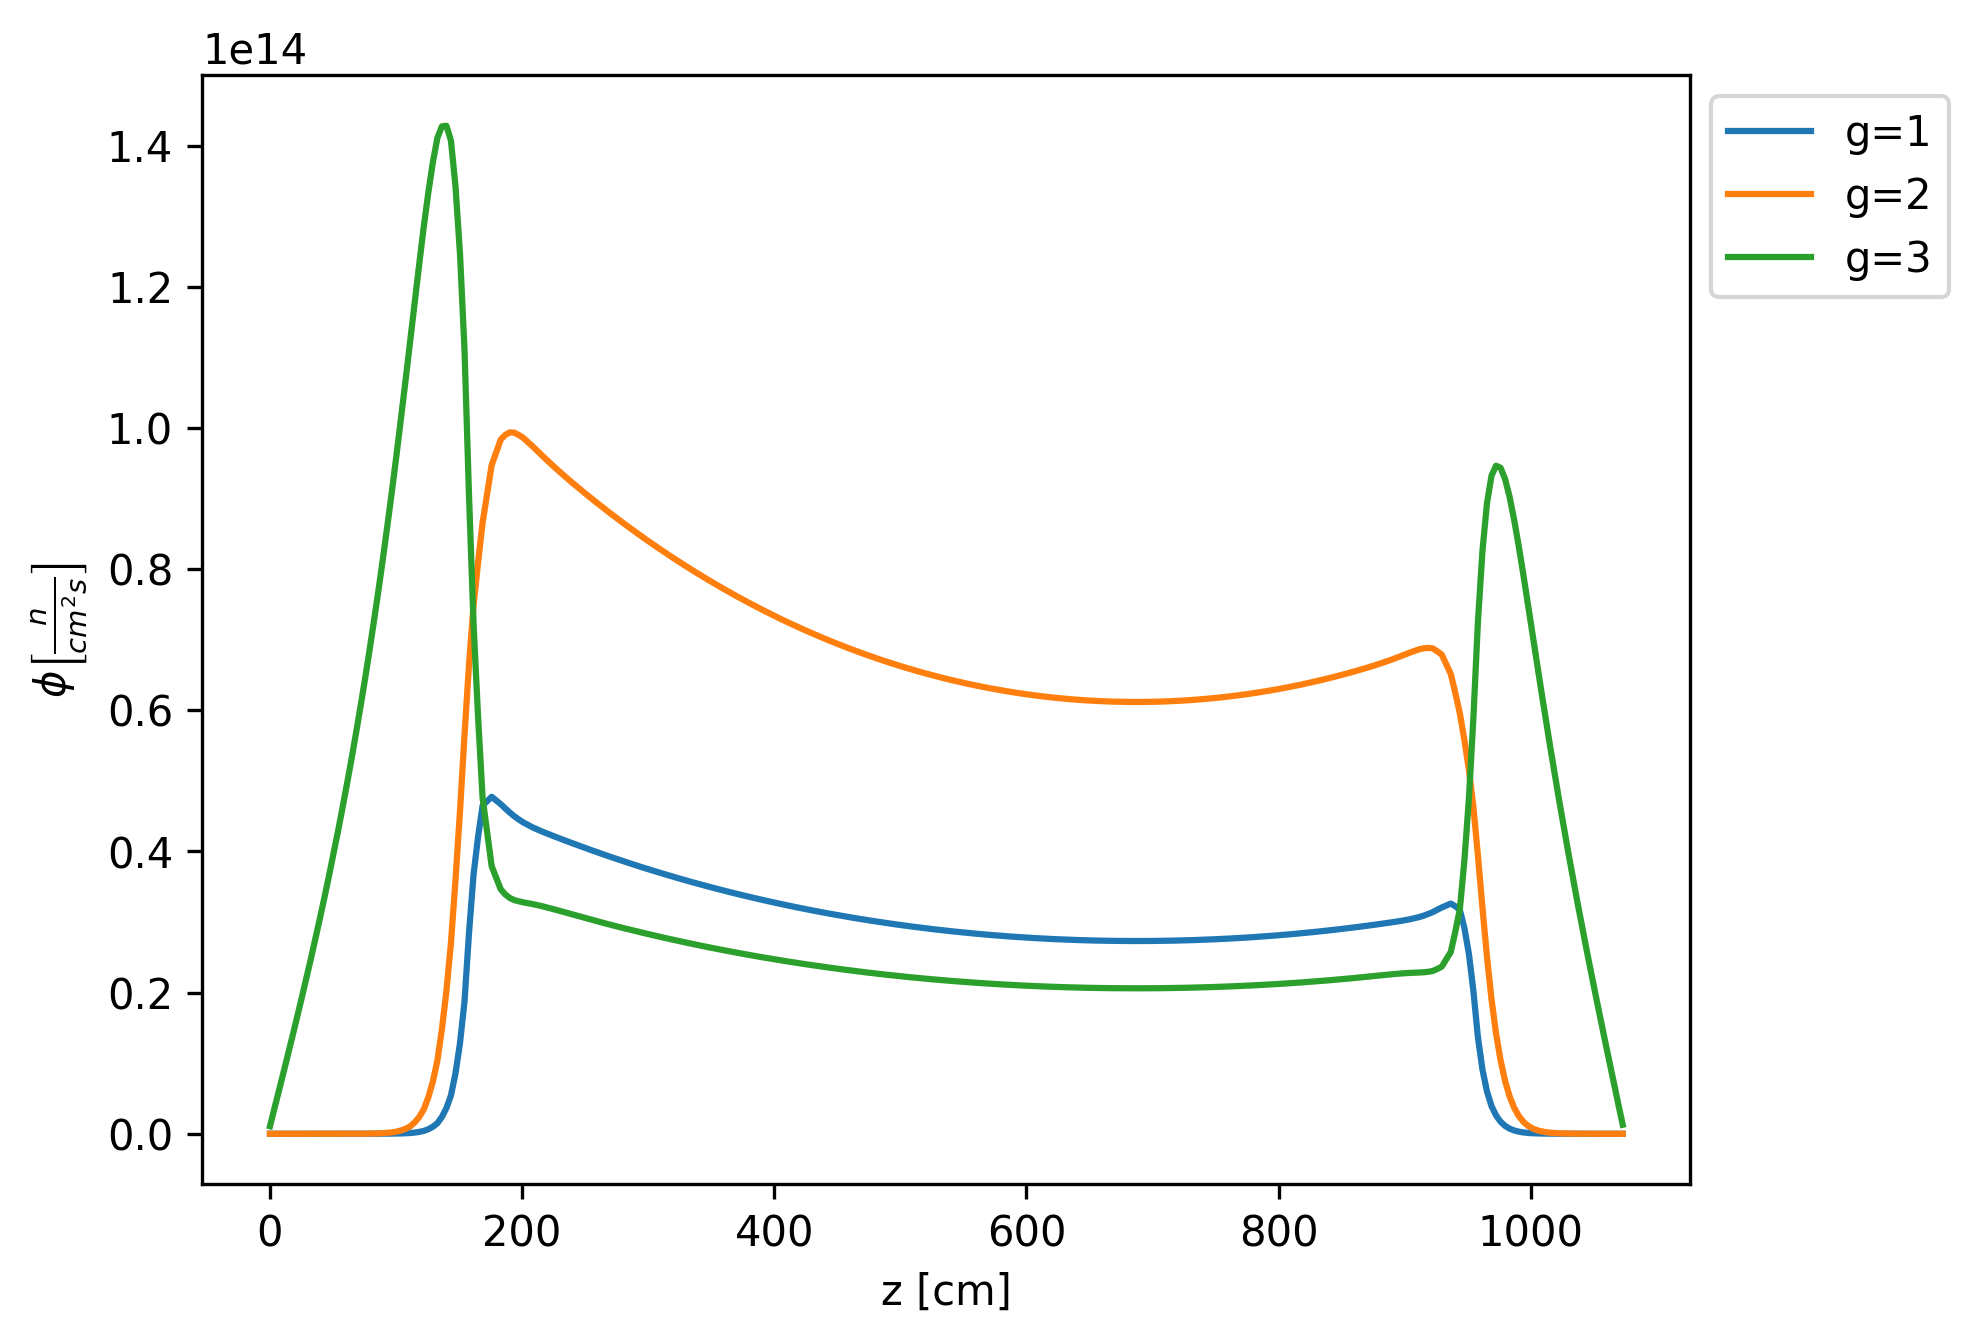
\includegraphics[width=\linewidth]{figures/3D-assembly-LBP-1200-26G}
		\caption{Moltres.}
	\end{subfigure}
	\begin{subfigure}[t]{0.4\textwidth}
		\centering
		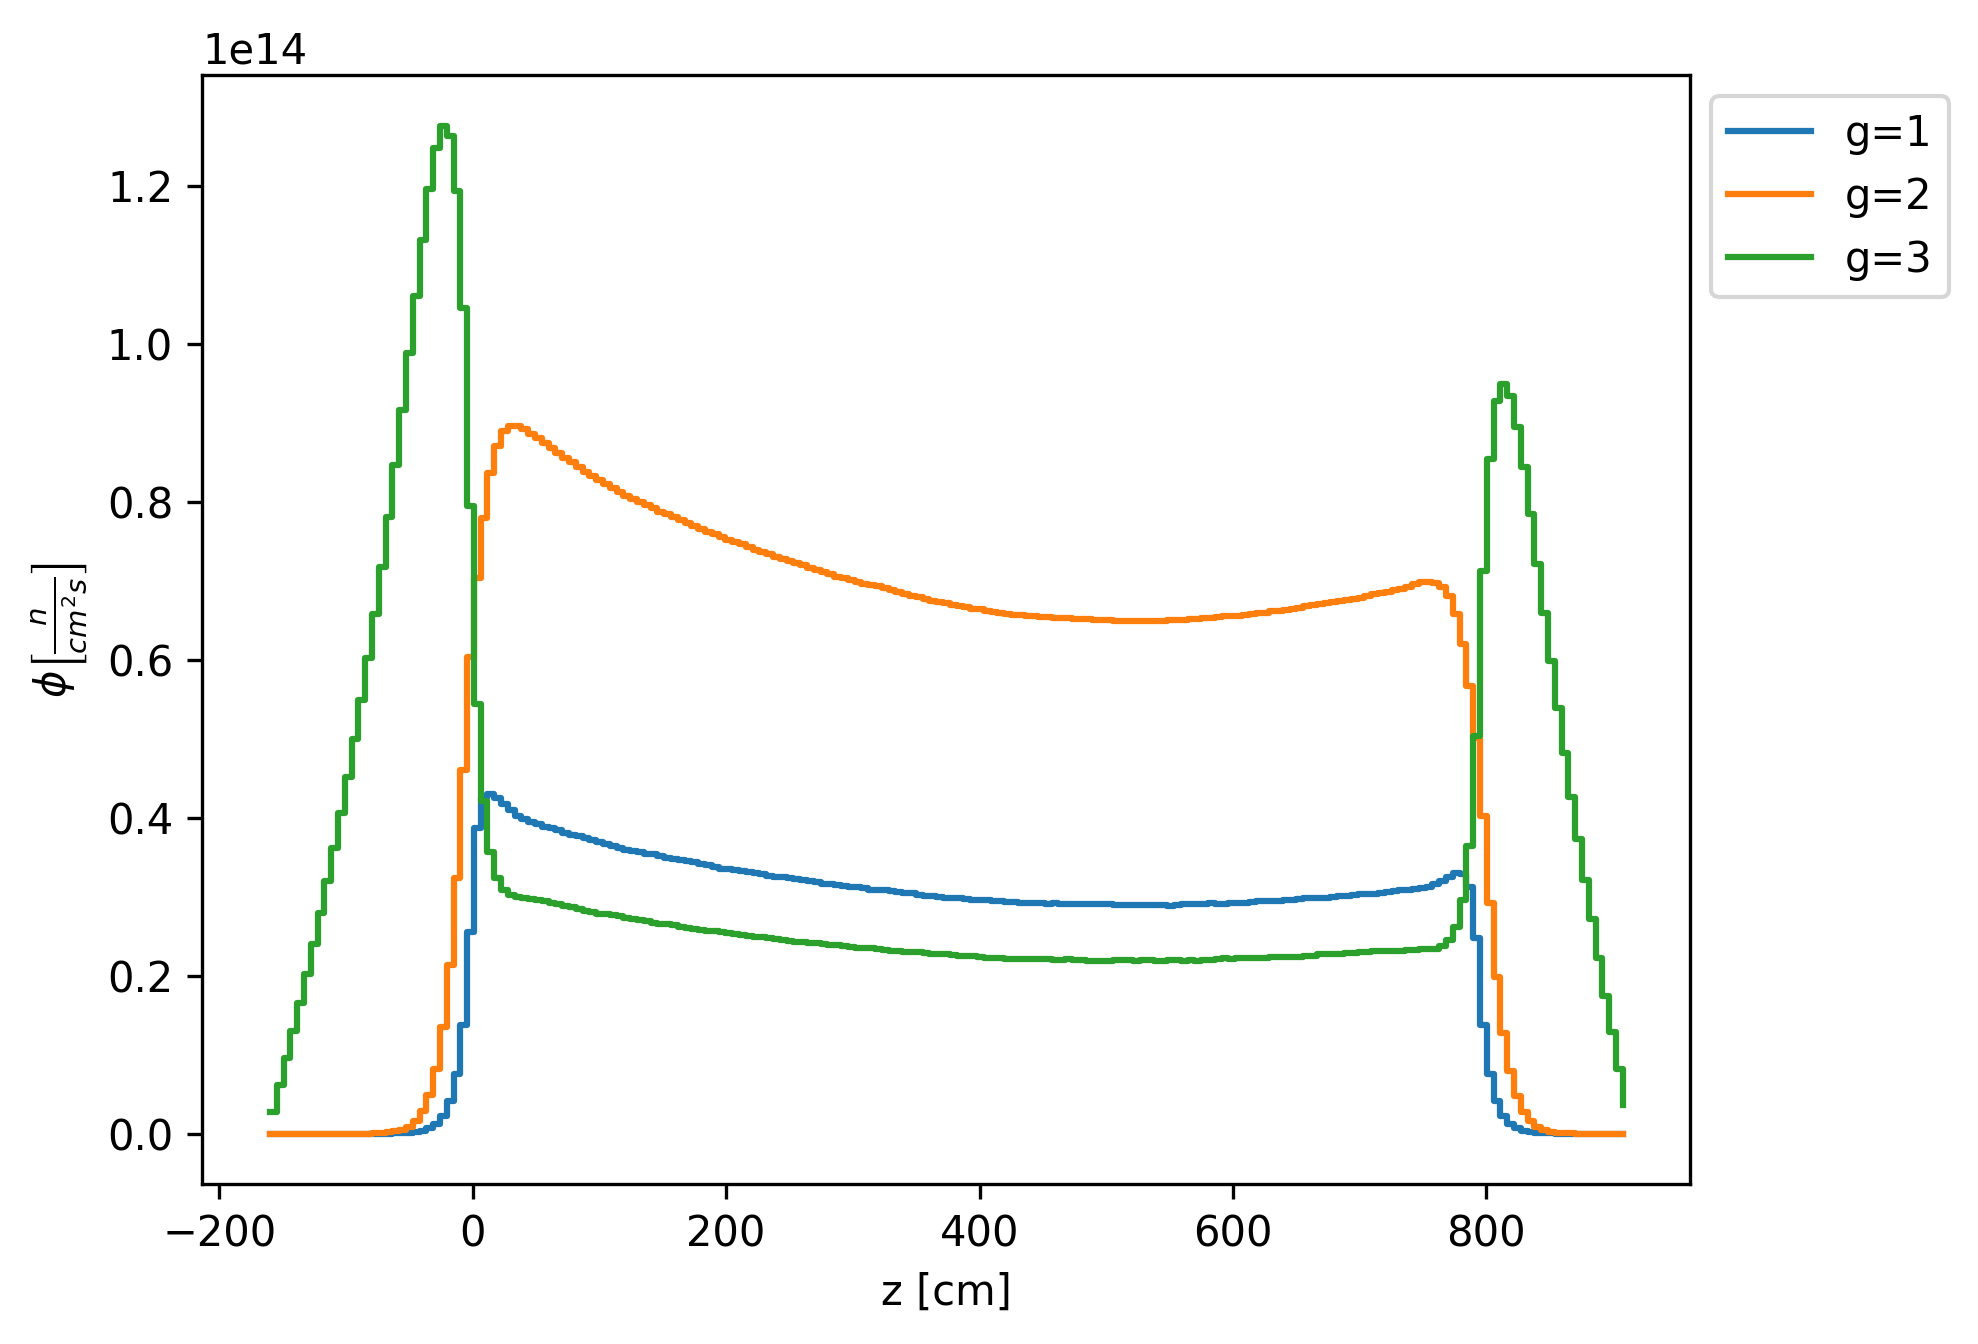
\includegraphics[width=\linewidth]{figures/serpent26G-LBP-1200-collapse}
		\caption{Serpent.}
	\end{subfigure}
	\hfill
	\caption{Axial neutron flux for 3 groups.}
	\label{fig:assembly-LBP-1200-flux}
\end{figure}

% LBP 1200 
\begin{figure}[htbp!]
	\centering
	\begin{subfigure}[t]{0.4\textwidth}
		\centering
		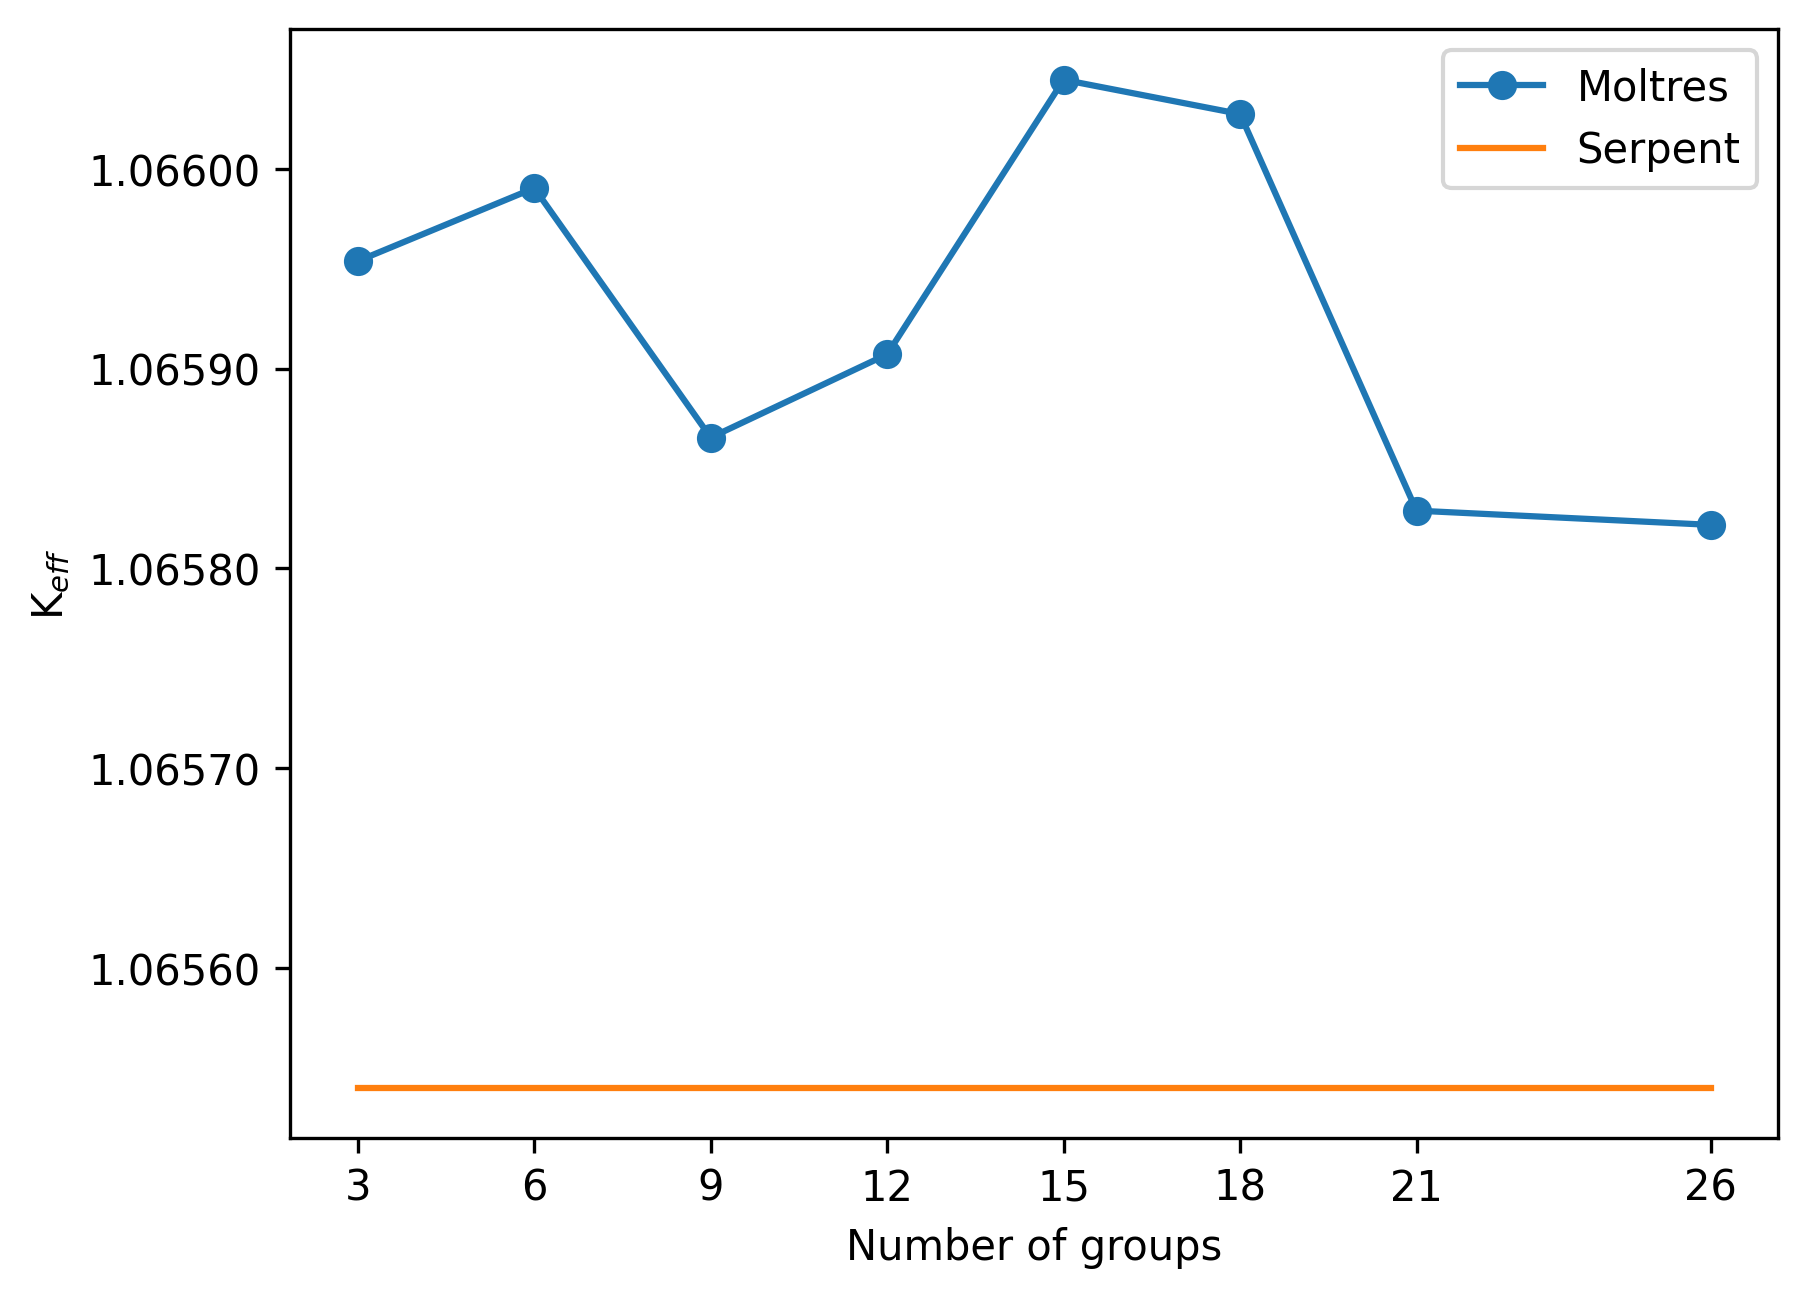
\includegraphics[width=\linewidth]{figures/keff-LBP-1200}
		\caption{Multiplication factor.}
	\end{subfigure}
	\begin{subfigure}[t]{0.4\textwidth}
		\centering
		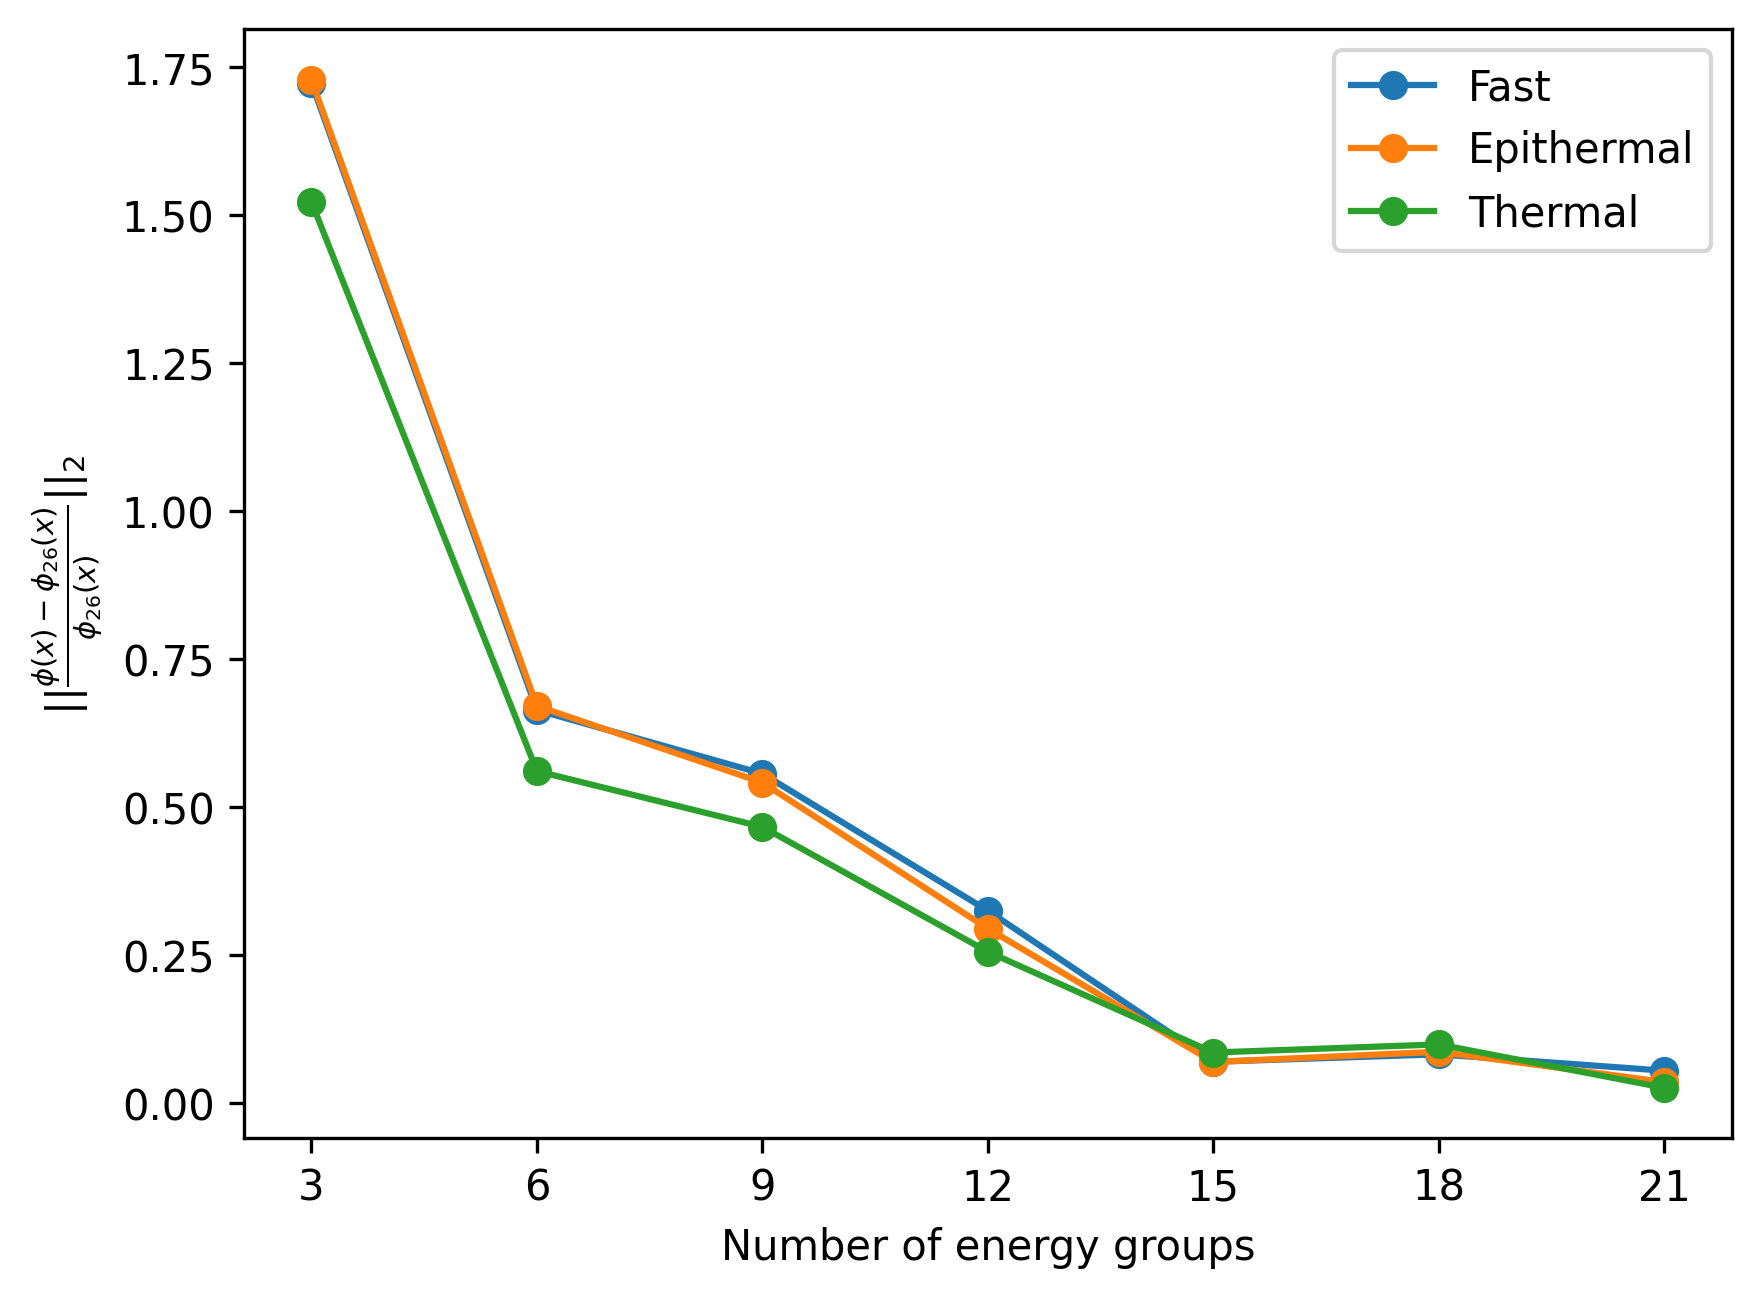
\includegraphics[width=\linewidth]{figures/LBP-1200-er-final}
		\caption{L$_2$-norm relative error.}
	\end{subfigure}
	\hfill
	\caption{Effect of different number of energy group structures over different parameters.}
	\label{fig:assembly-LBP-1200}
\end{figure}

% Time and memory
\begin{figure}[htbp!]
	\centering
	\begin{subfigure}[t]{0.4\textwidth}
		\centering
		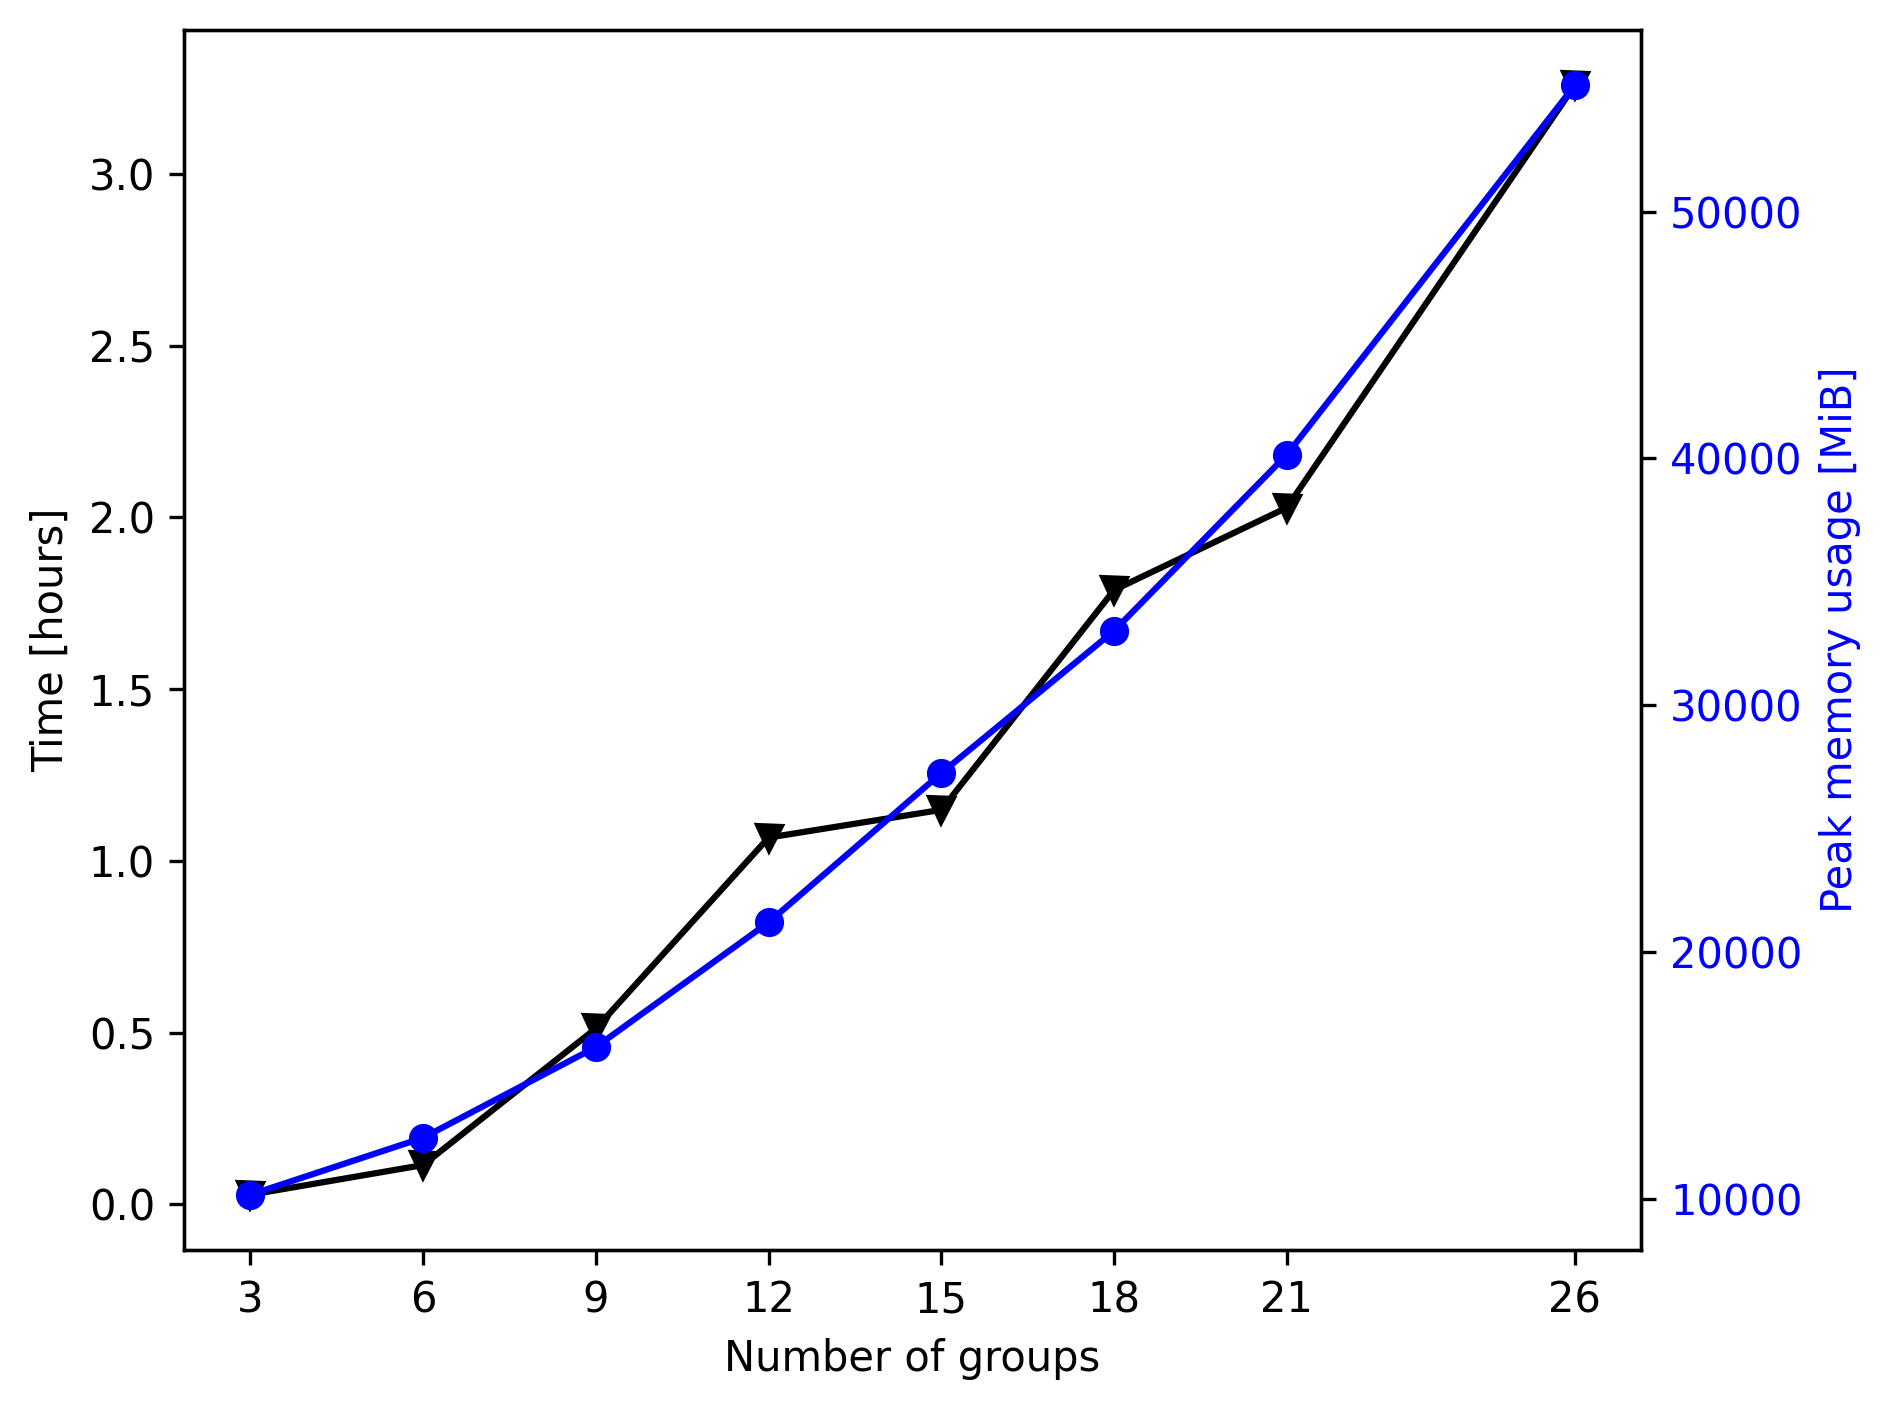
\includegraphics[width=\linewidth]{figures/time-noLBP-600}
		\caption{No LBP and 600 K.}
	\end{subfigure}
	\begin{subfigure}[t]{0.4\textwidth}
		\centering
		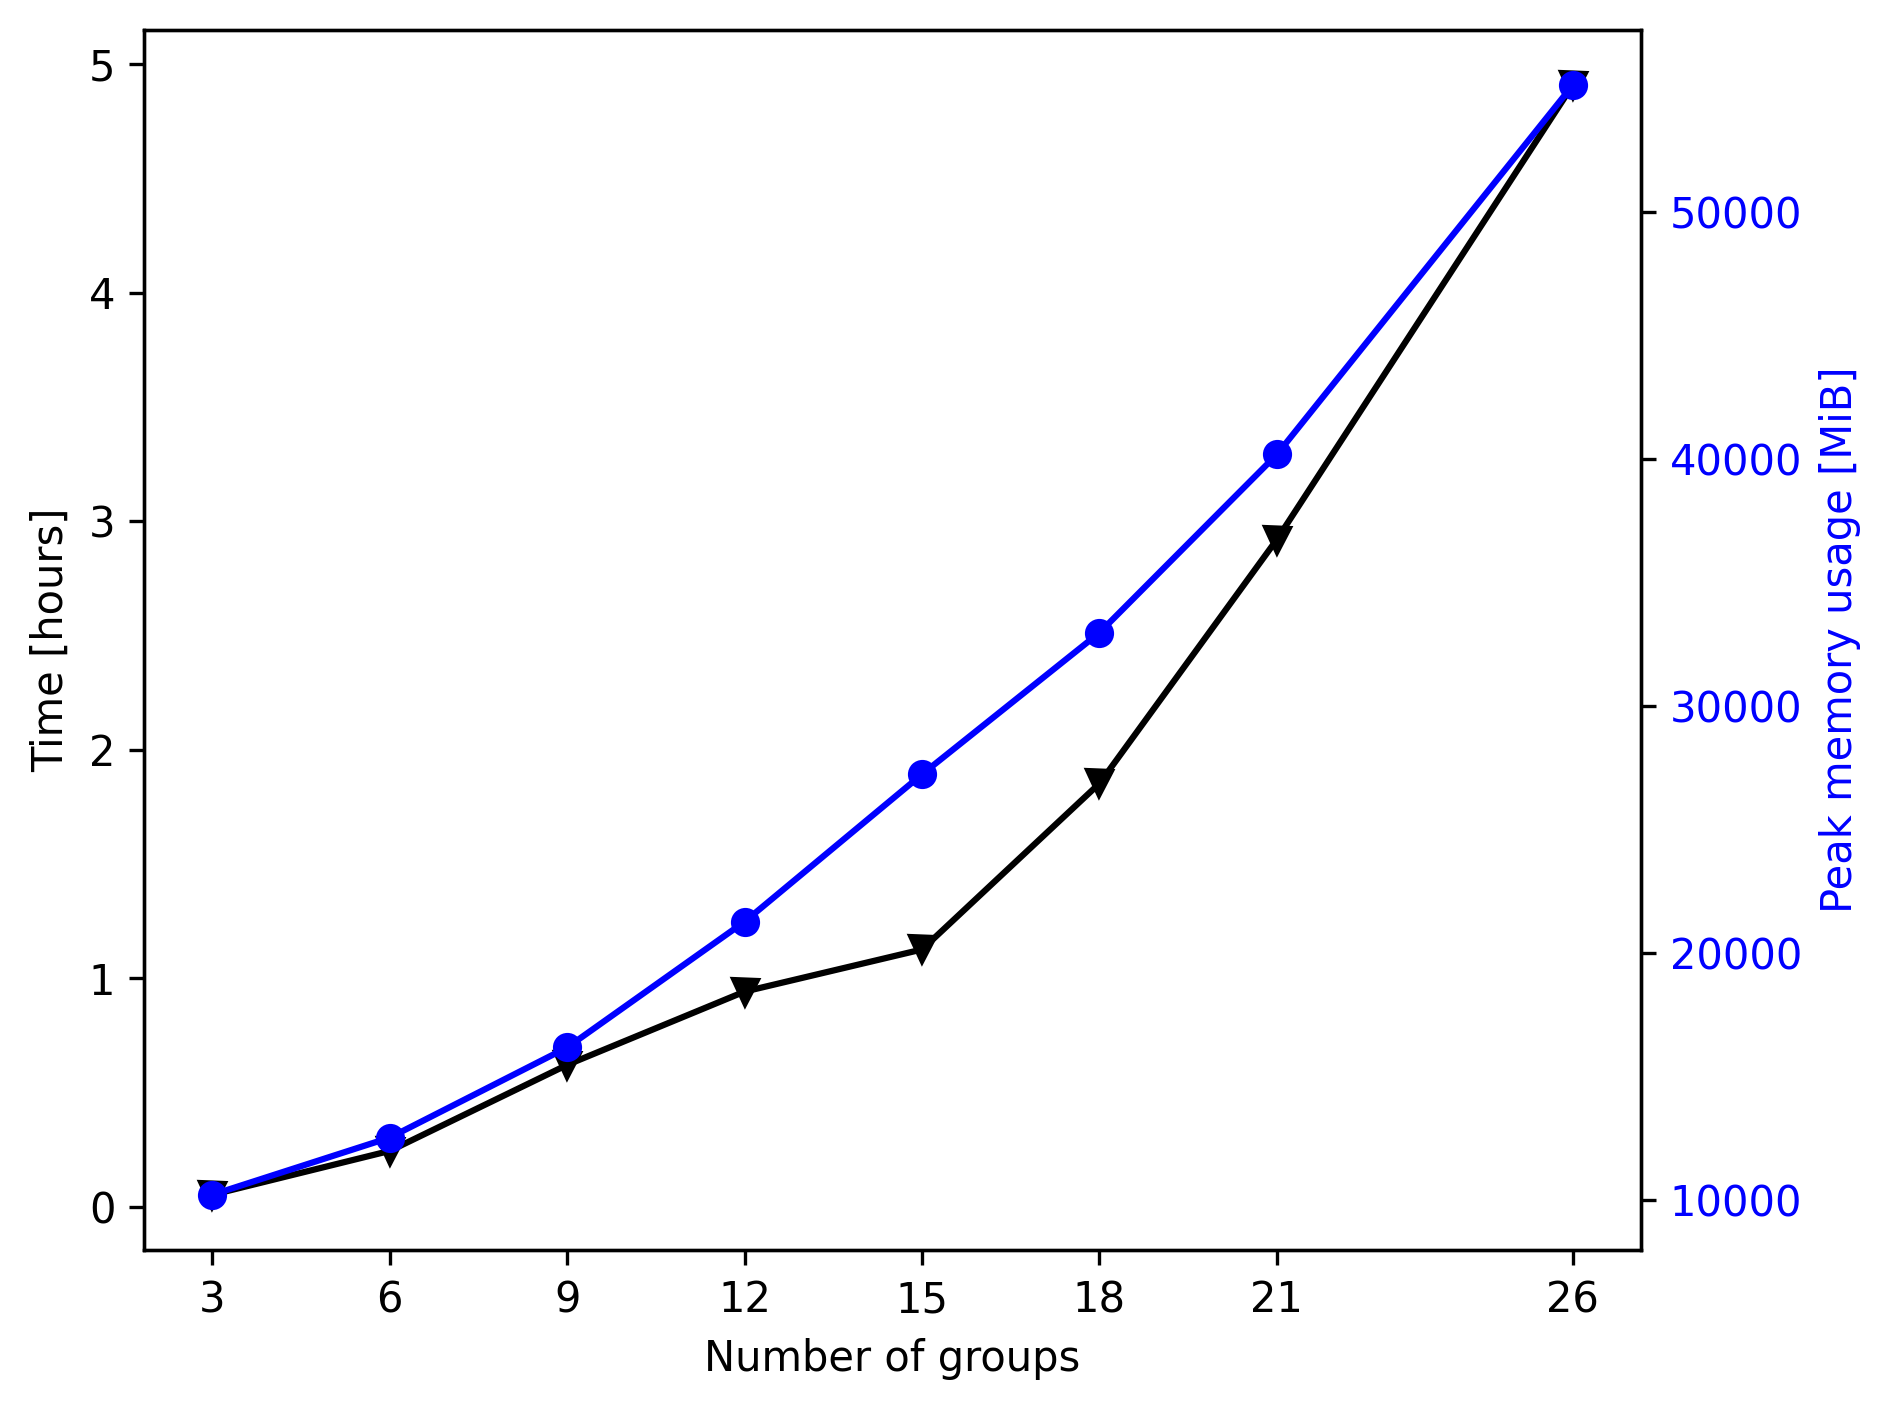
\includegraphics[width=\linewidth]{figures/time-LBP-1200}
		\caption{LBP and 1200 K.}
	\end{subfigure}
	\hfill
	\caption{Effect of different number of energy group structures over computational time and memory requirements.}
	\label{fig:assembly-time}
\end{figure}

\begin{table}[htbp!]
  \centering
  \caption{Parametric study on the energy group limits. Values expressed in percentage.}
  \begin{tabular}{@{}l|l|l| S[table-format=2.1] S[table-format=2.1] S[table-format=2.1] S[table-format=2.1] S[table-format=2.1] }
  \toprule
	LBP                  & Temperature {[}K{]}   & Flux       & \multicolumn{1}{c@{}}{15a} & \multicolumn{1}{c@{}}{15b}  & \multicolumn{1}{c@{}}{15c}  & \multicolumn{1}{c@{}}{15d}  & \multicolumn{1}{c@{}}{15e}  \\
	\midrule
	\multirow{6}{*}{No}  & \multirow{3}{*}{600}  & Fast       & 7.9  & 8.0  & 8.2  & 8.1  & 9.1  \\
	                     &                       & Epithermal & 6.6  & 6.5  & 8.6  & 8.2  & 9.2  \\
	                     &                       & Thermal    & 8.8  & 8.5  & 10.6 & 10.7 & 12.9 \\ \cline{2-8}
	                     & \multirow{3}{*}{1200} & Fast       & 7.1  & 7.7  & 5.7  & 5.1  & 4.5  \\
	                     &                       & Epithermal & 3.3  & 3.9  & 6.2  & 5.1  & 3.4  \\
	                     &                       & Thermal    & 5.0  & 4.7  & 8.5  & 8.2  & 8.4  \\ \hline
	\multirow{6}{*}{Yes} & \multirow{3}{*}{600}  & Fast       & 24.0 & 24.8 & 2.6  & 2.3  & 3.7  \\
	                     &                       & Epithermal & 21.0 & 21.7 & 2.0  & 1.6  & 2.7  \\
	                     &                       & Thermal    & 18.1 & 18.8 & 5.2  & 5.5  & 5.7  \\ \cline{2-8}
	                     & \multirow{3}{*}{1200} & Fast       & 36.2 & 37.3 & 6.9  & 6.6  & 25.9 \\
	                     &                       & Epithermal & 33.2 & 34.2 & 6.9  & 6.5  & 25.1 \\
	                     &                       & Thermal    & 29.6 & 30.6 & 8.5  & 8.3  & 20.3 \\
	\midrule
	\multicolumn{2}{l}{Average}                  &            & 17.3 & 17.8 & 6.3  & 6.0  & 10.8 \\
	\bottomrule
  \end{tabular}
  \label{tab:accuracy15}
\end{table}


\section{Fullcore}

Dof/group = 160035
total dof = 2400525

Serpent: 
keff (600K) = 1.10869
keff (1200K) = 1.06138

Moltres:
keff (600K) = 1.1115000683
keff (1200K) = 1.0646803289


Figure \ref{fig:fullcoremodel}

Figure \ref{fig:fullcore-600-power}
Figure \ref{fig:fullcore-1200-power}

Figure \ref{fig:fullcore-detectors}

Figure \ref{fig:fullcore-600-axial1}
Figure \ref{fig:fullcore-600-axial2}
Figure \ref{fig:fullcore-600-radial1}

Figure \ref{fig:fullcore-1200-axial1}
Figure \ref{fig:fullcore-1200-axial2}
Figure \ref{fig:fullcore-1200-radial1}

\begin{figure}[htbp!]
	\centering
	\begin{subfigure}[t]{0.4\textwidth}
		\centering
		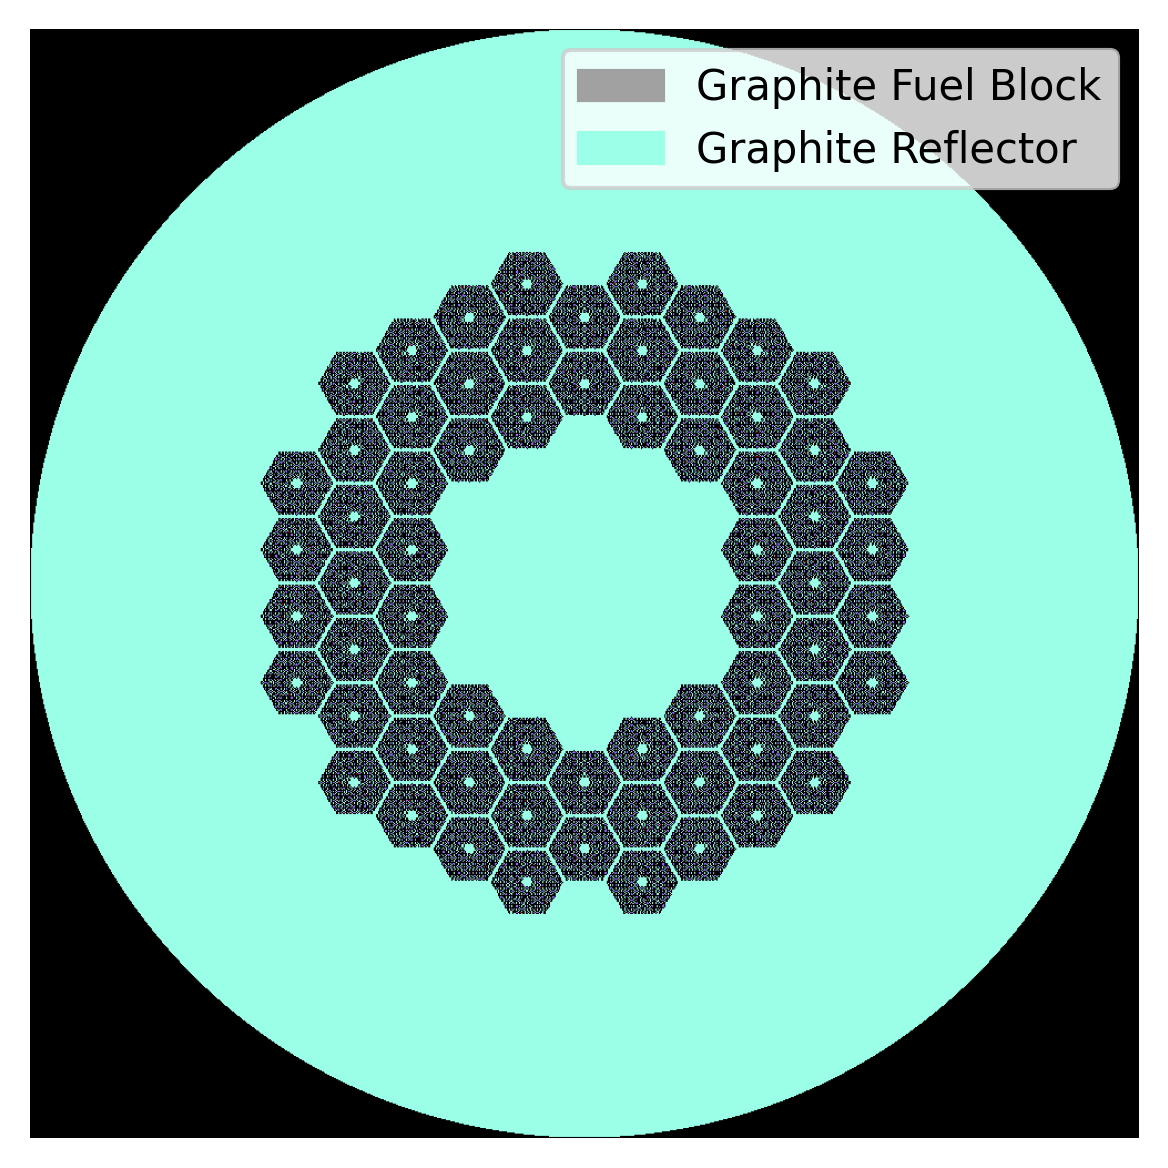
\includegraphics[width=\linewidth]{figures-fullcore/oecd-fullcore}
		\caption{Serpent model geometry.}
	\end{subfigure}
	\begin{subfigure}[t]{0.4\textwidth}
		\centering
		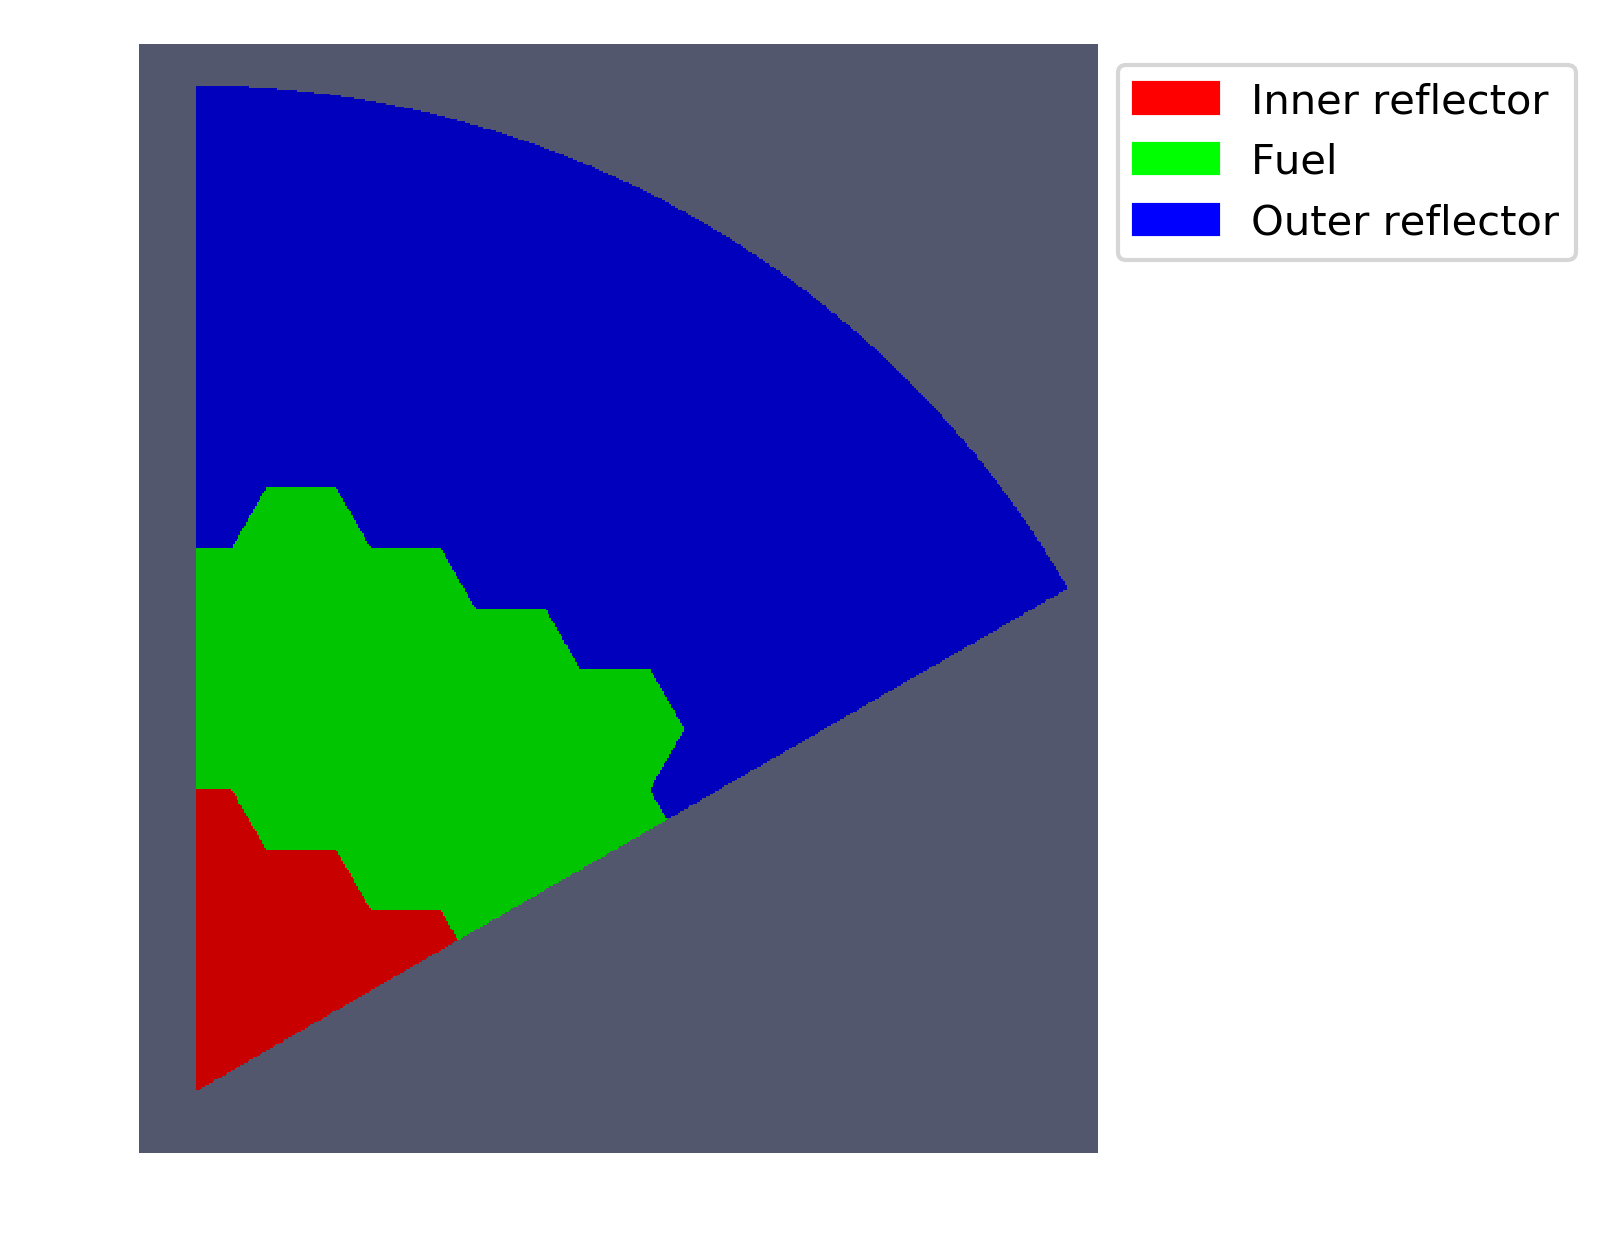
\includegraphics[width=\linewidth]{figures-fullcore/3D-fullcore-60-homo-meshB2}
		\caption{1/6$^{th}$ geometry for Moltres.}
	\end{subfigure}
	\hfill
	\caption{MHTGR-350 full core models.}
	\label{fig:fullcoremodel}
\end{figure}

%Power distribution at 600K
\begin{figure}[htbp!]
	\centering
	\begin{subfigure}[t]{0.4\textwidth}
		\centering
		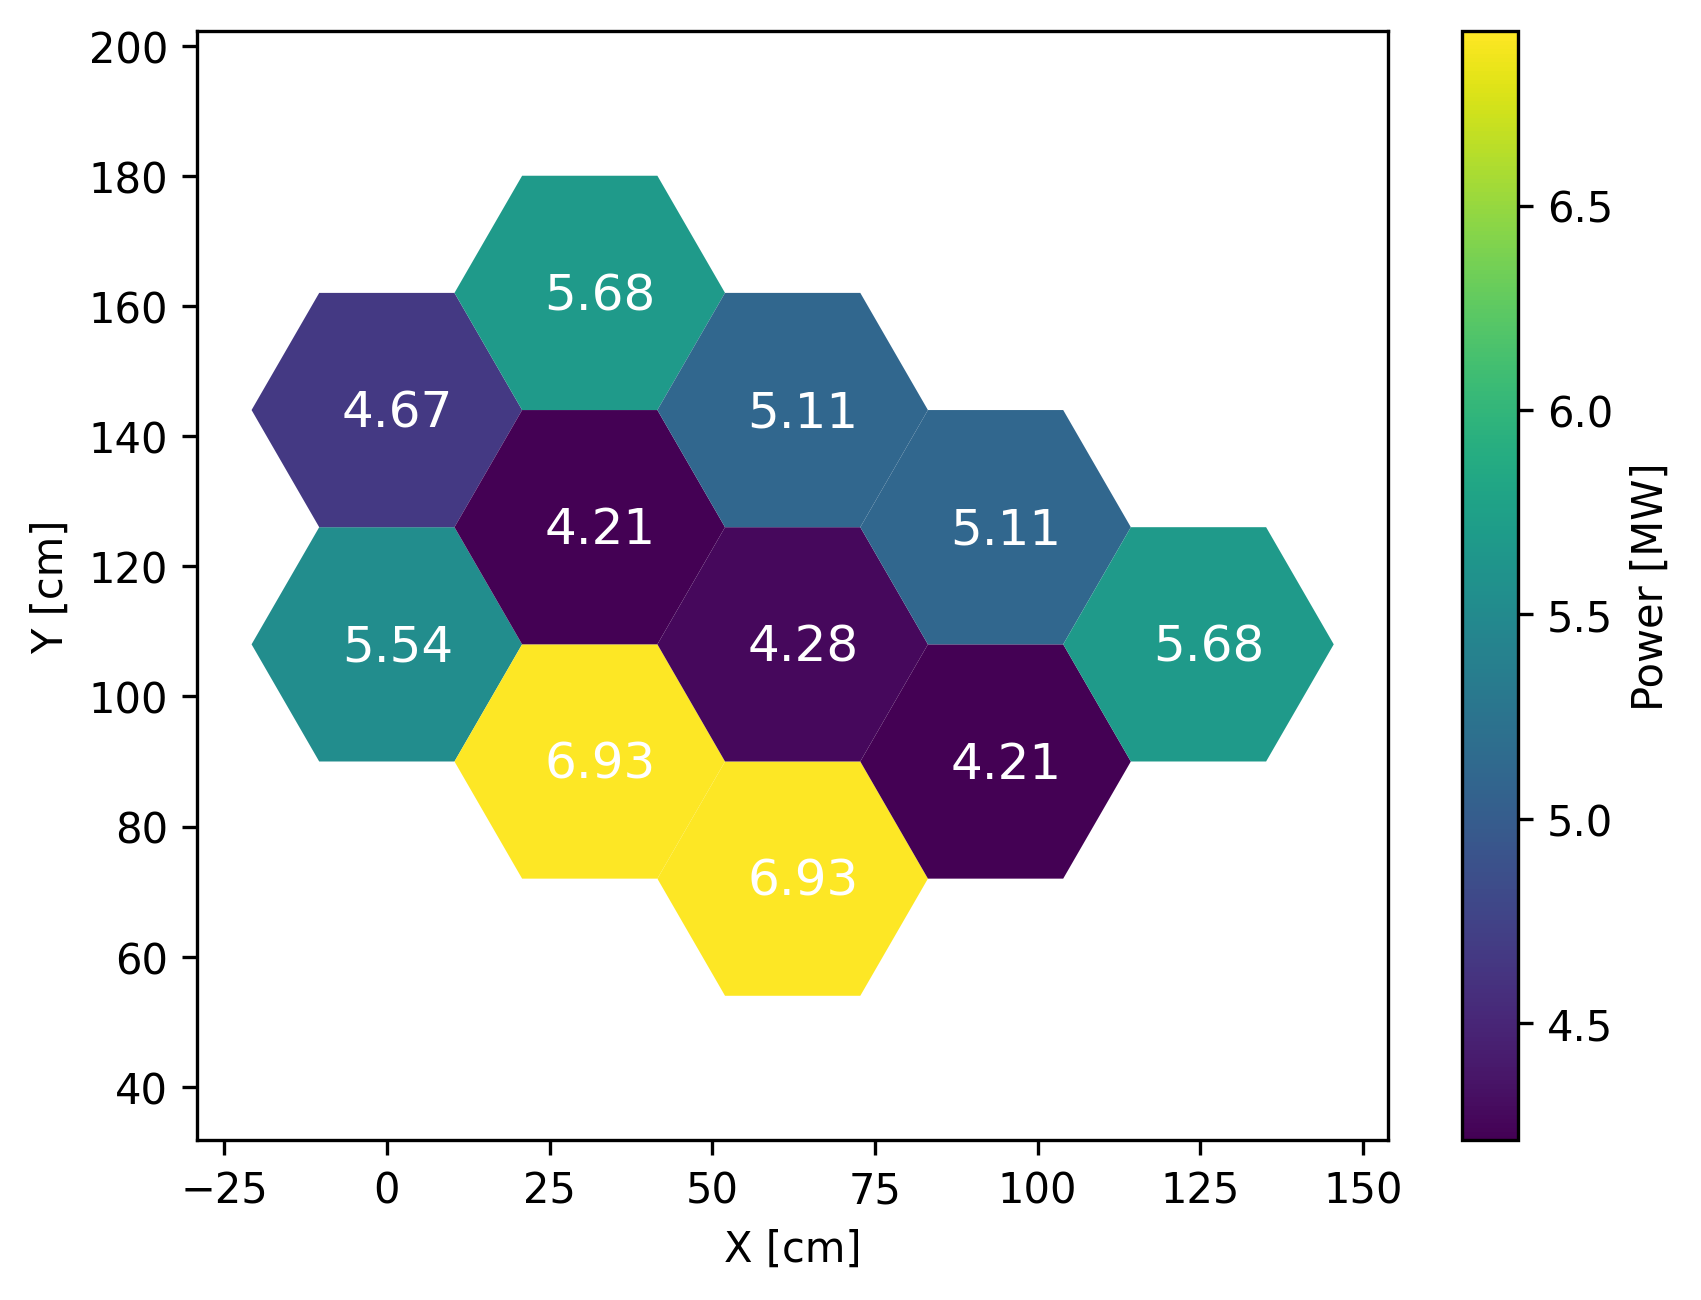
\includegraphics[width=\linewidth]{figures-fullcore/3D-fullcore-600-15Gd-power}
		\caption{Moltres.}
	\end{subfigure}
	\begin{subfigure}[t]{0.4\textwidth}
		\centering
		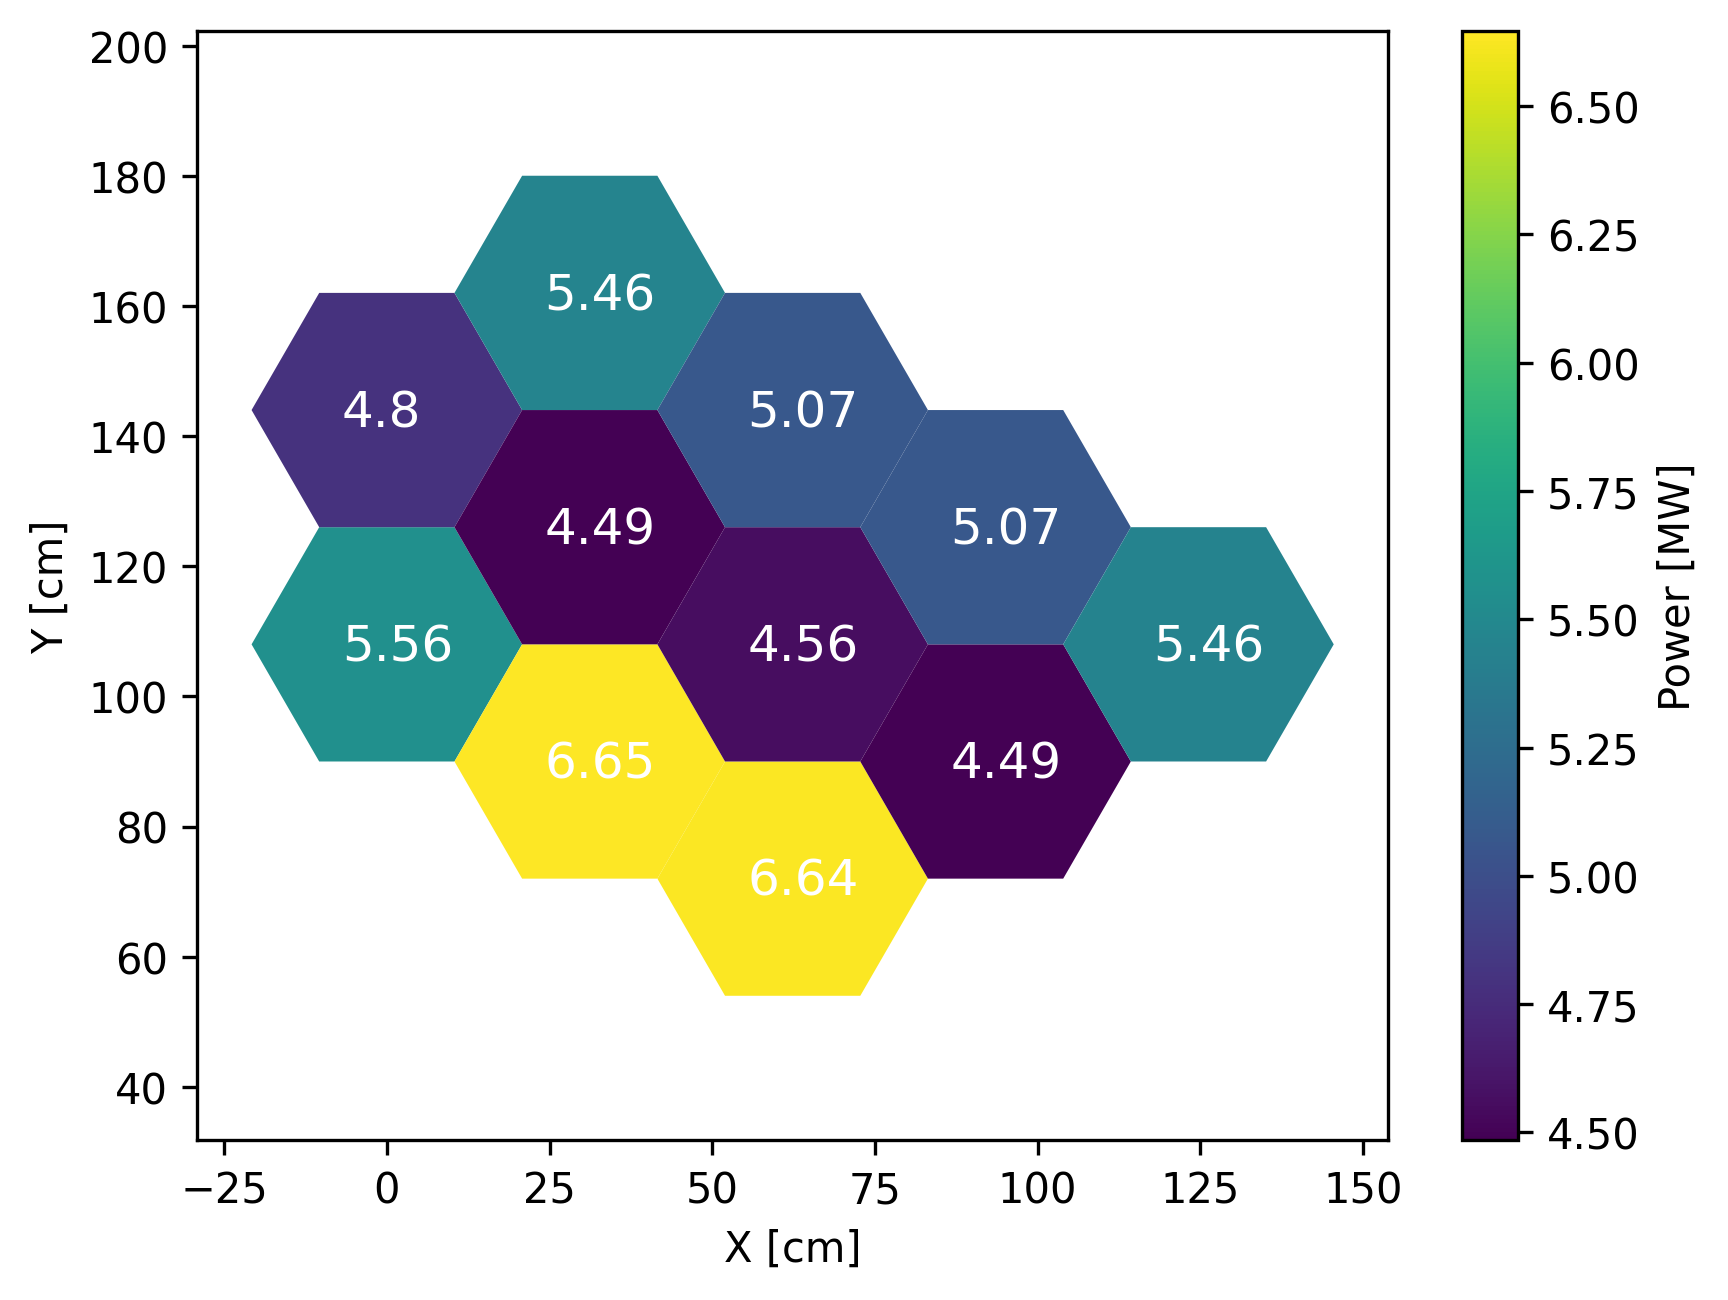
\includegraphics[width=\linewidth]{figures-fullcore/serpent26G-600-power}
		\caption{Serpent.}
	\end{subfigure}
	\hfill
	\caption{Radial power distribution at 600 K.}
	\label{fig:fullcore-600-power}
\end{figure}

%Power distribution at 1200K
\begin{figure}[htbp!]
	\centering
	\begin{subfigure}[t]{0.4\textwidth}
		\centering
		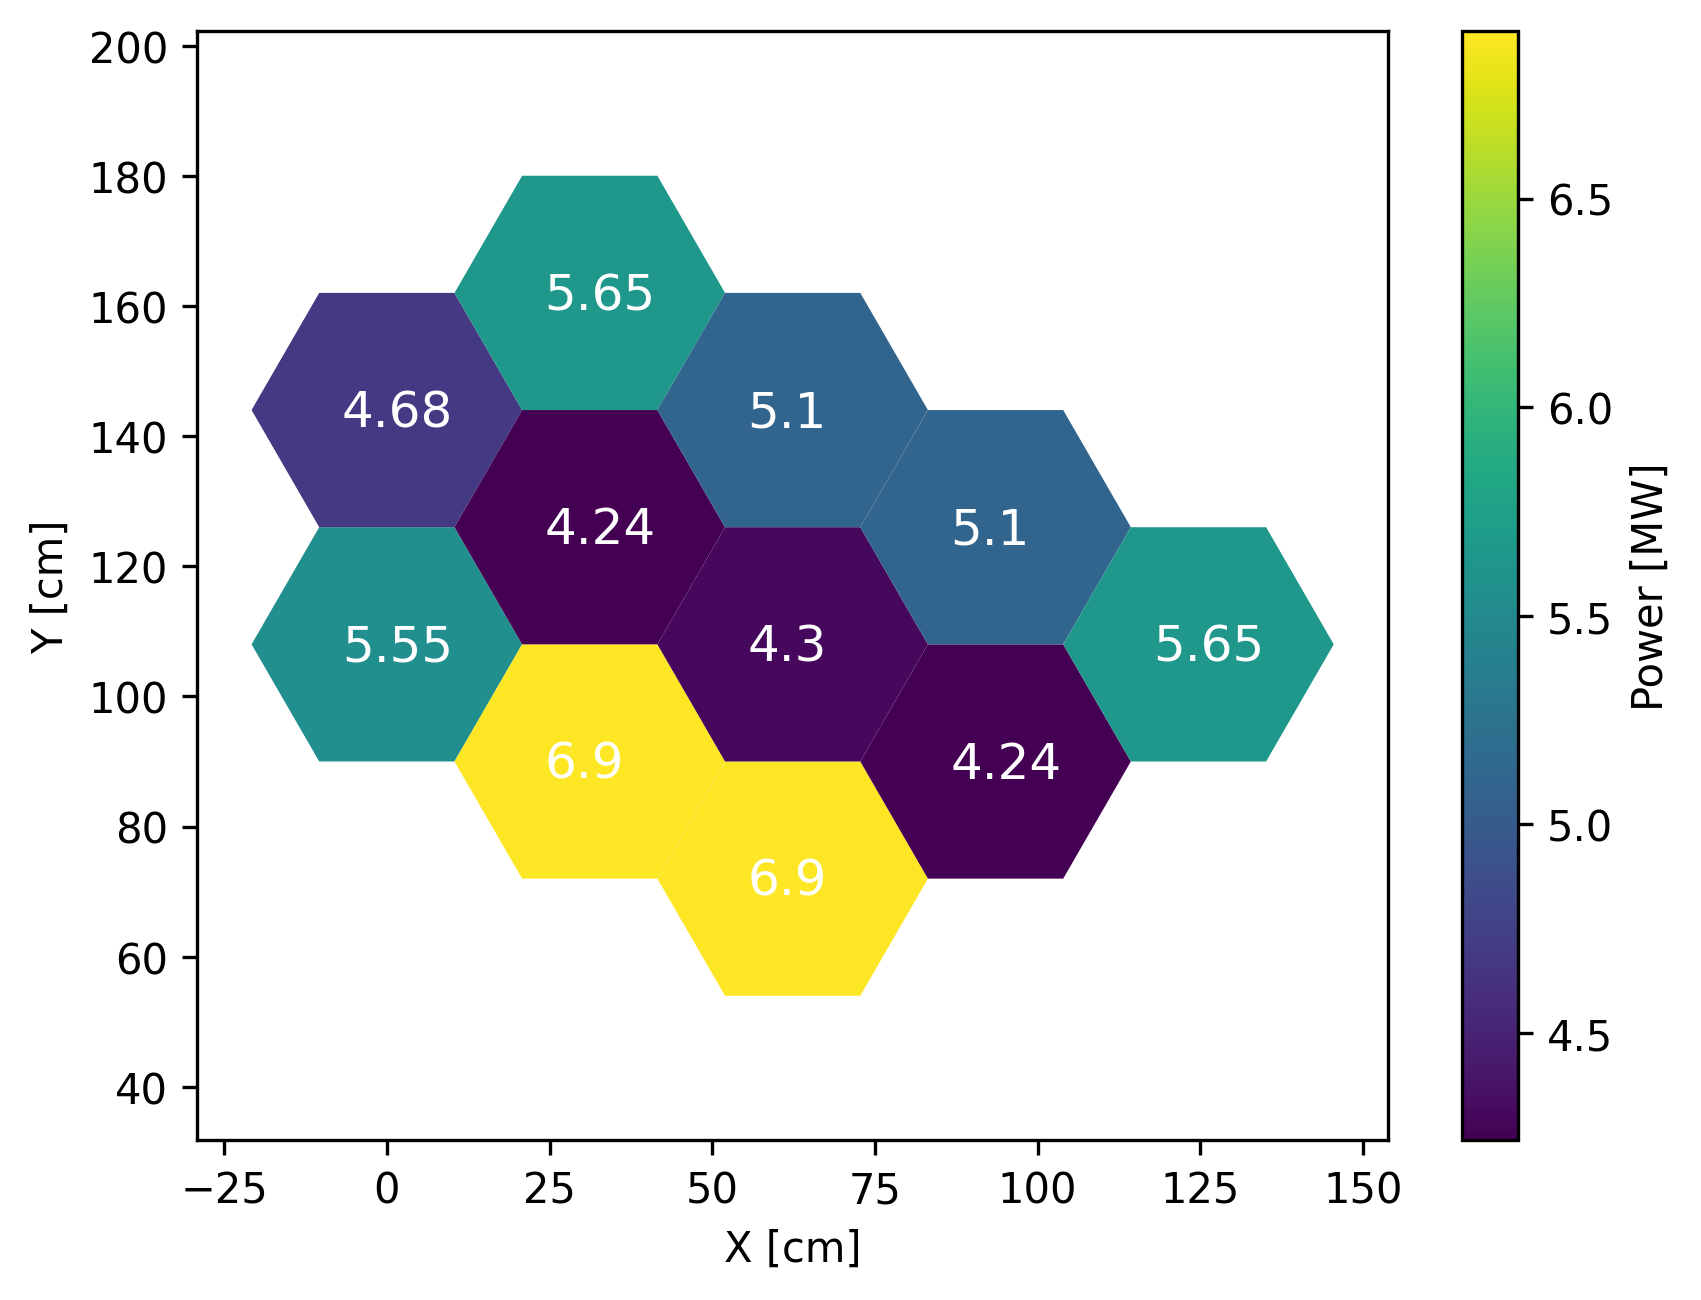
\includegraphics[width=\linewidth]{figures-fullcore/3D-fullcore-1200-15Gc-power}
		\caption{Moltres.}
	\end{subfigure}
	\begin{subfigure}[t]{0.4\textwidth}
		\centering
		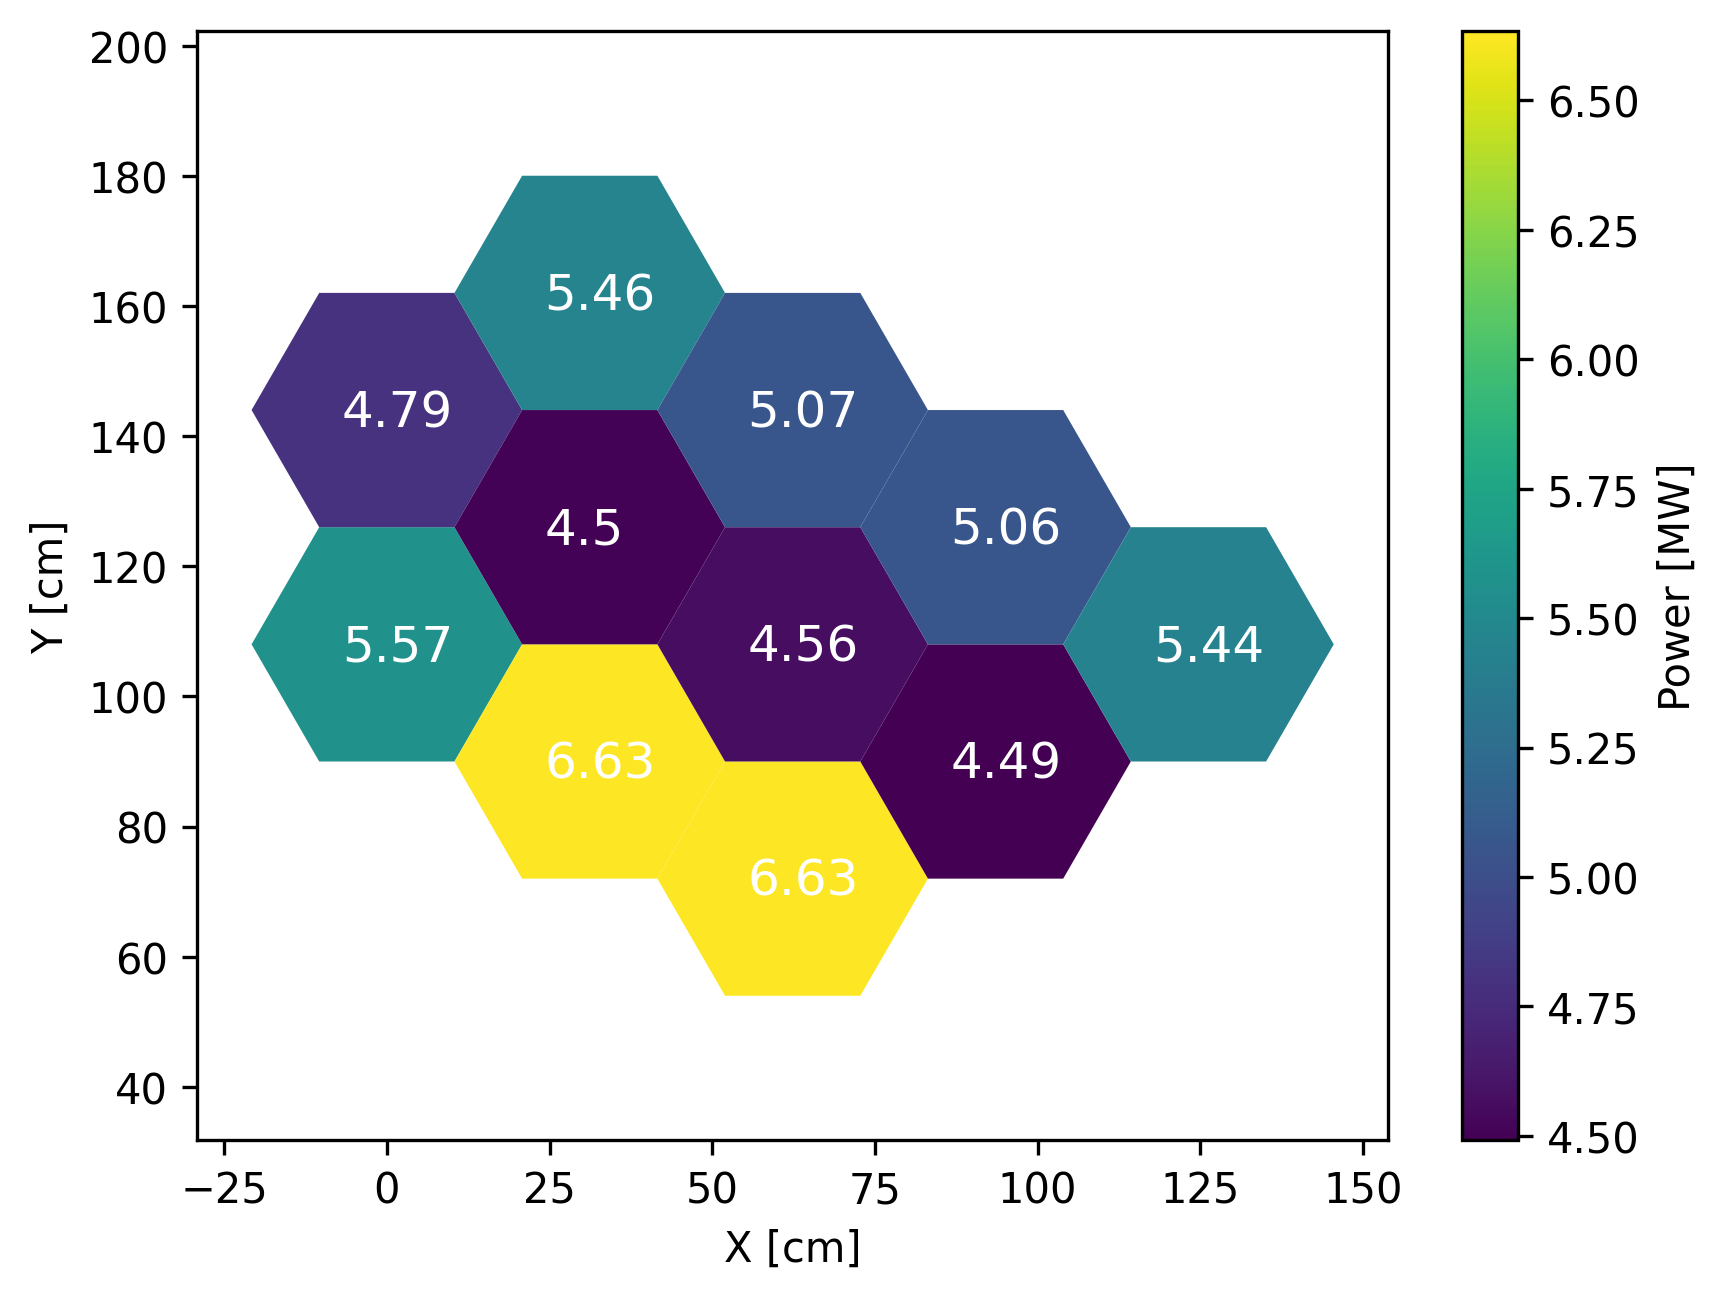
\includegraphics[width=\linewidth]{figures-fullcore/serpent26G-1200-power}
		\caption{Serpent.}
	\end{subfigure}
	\hfill
	\caption{Radial power distribution.}
	\label{fig:fullcore-1200-power}
\end{figure}

%Detectors
\begin{figure}[htbp!]
	\centering
	\begin{subfigure}[t]{0.4\textwidth}
		\centering
		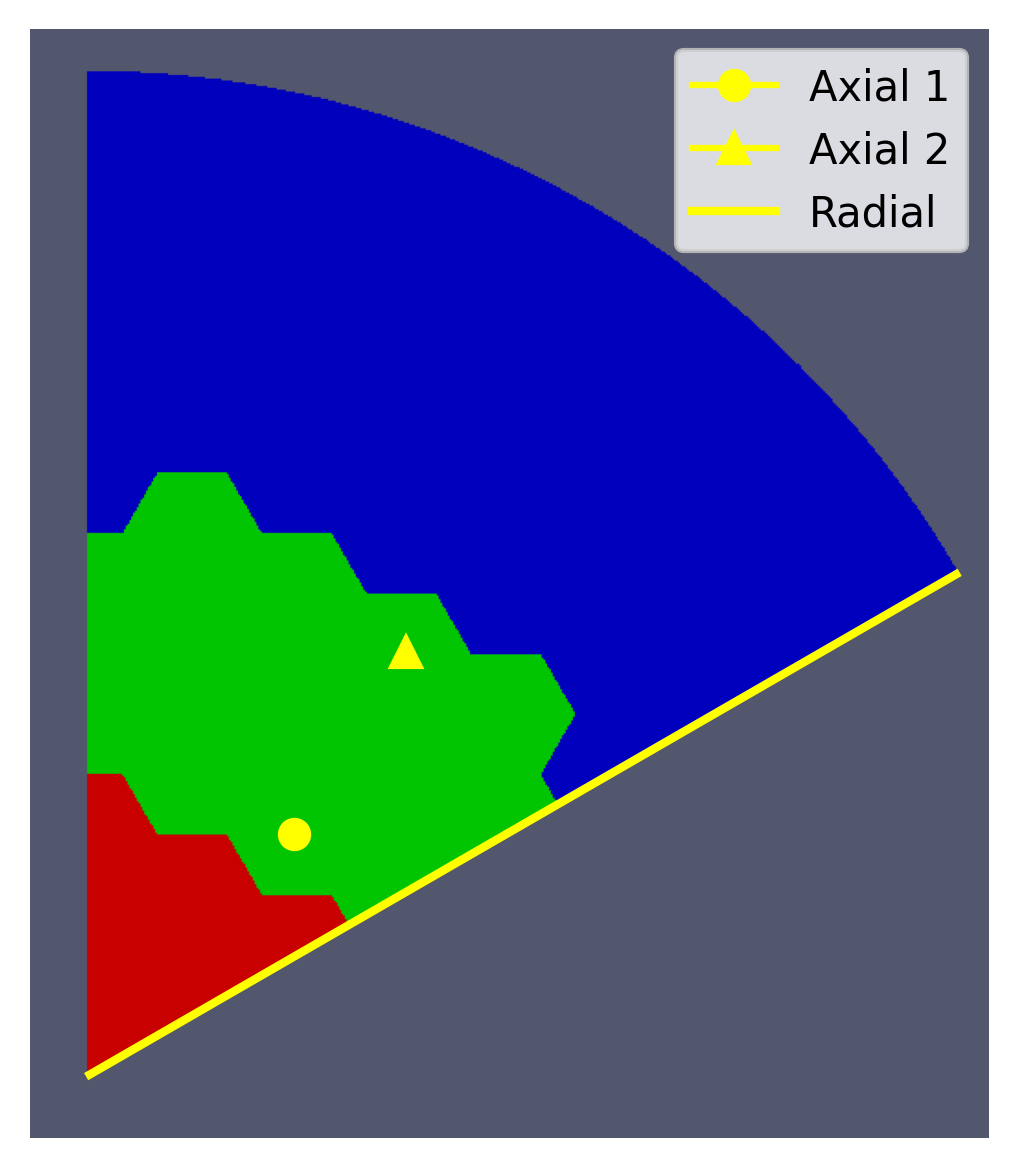
\includegraphics[width=\linewidth]{figures-fullcore/3D-fullcore-60-detectors}
		\caption{Moltres.}
	\end{subfigure}
	\begin{subfigure}[t]{0.4\textwidth}
		\centering
		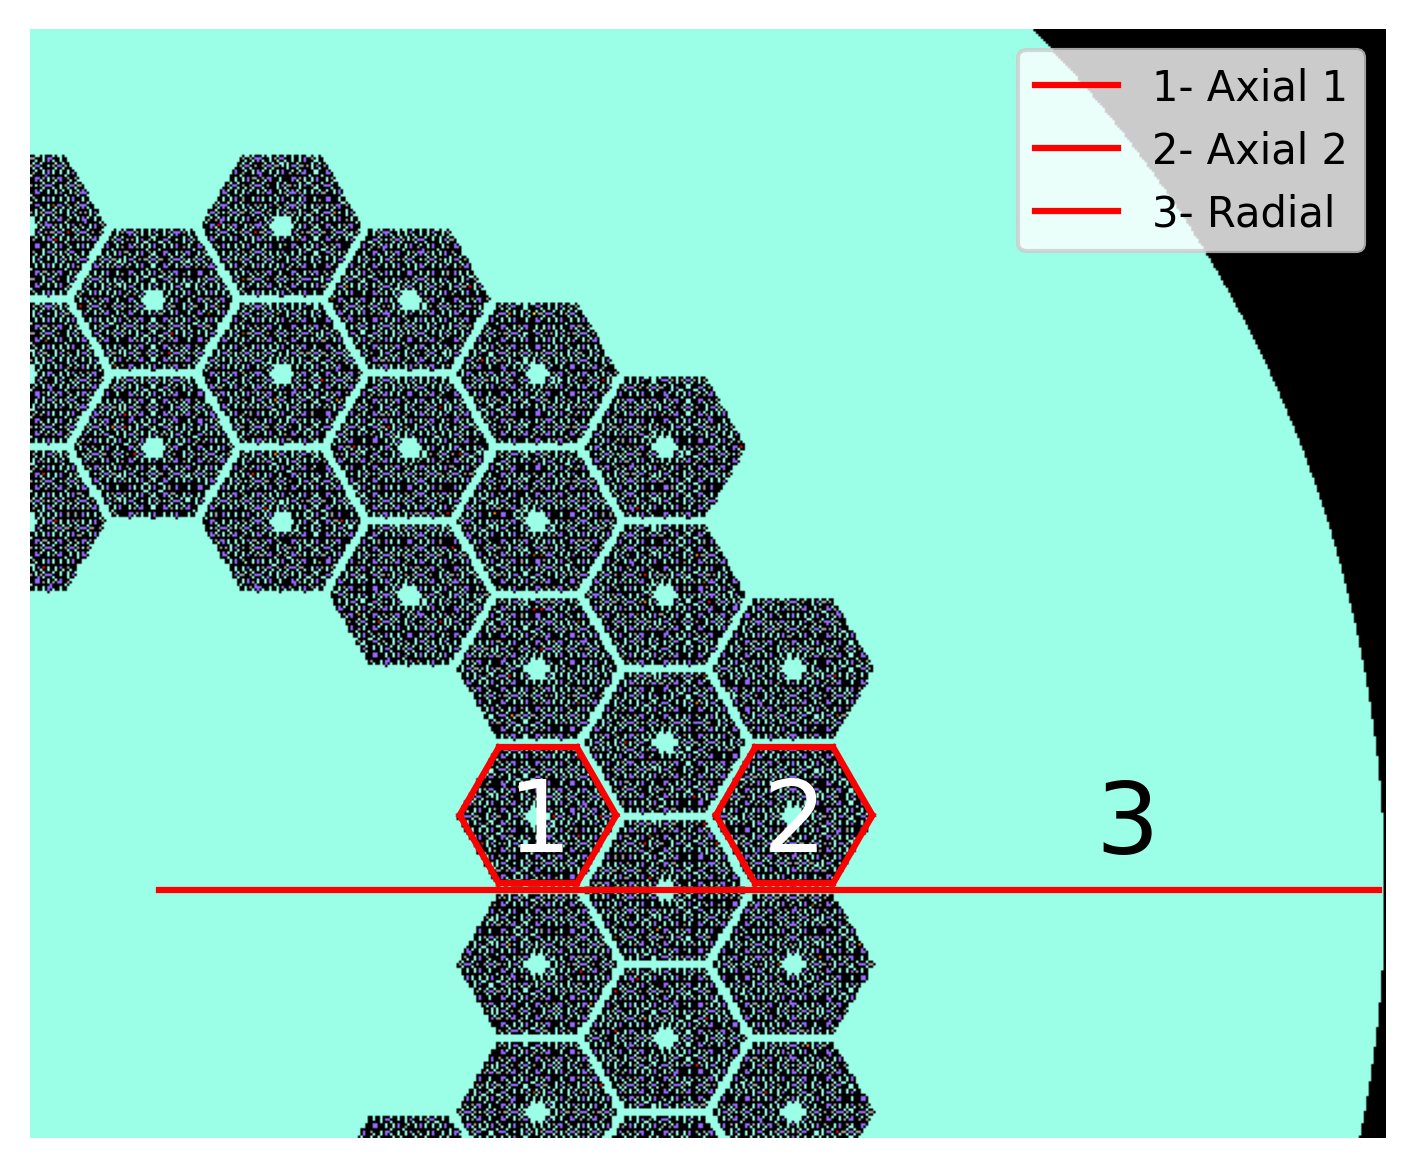
\includegraphics[width=\linewidth]{figures-fullcore/oecd-fullcore-detectorsB}
		\caption{Serpent.}
	\end{subfigure}
	\hfill
	\caption{Flux detector locations.}
	\label{fig:fullcore-detectors}
\end{figure}

%Axial flux1 at 600K
\begin{figure}[htbp!]
	\centering
	\begin{subfigure}[t]{0.4\textwidth}
		\centering
		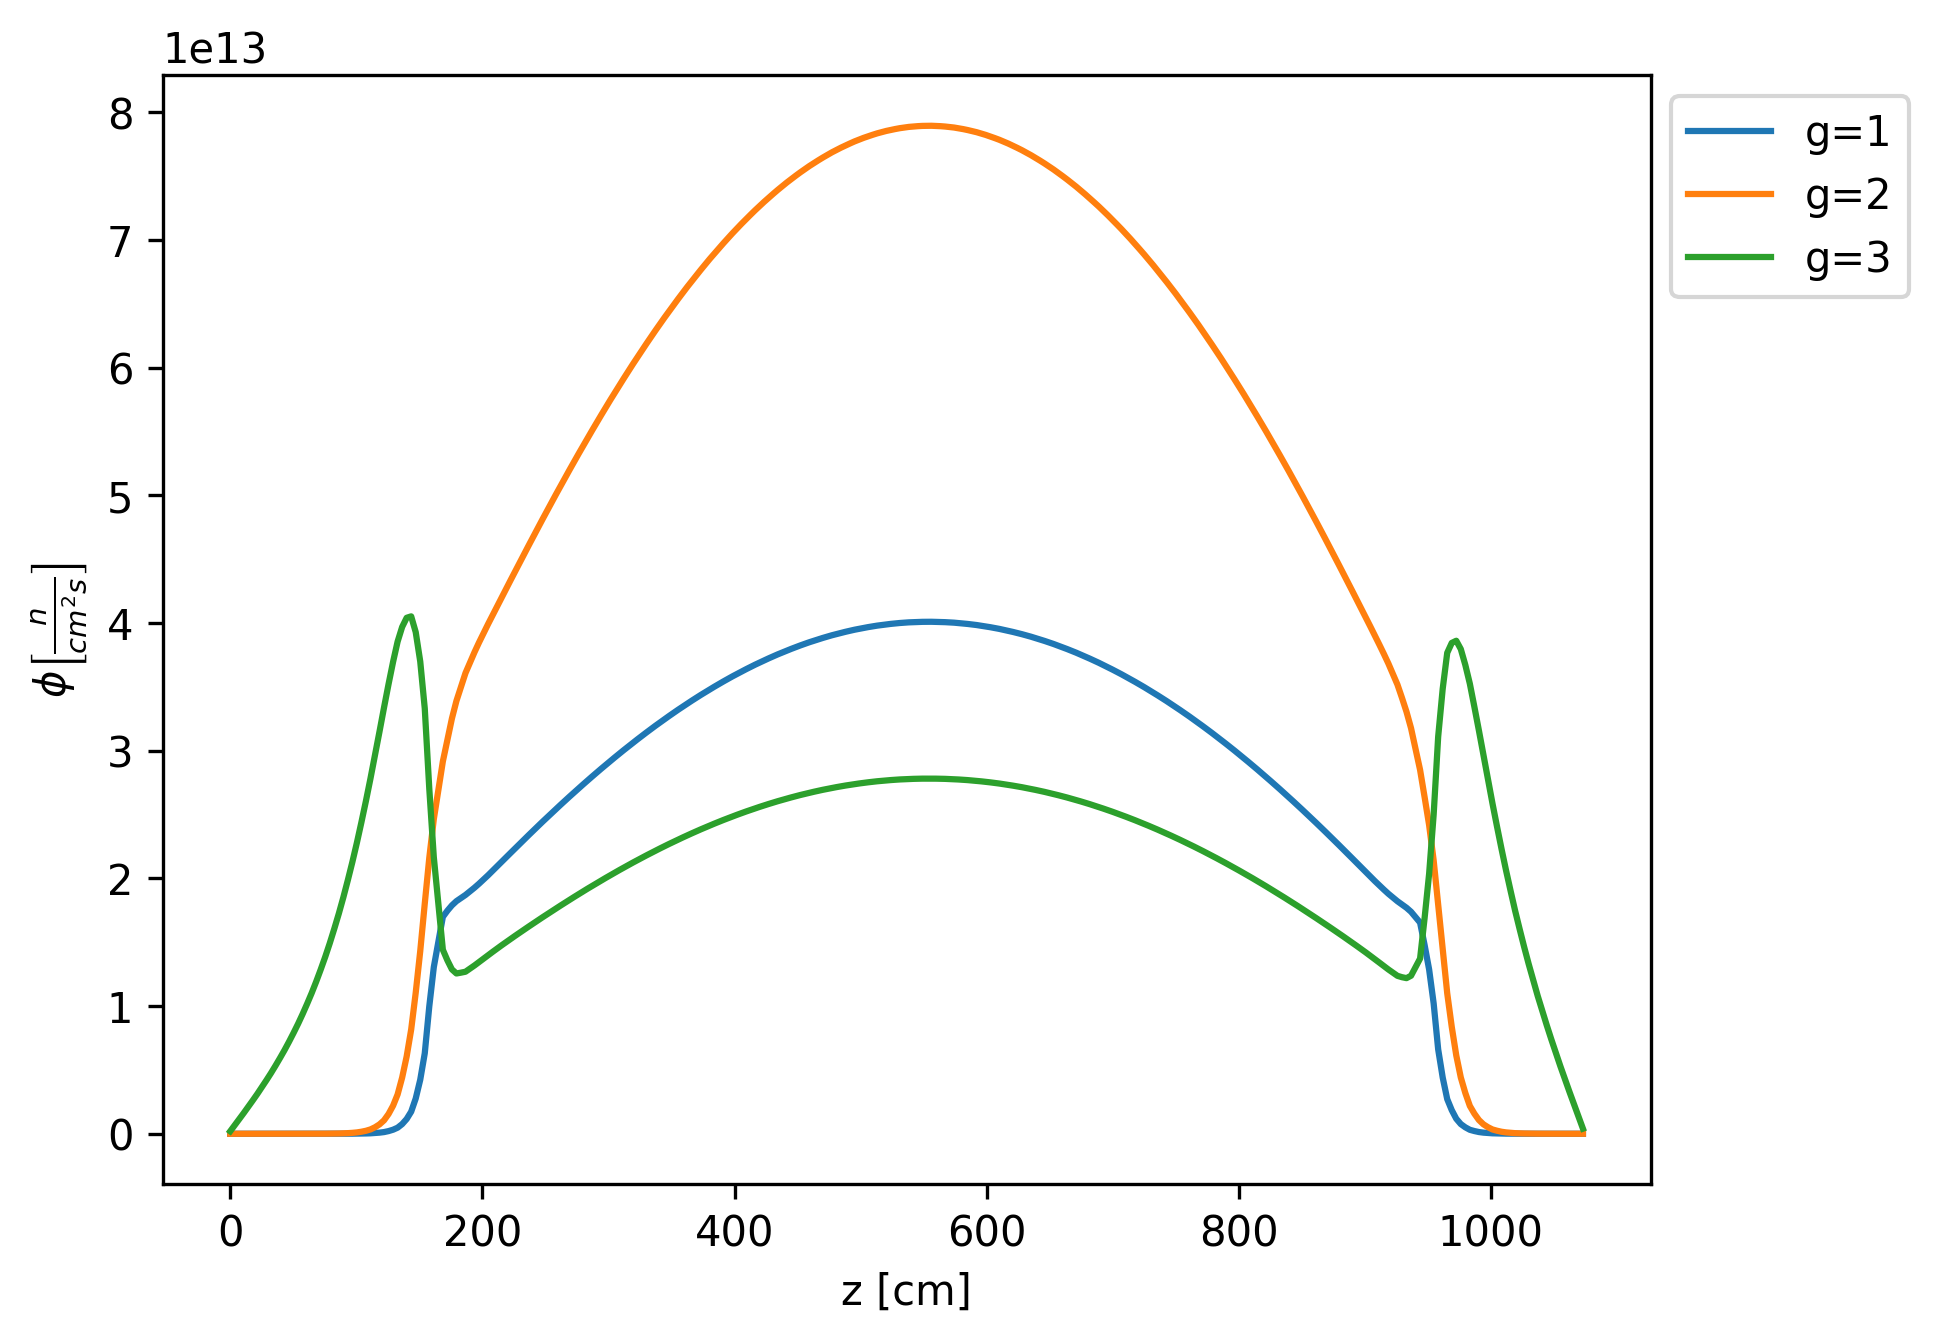
\includegraphics[width=\linewidth]{figures-fullcore/3D-fullcore-600-15Gd-axial1}
		\caption{Moltres.}
	\end{subfigure}
	\begin{subfigure}[t]{0.4\textwidth}
		\centering
		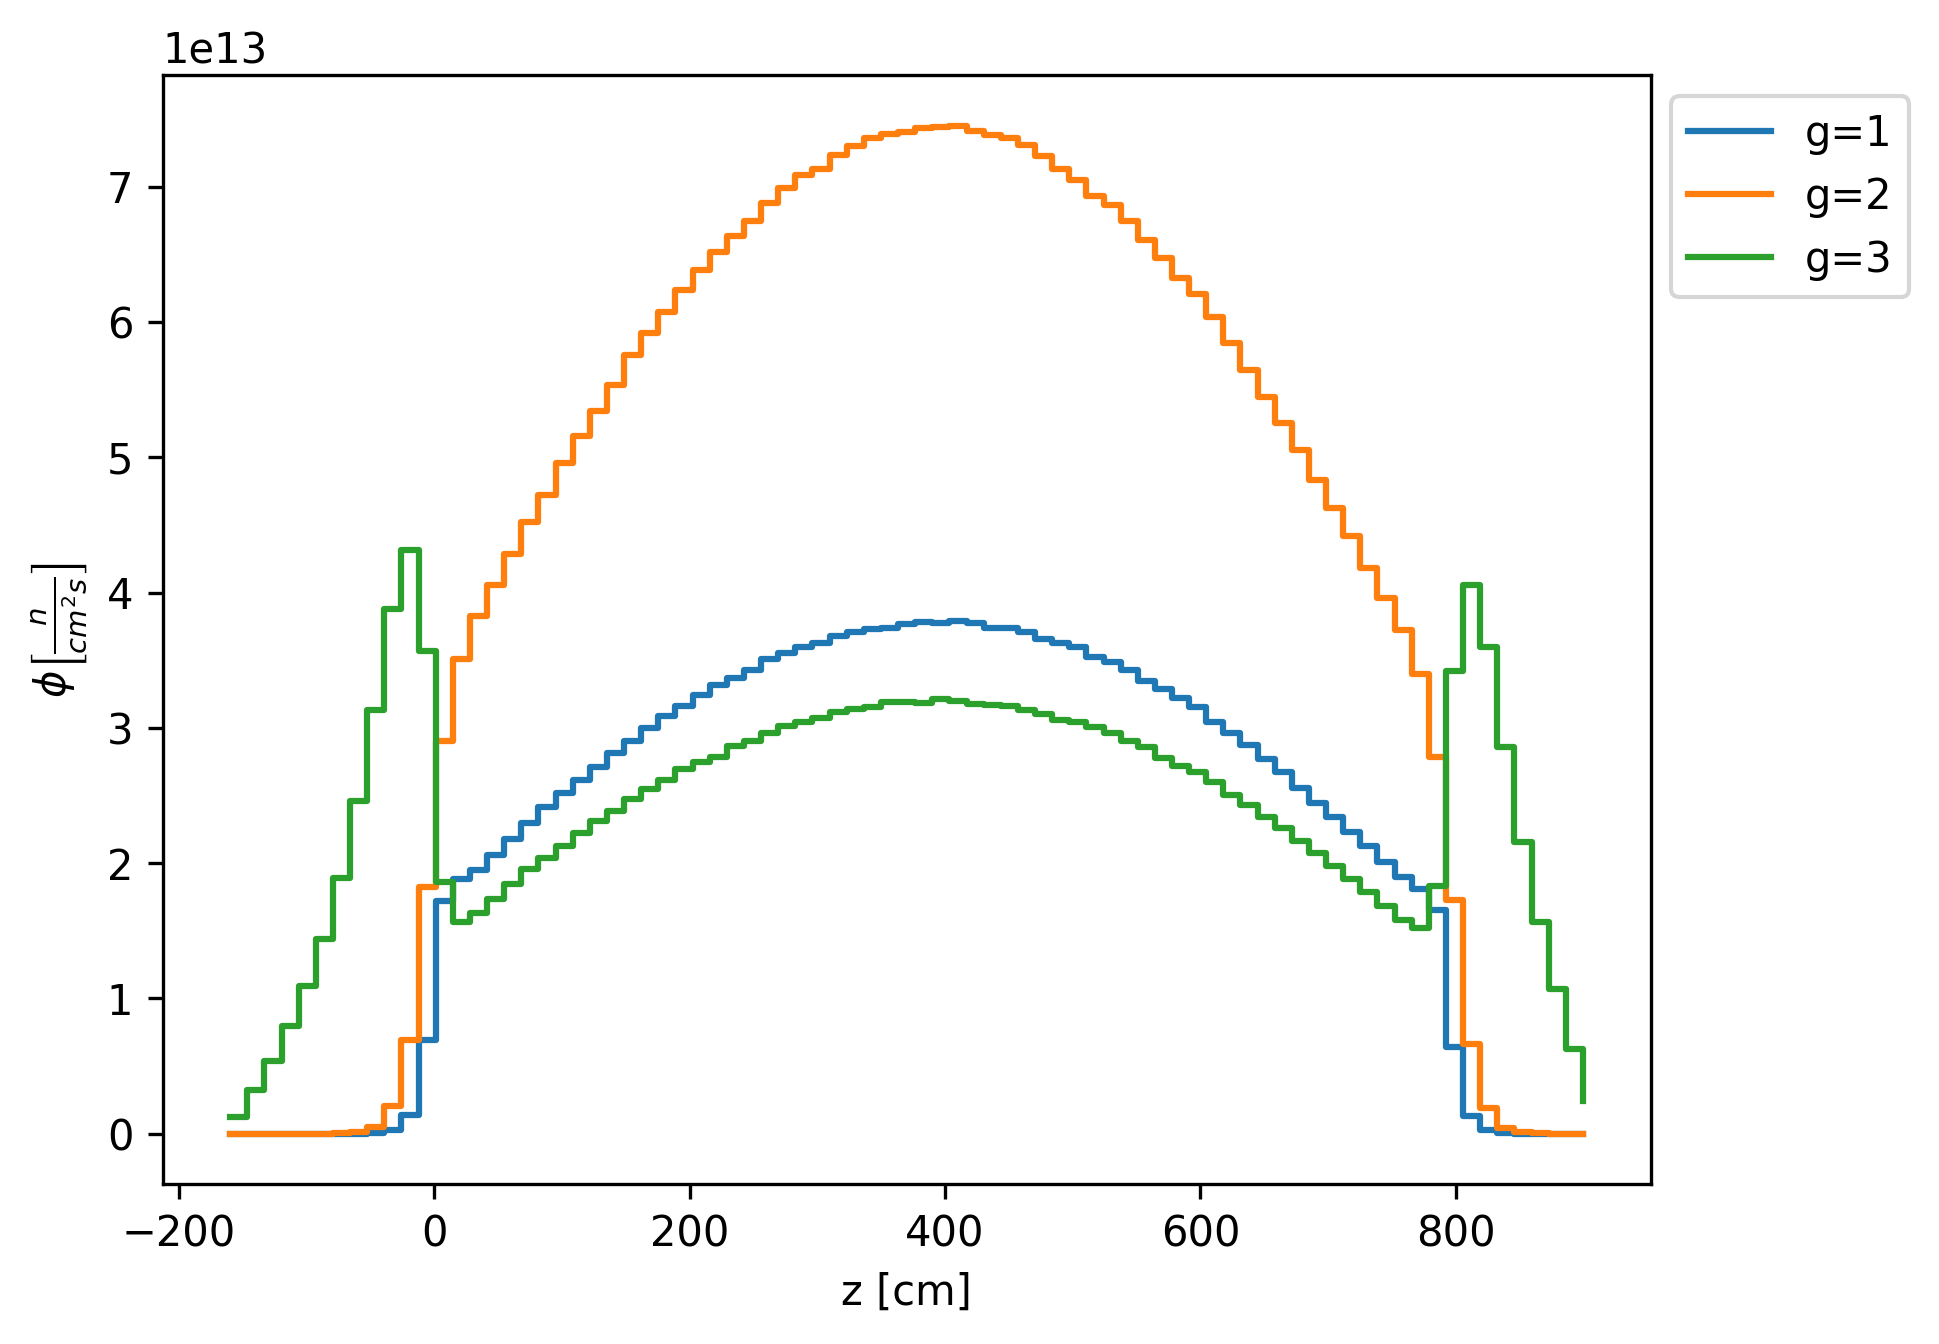
\includegraphics[width=\linewidth]{figures-fullcore/serpent26G-600-collapse-Axial1}
		\caption{Serpent.}
	\end{subfigure}
	\hfill
	\caption{Flux in axial detector 1 at 600 K.}
	\label{fig:fullcore-600-axial1}
\end{figure}

%Axial flux3
\begin{figure}[htbp!]
	\centering
	\begin{subfigure}[t]{0.4\textwidth}
		\centering
		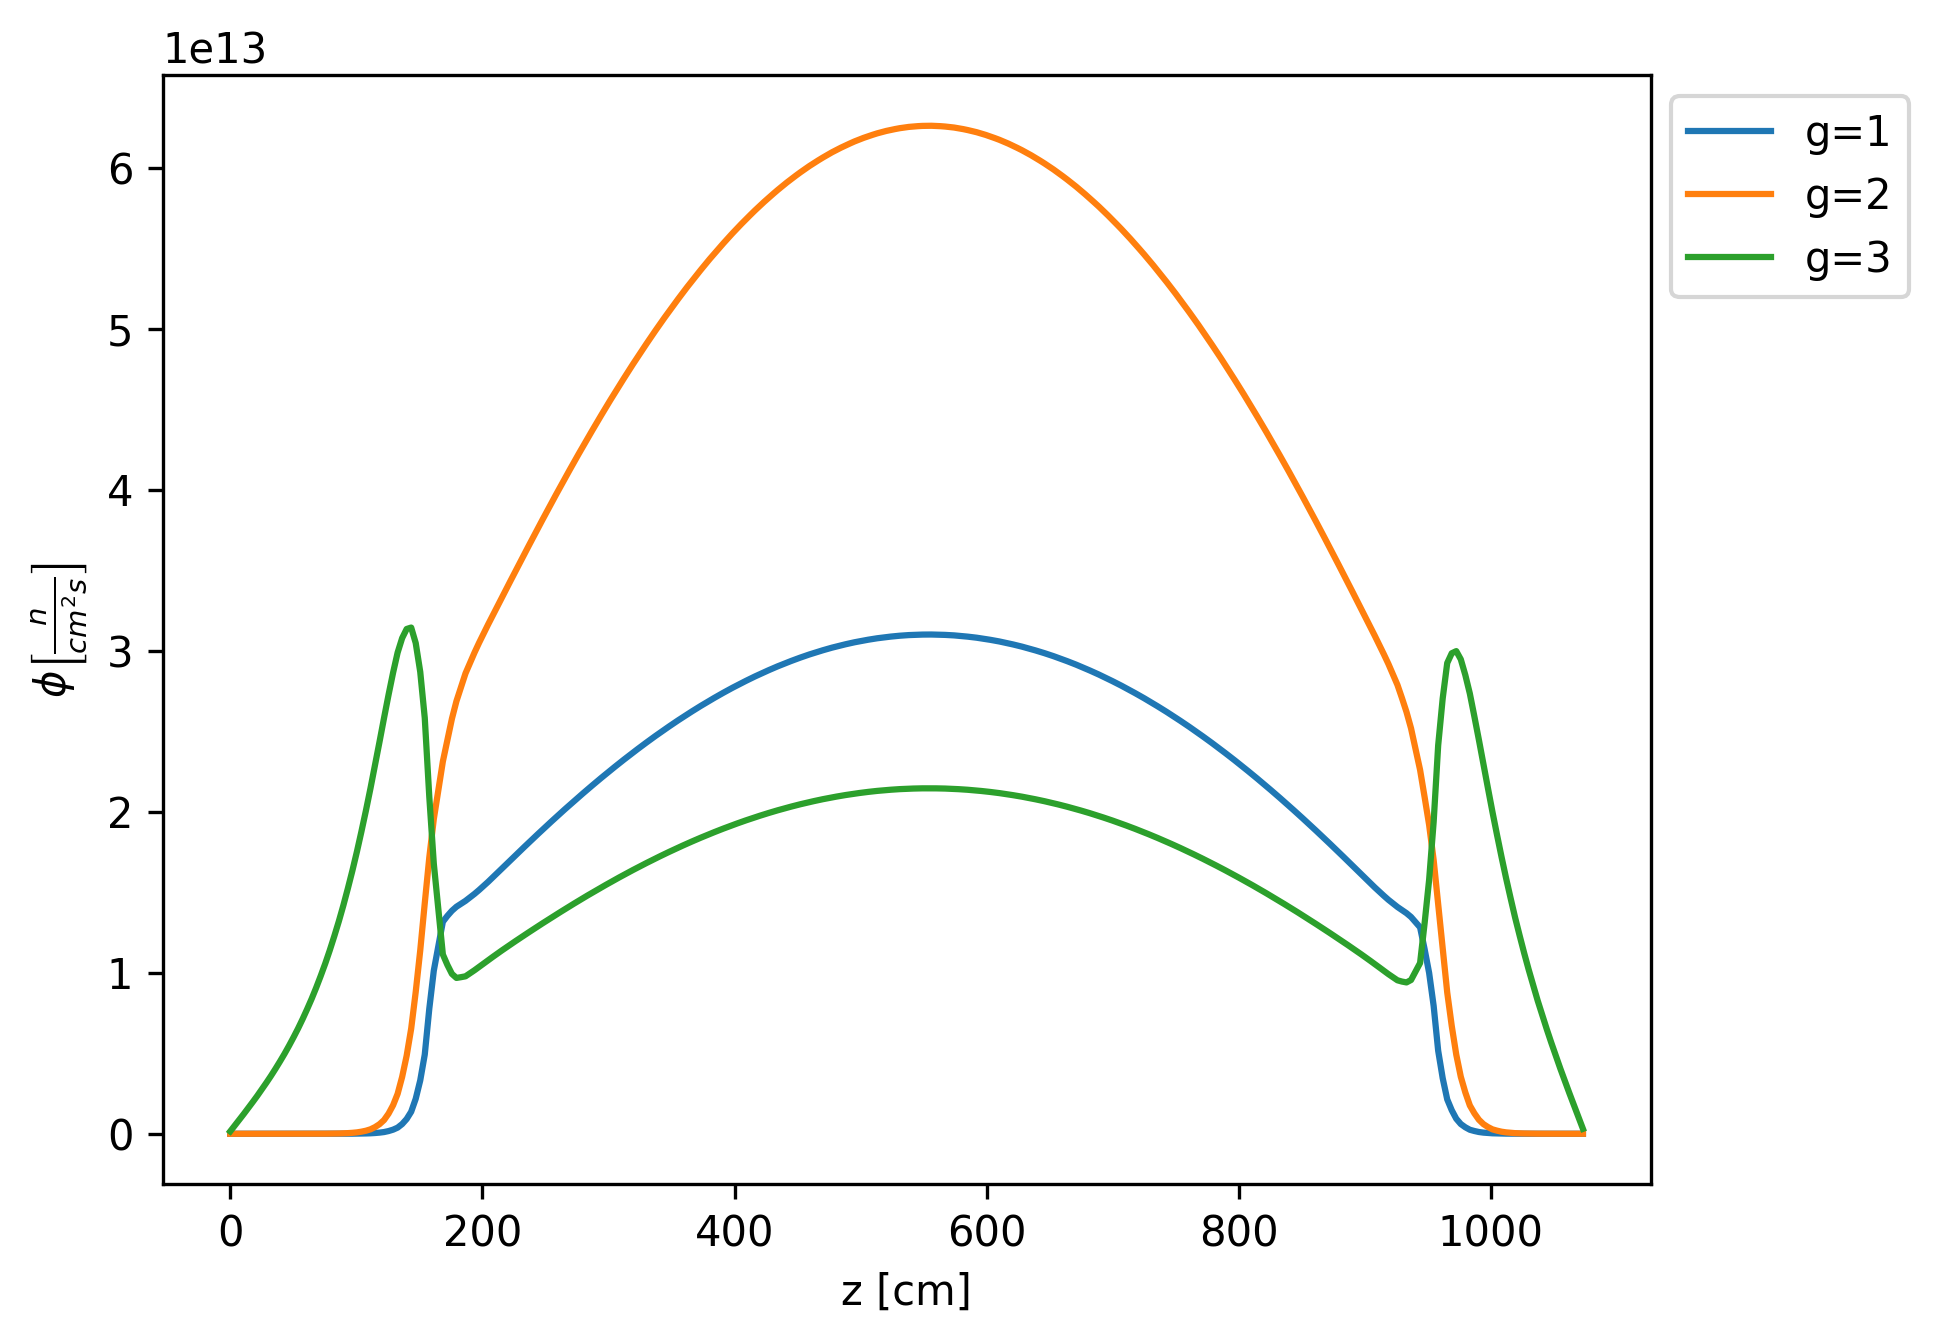
\includegraphics[width=\linewidth]{figures-fullcore/3D-fullcore-600-15Gd-axial3}
		\caption{Moltres.}
	\end{subfigure}
	\begin{subfigure}[t]{0.4\textwidth}
		\centering
		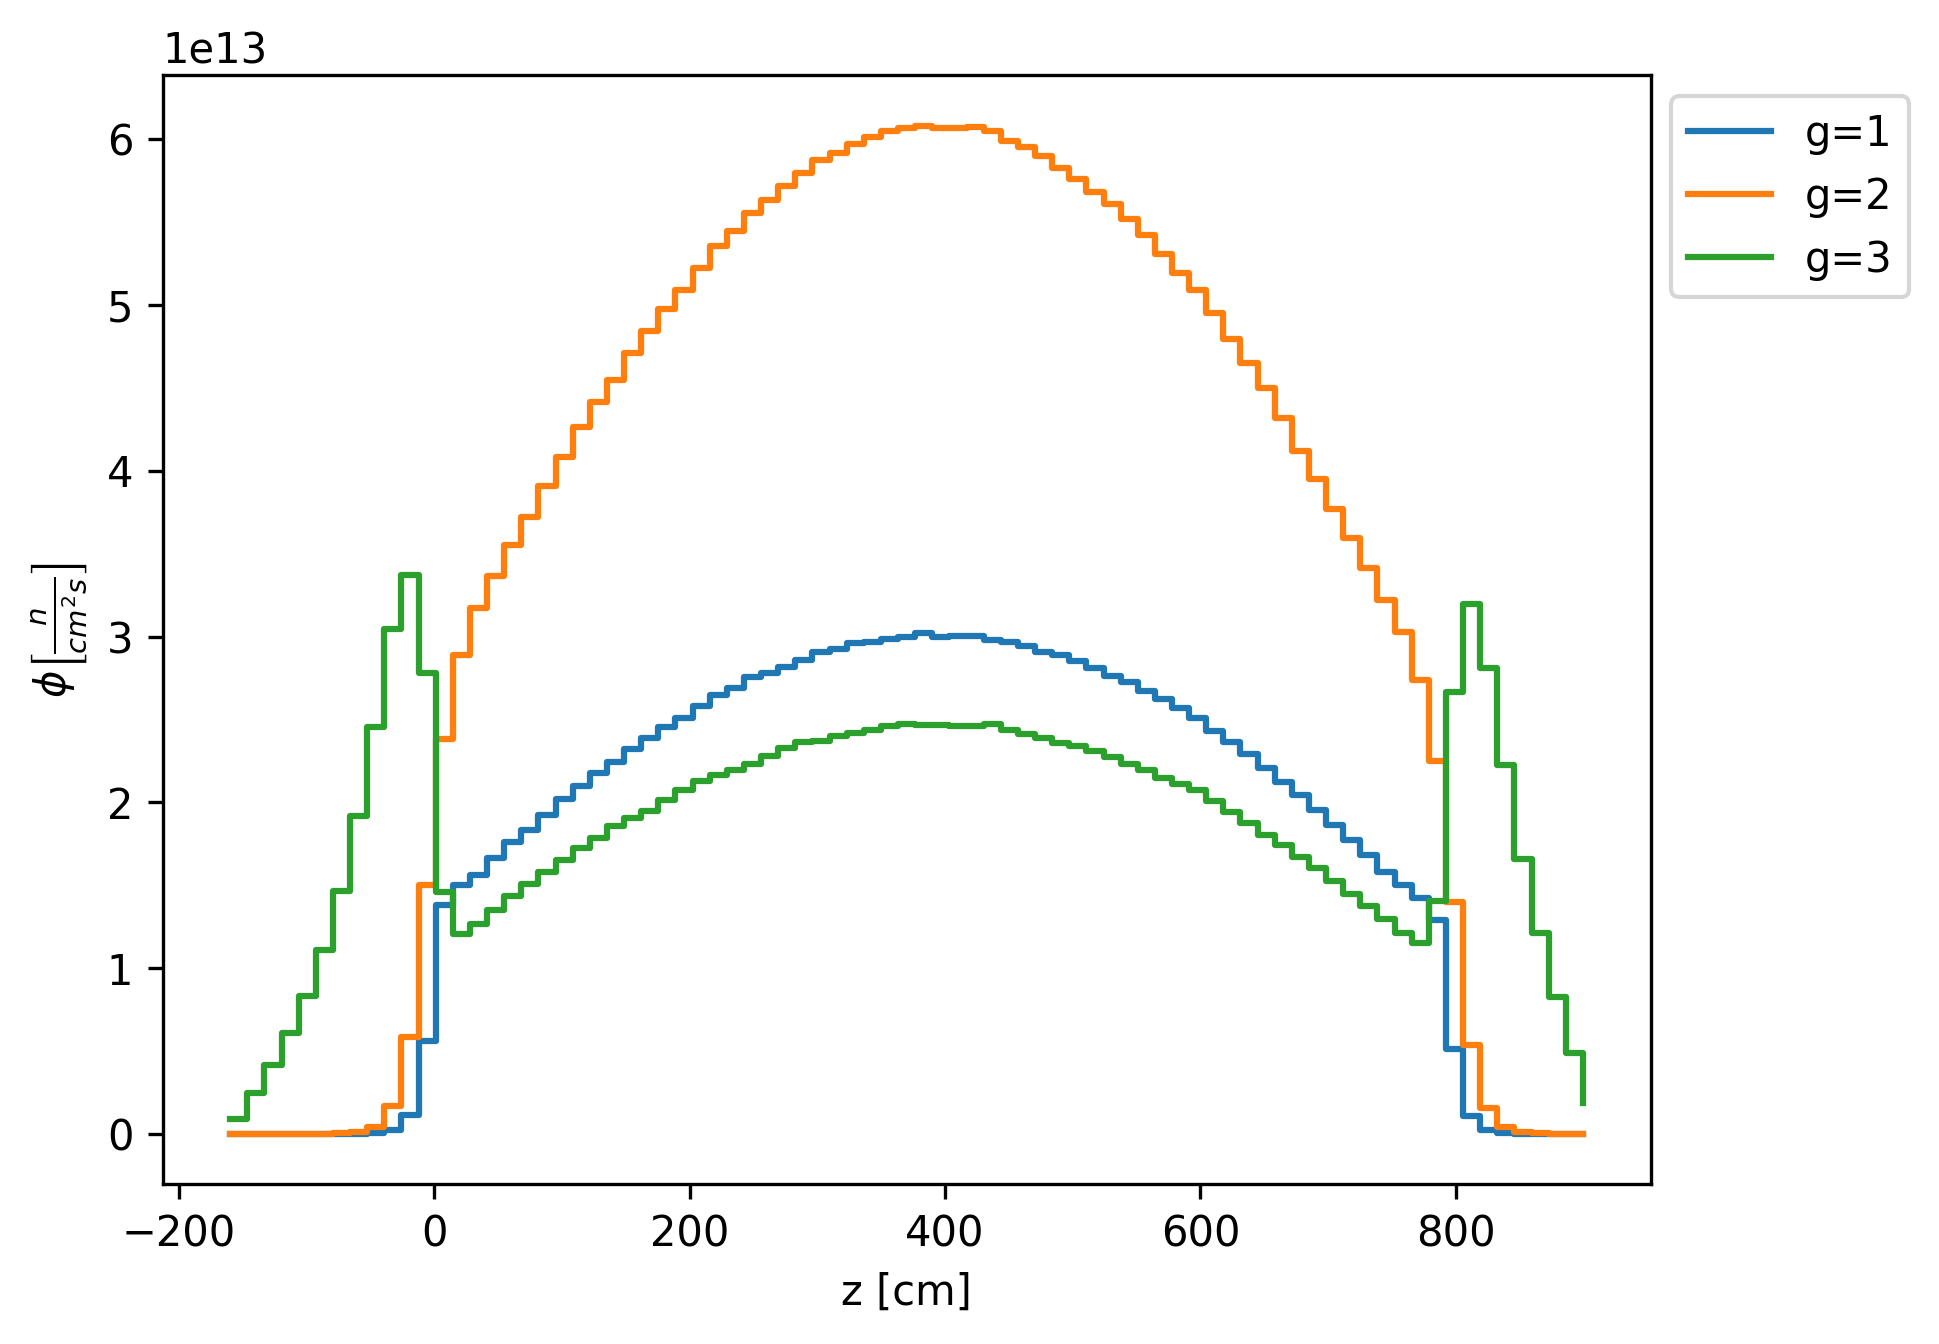
\includegraphics[width=\linewidth]{figures-fullcore/serpent26G-600-collapse-Axial2}
		\caption{Serpent.}
	\end{subfigure}
	\hfill
	\caption{Flux in axial detector 2 at 600 K.}
	\label{fig:fullcore-600-axial2}
\end{figure}

%Radial flux
\begin{figure}[htbp!]
	\centering
	\begin{subfigure}[t]{0.4\textwidth}
		\centering
		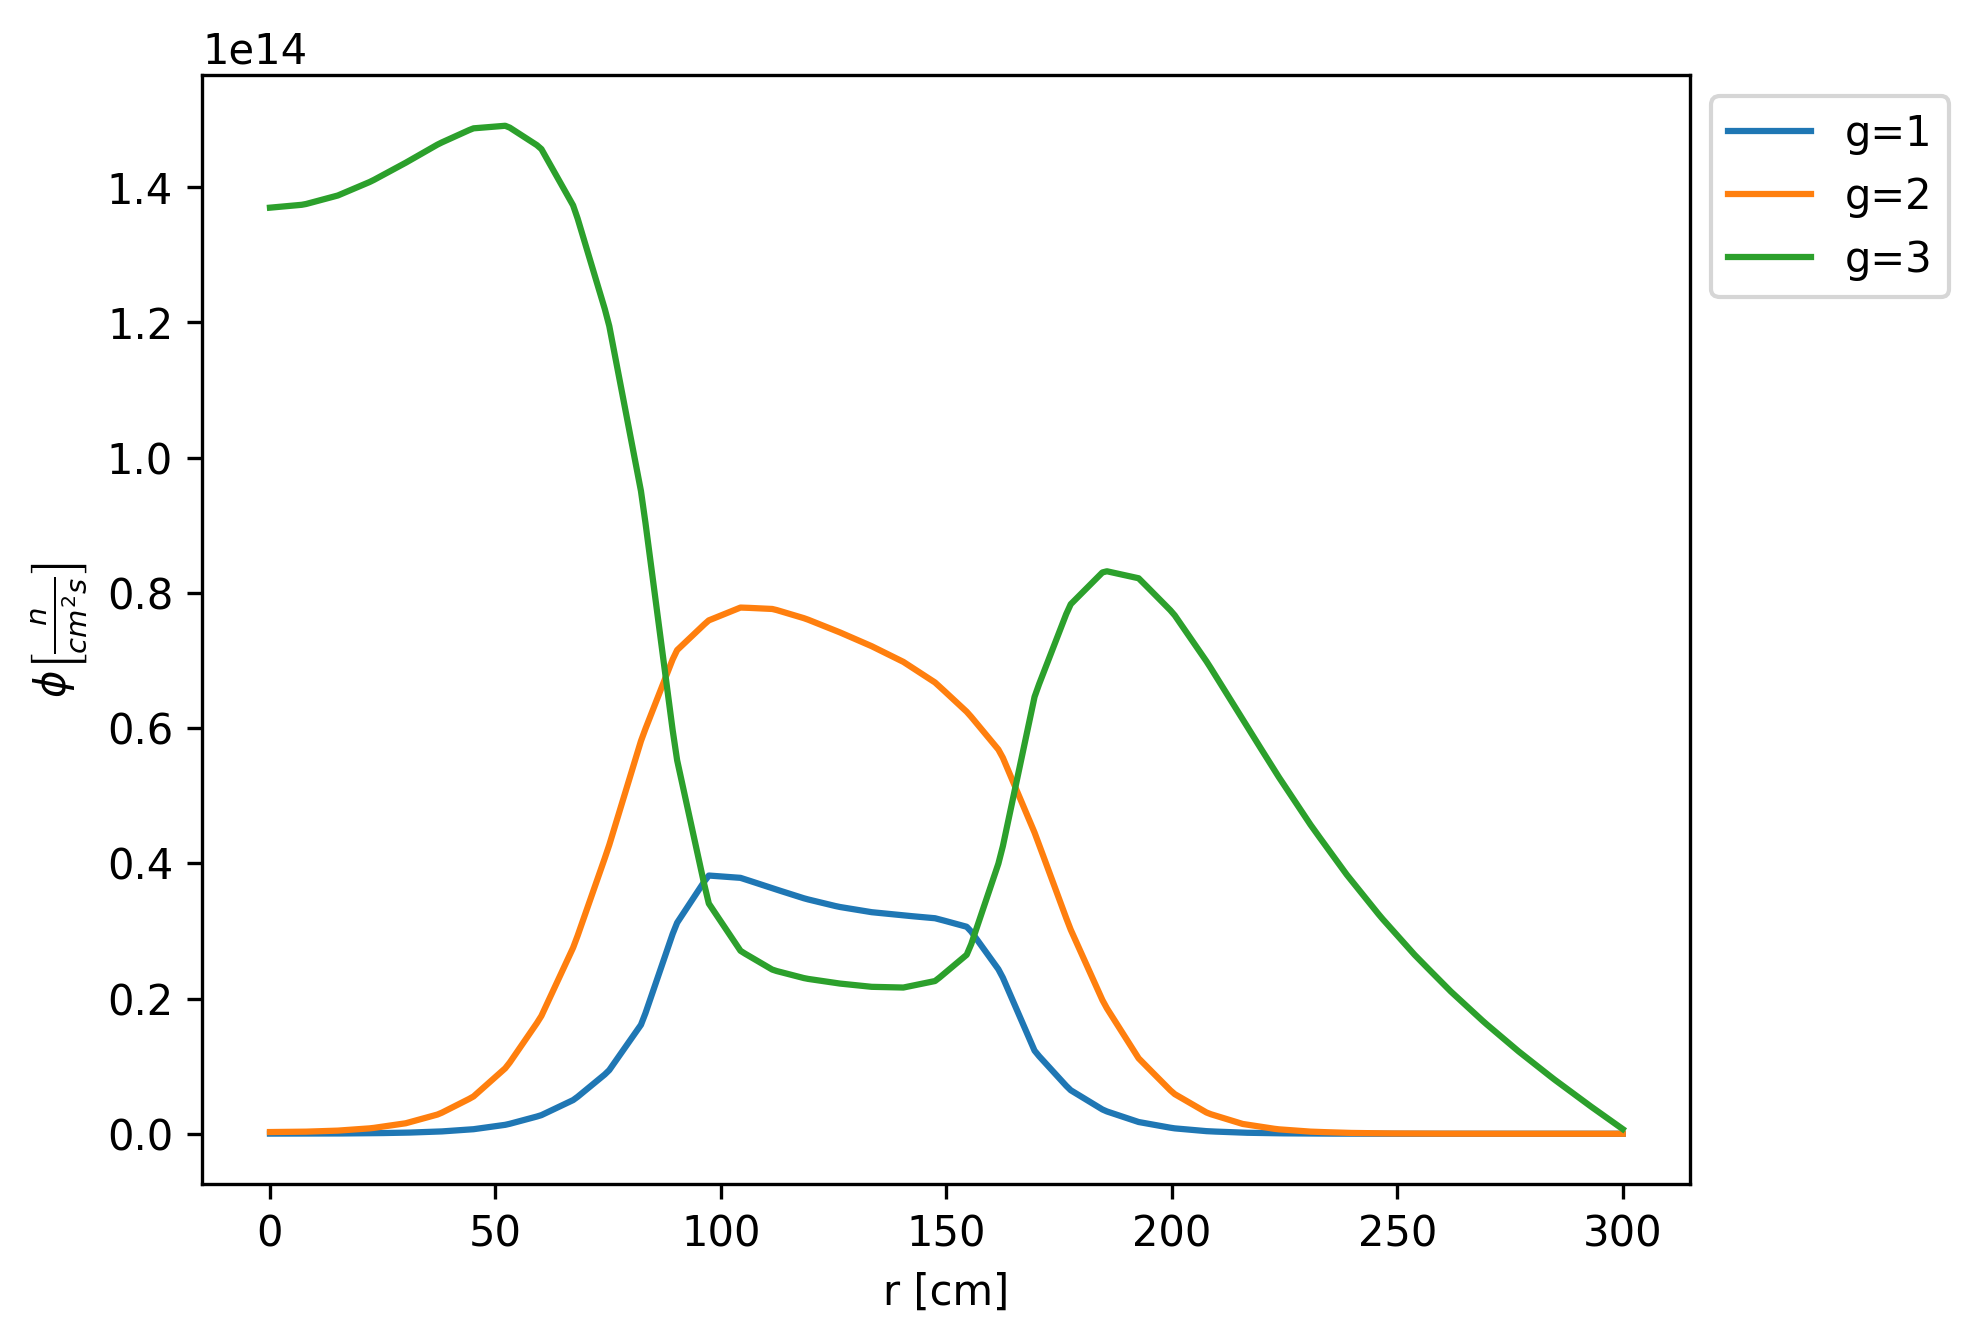
\includegraphics[width=\linewidth]{figures-fullcore/3D-fullcore-600-15Gd-radial1}
		\caption{Moltres.}
	\end{subfigure}
	\begin{subfigure}[t]{0.4\textwidth}
		\centering
		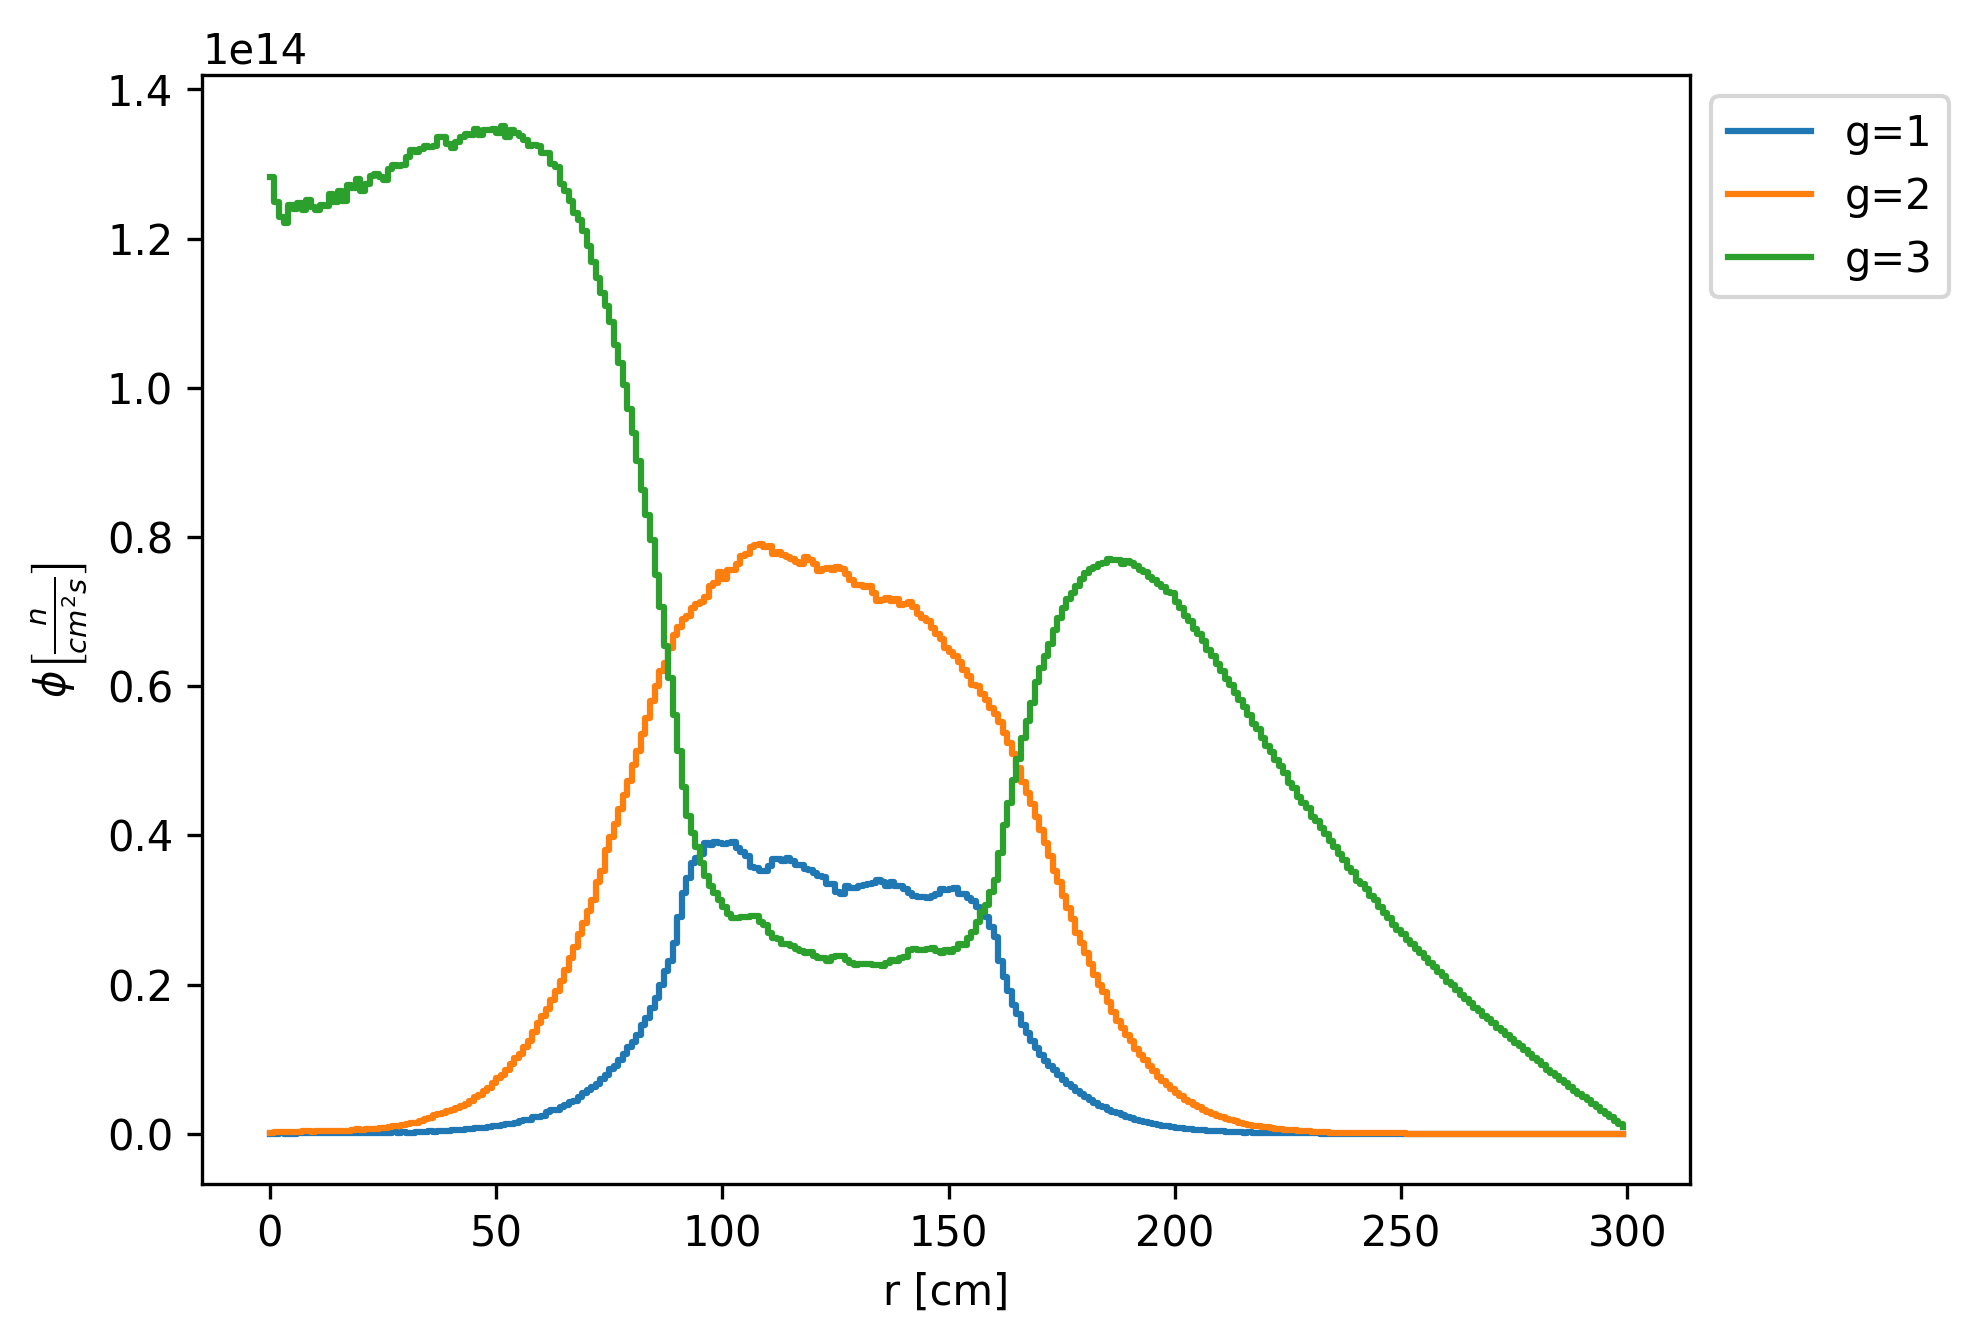
\includegraphics[width=\linewidth]{figures-fullcore/serpent26G-600-collapse-Radial}
		\caption{Serpent.}
	\end{subfigure}
	\hfill
	\caption{Radial flux at 600 K.}
	\label{fig:fullcore-600-radial1}
\end{figure}

%Axial flux1 at 1200K
\begin{figure}[htbp!]
	\centering
	\begin{subfigure}[t]{0.4\textwidth}
		\centering
		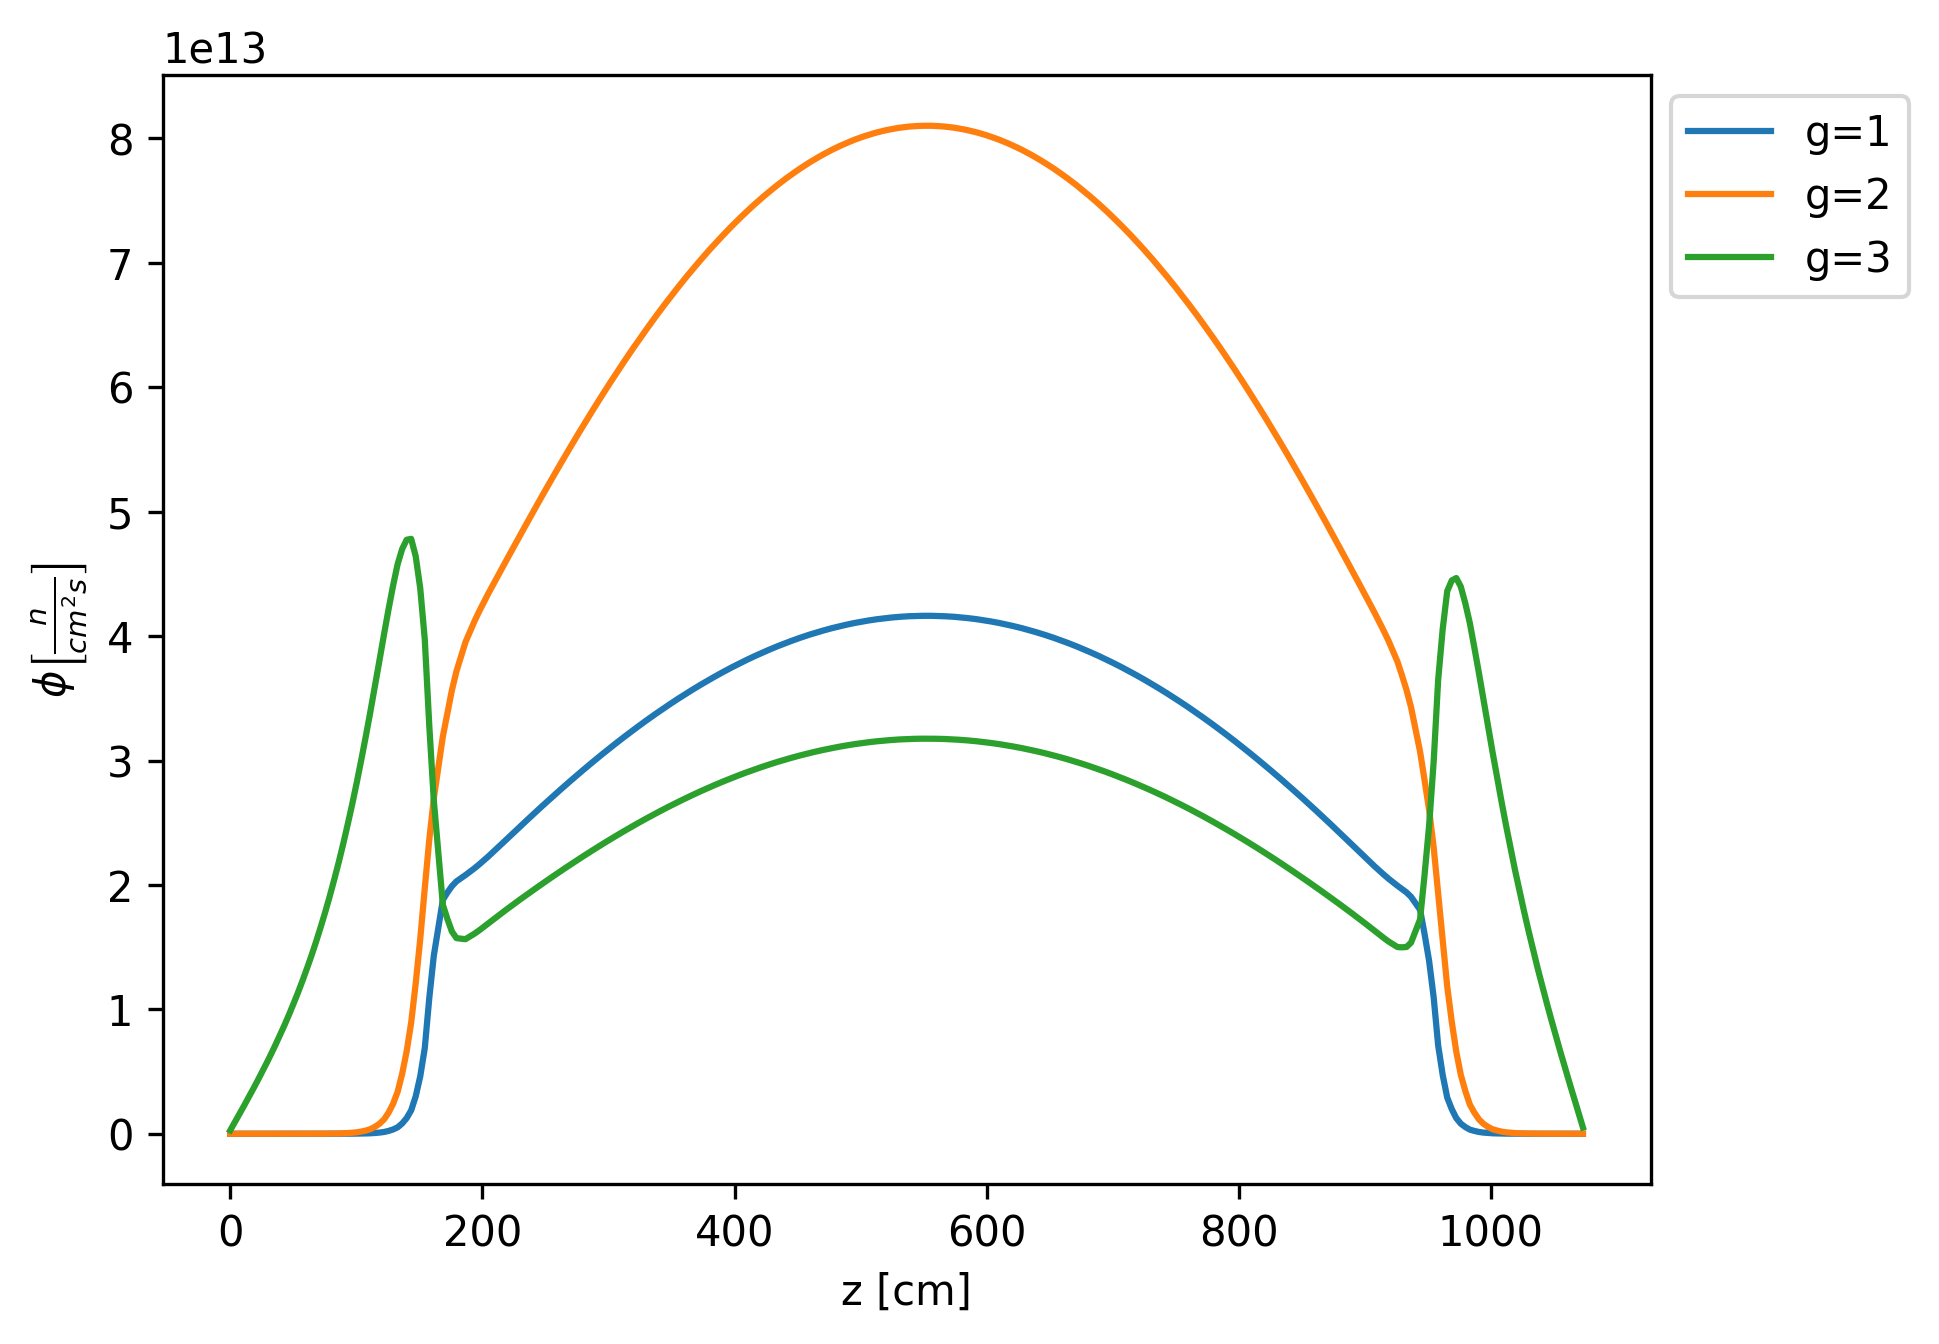
\includegraphics[width=\linewidth]{figures-fullcore/3D-fullcore-1200-15Gc-axial1}
		\caption{Moltres.}
	\end{subfigure}
	\begin{subfigure}[t]{0.4\textwidth}
		\centering
		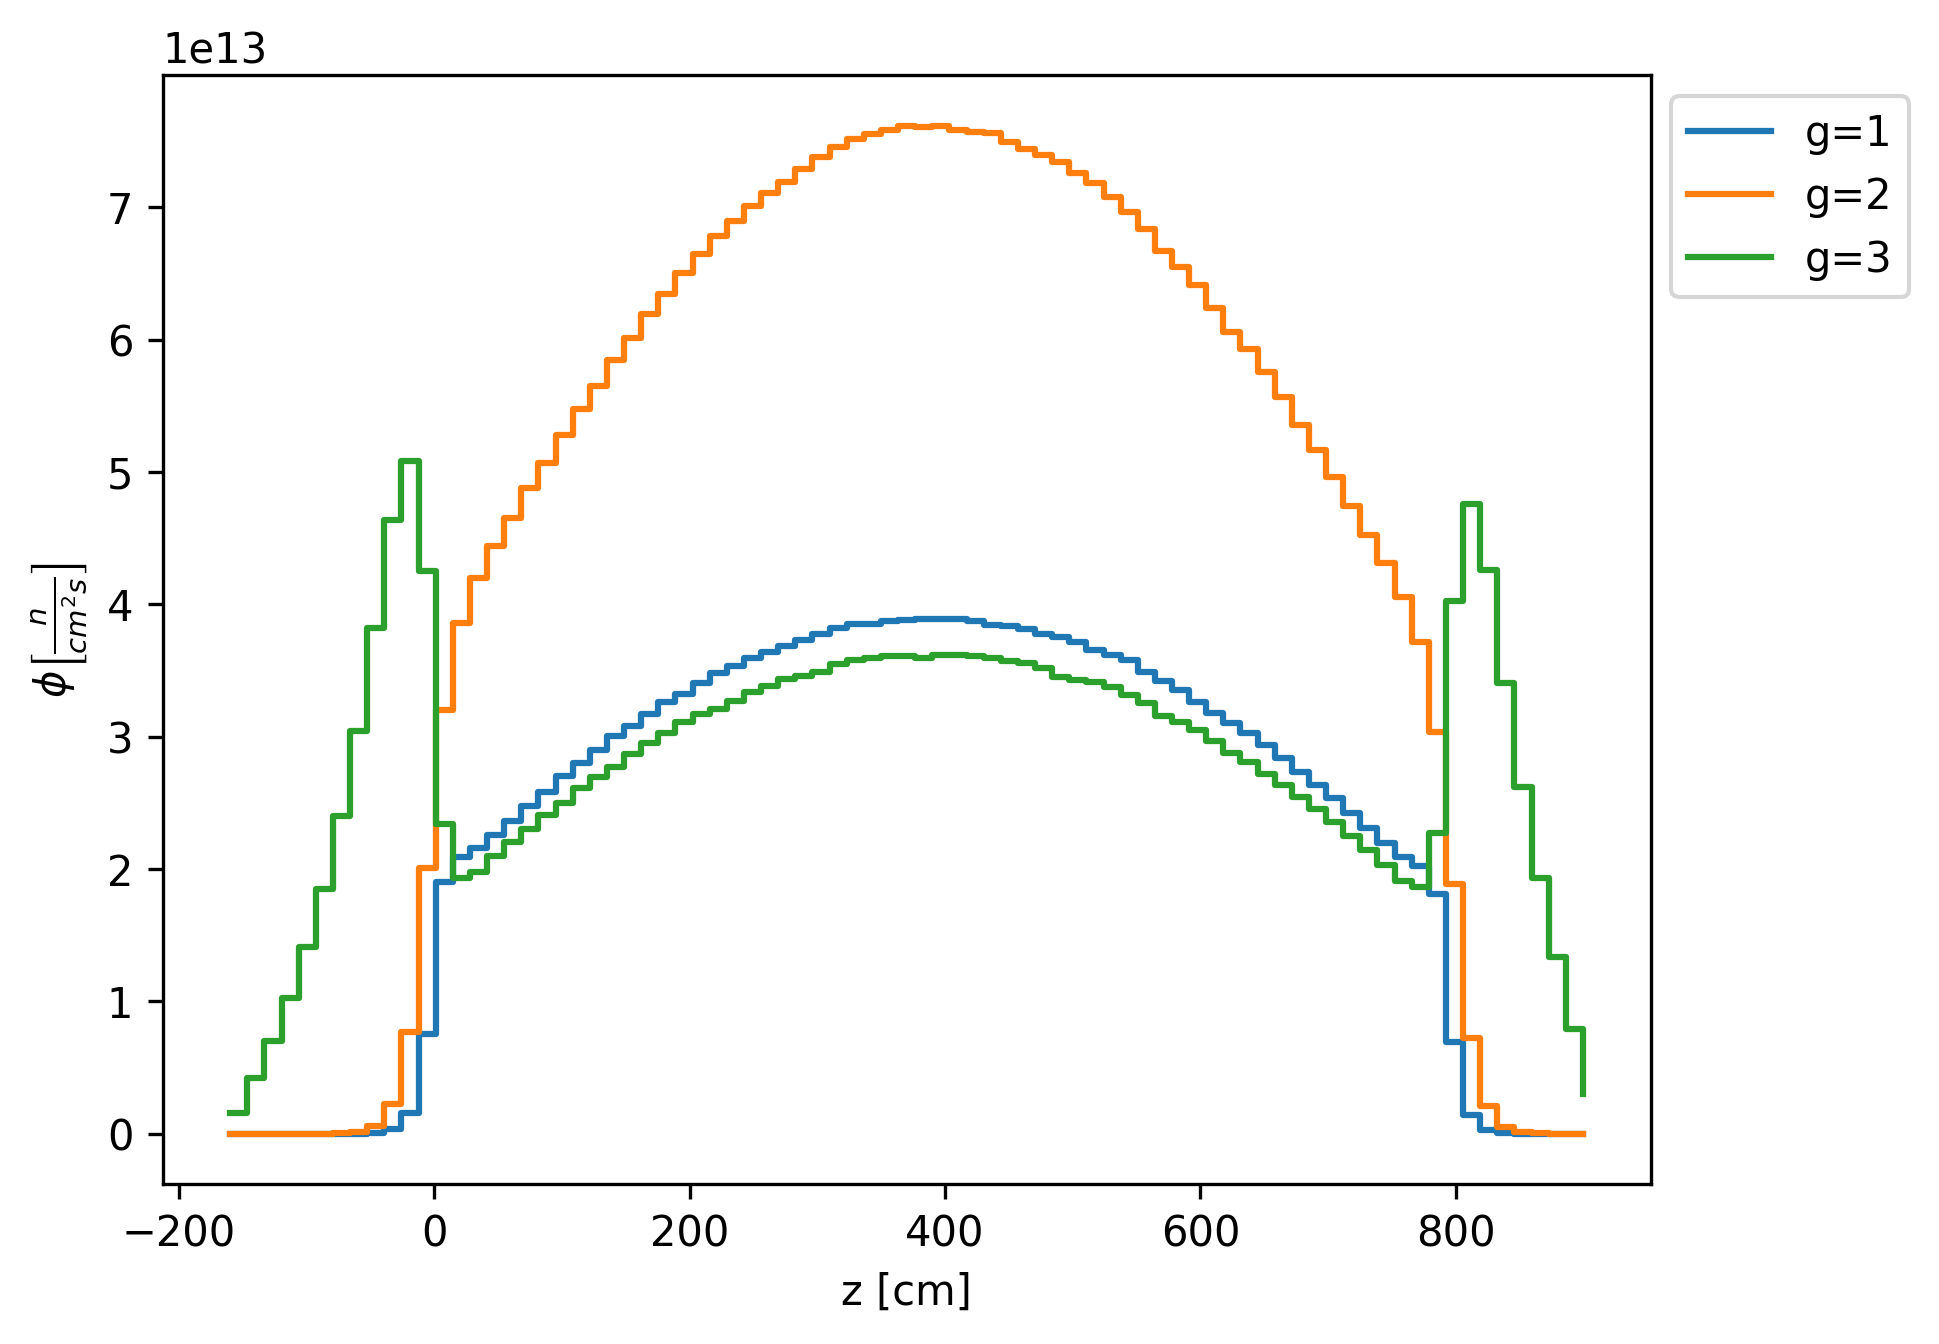
\includegraphics[width=\linewidth]{figures-fullcore/serpent26G-1200-collapse-Axial1}
		\caption{Serpent.}
	\end{subfigure}
	\hfill
	\caption{Flux in axial detector 1 at 1200 K.}
	\label{fig:fullcore-1200-axial1}
\end{figure}

%Axial flux3
\begin{figure}[htbp!]
	\centering
	\begin{subfigure}[t]{0.4\textwidth}
		\centering
		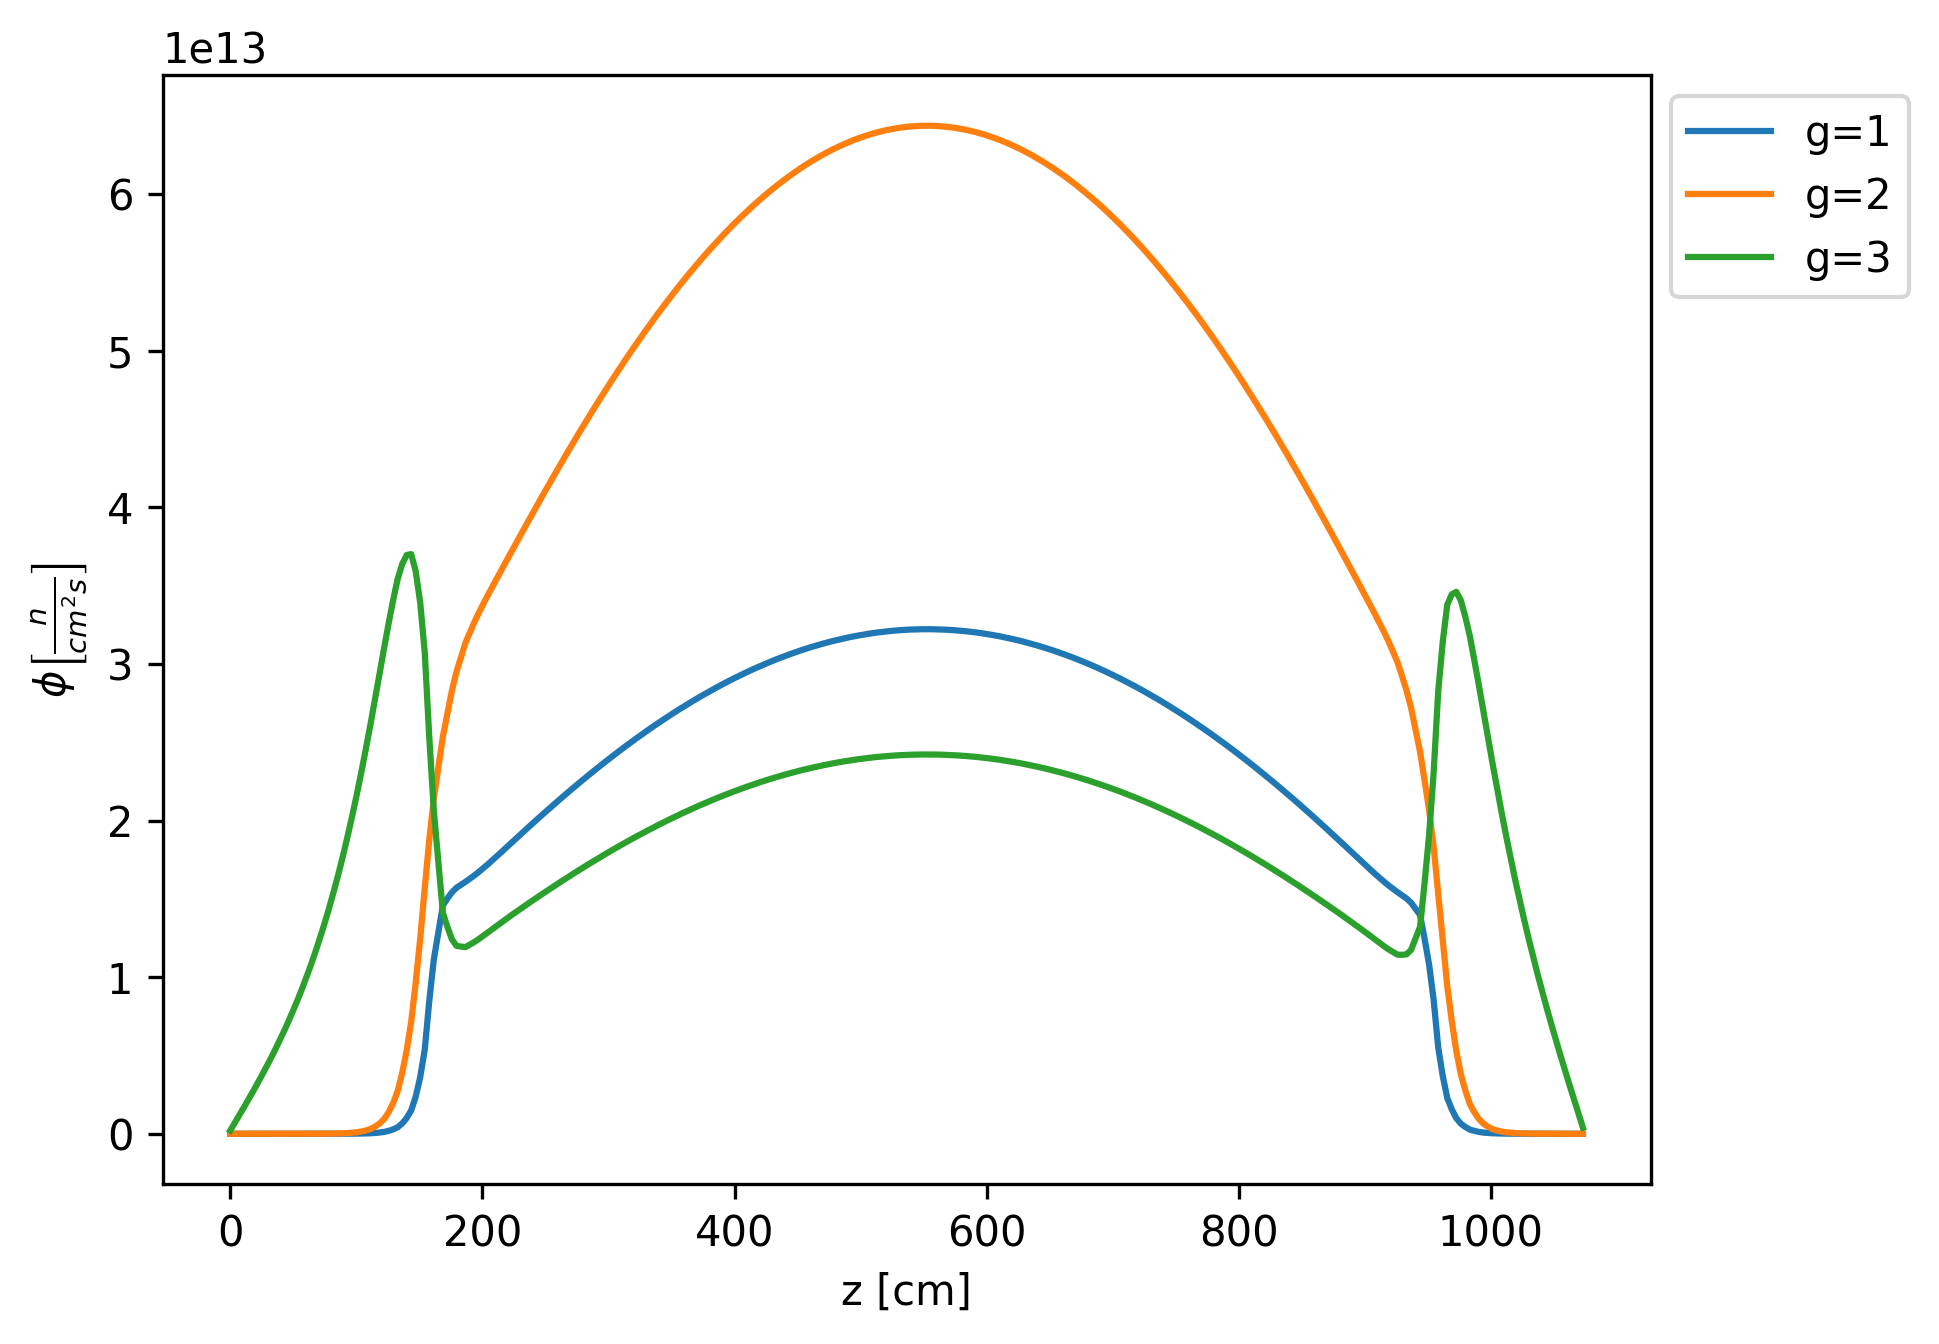
\includegraphics[width=\linewidth]{figures-fullcore/3D-fullcore-1200-15Gc-axial3}
		\caption{Moltres.}
	\end{subfigure}
	\begin{subfigure}[t]{0.4\textwidth}
		\centering
		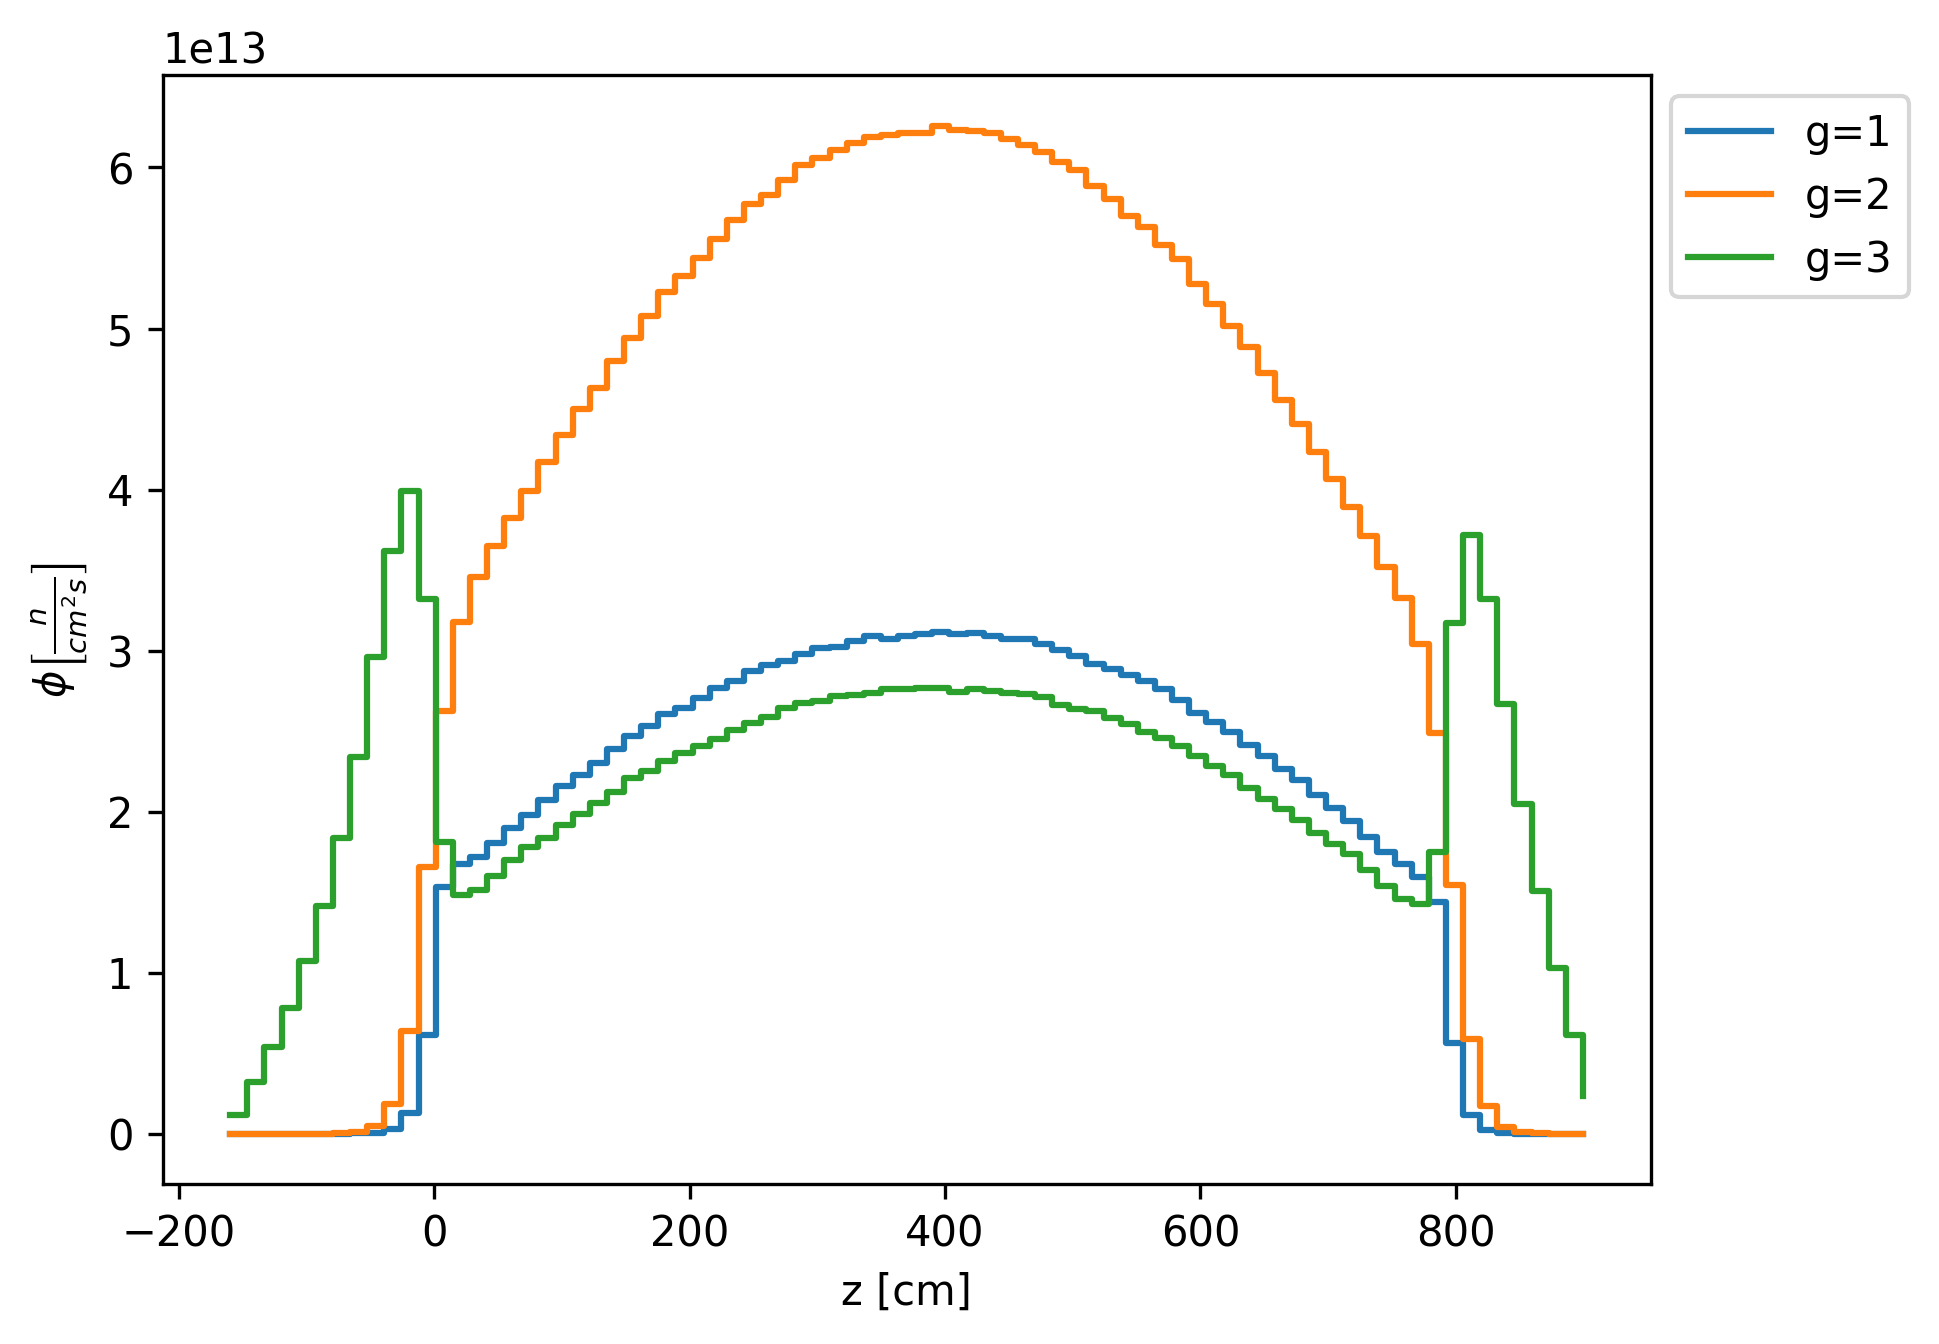
\includegraphics[width=\linewidth]{figures-fullcore/serpent26G-1200-collapse-Axial2}
		\caption{Serpent.}
	\end{subfigure}
	\hfill
	\caption{Flux in axial detector 2 at 1200 K.}
	\label{fig:fullcore-1200-axial2}
\end{figure}

%Radial flux
\begin{figure}[htbp!]
	\centering
	\begin{subfigure}[t]{0.4\textwidth}
		\centering
		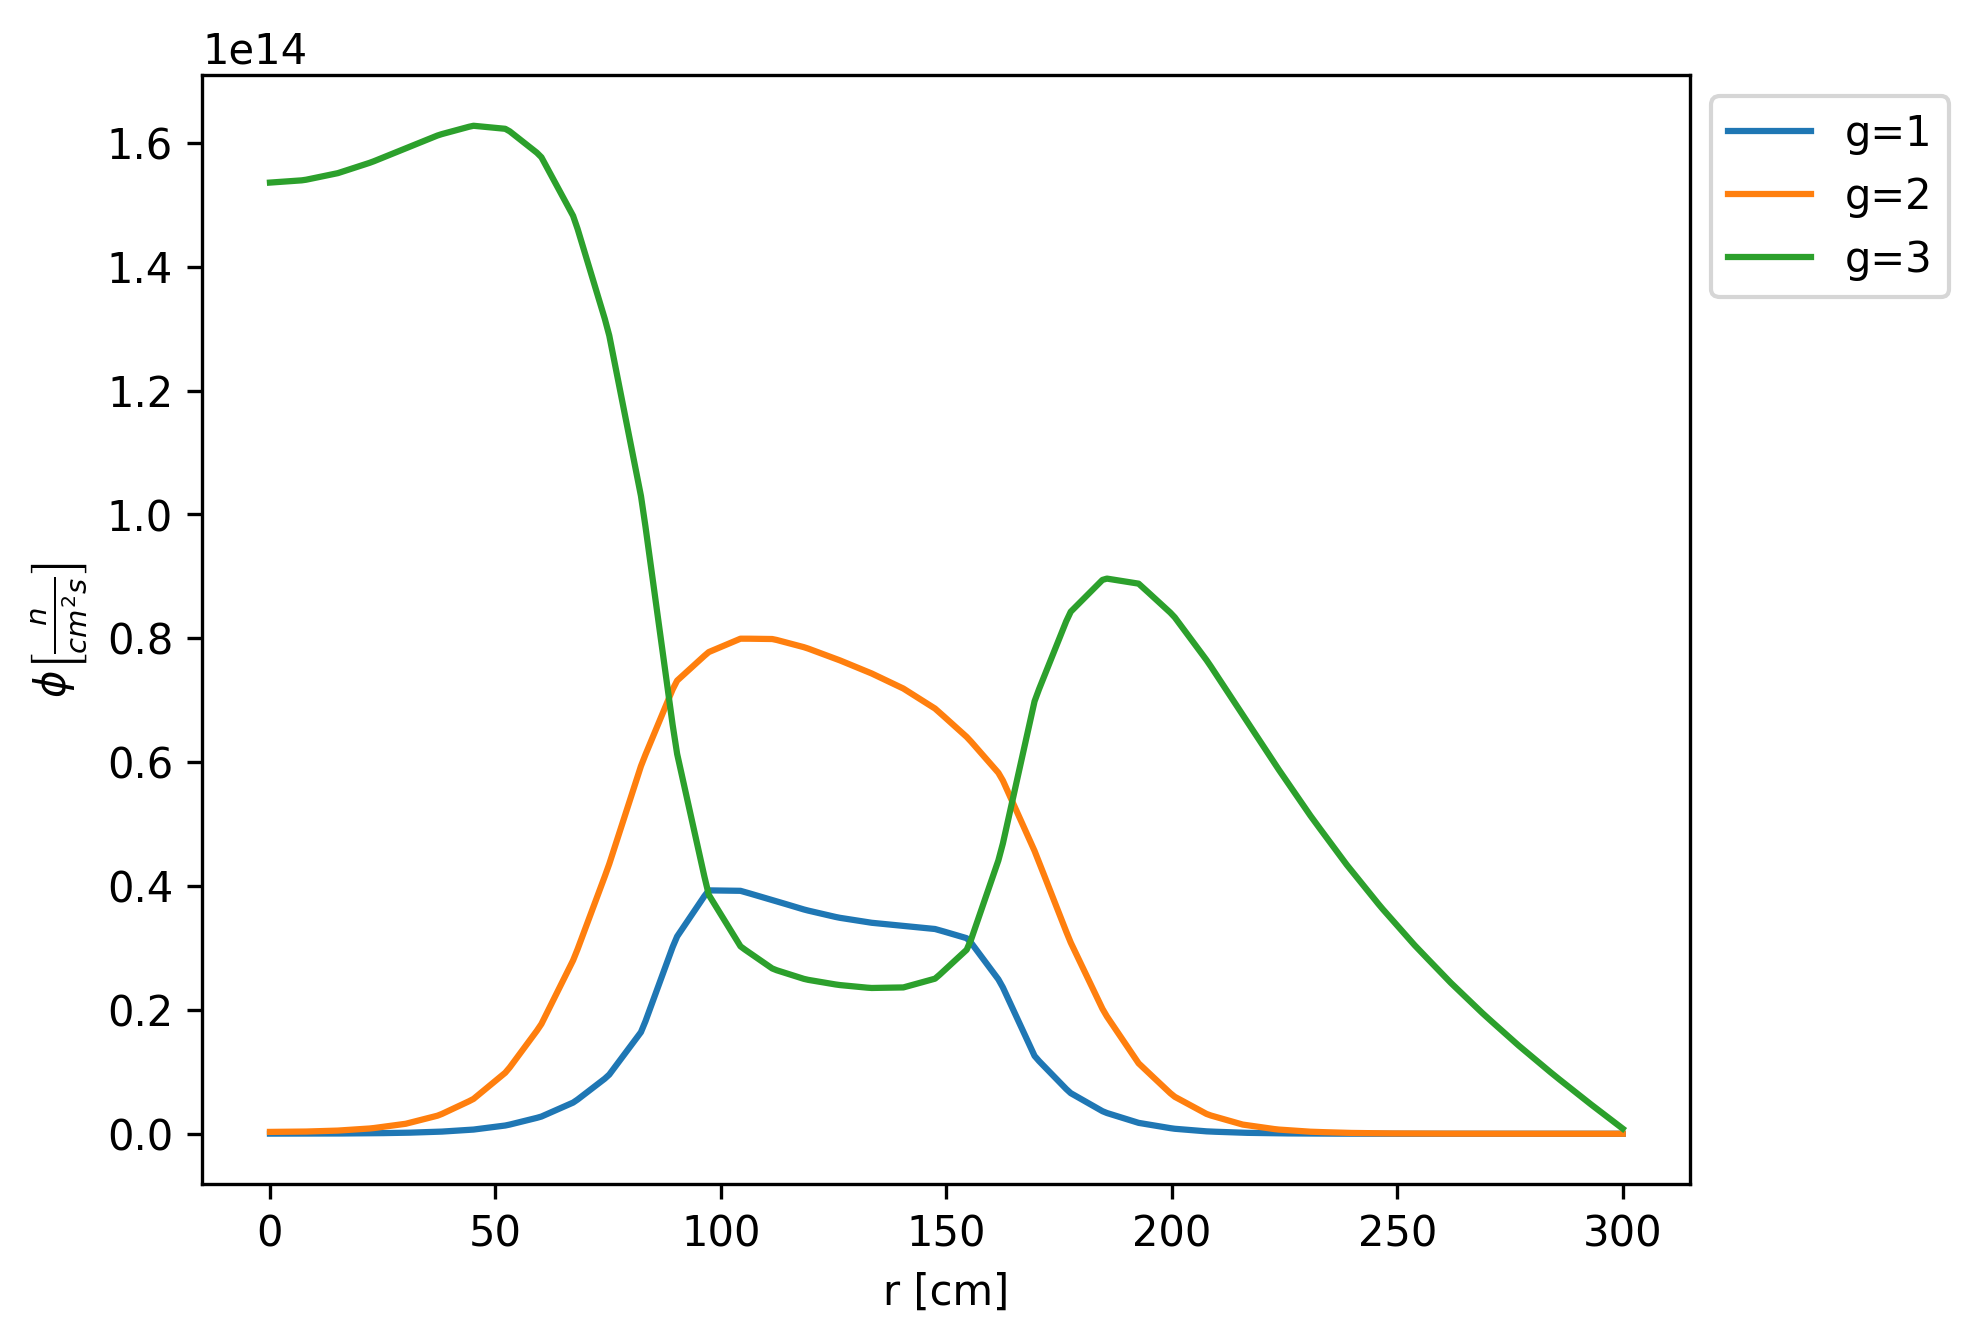
\includegraphics[width=\linewidth]{figures-fullcore/3D-fullcore-1200-15Gc-radial1}
		\caption{Moltres.}
	\end{subfigure}
	\begin{subfigure}[t]{0.4\textwidth}
		\centering
		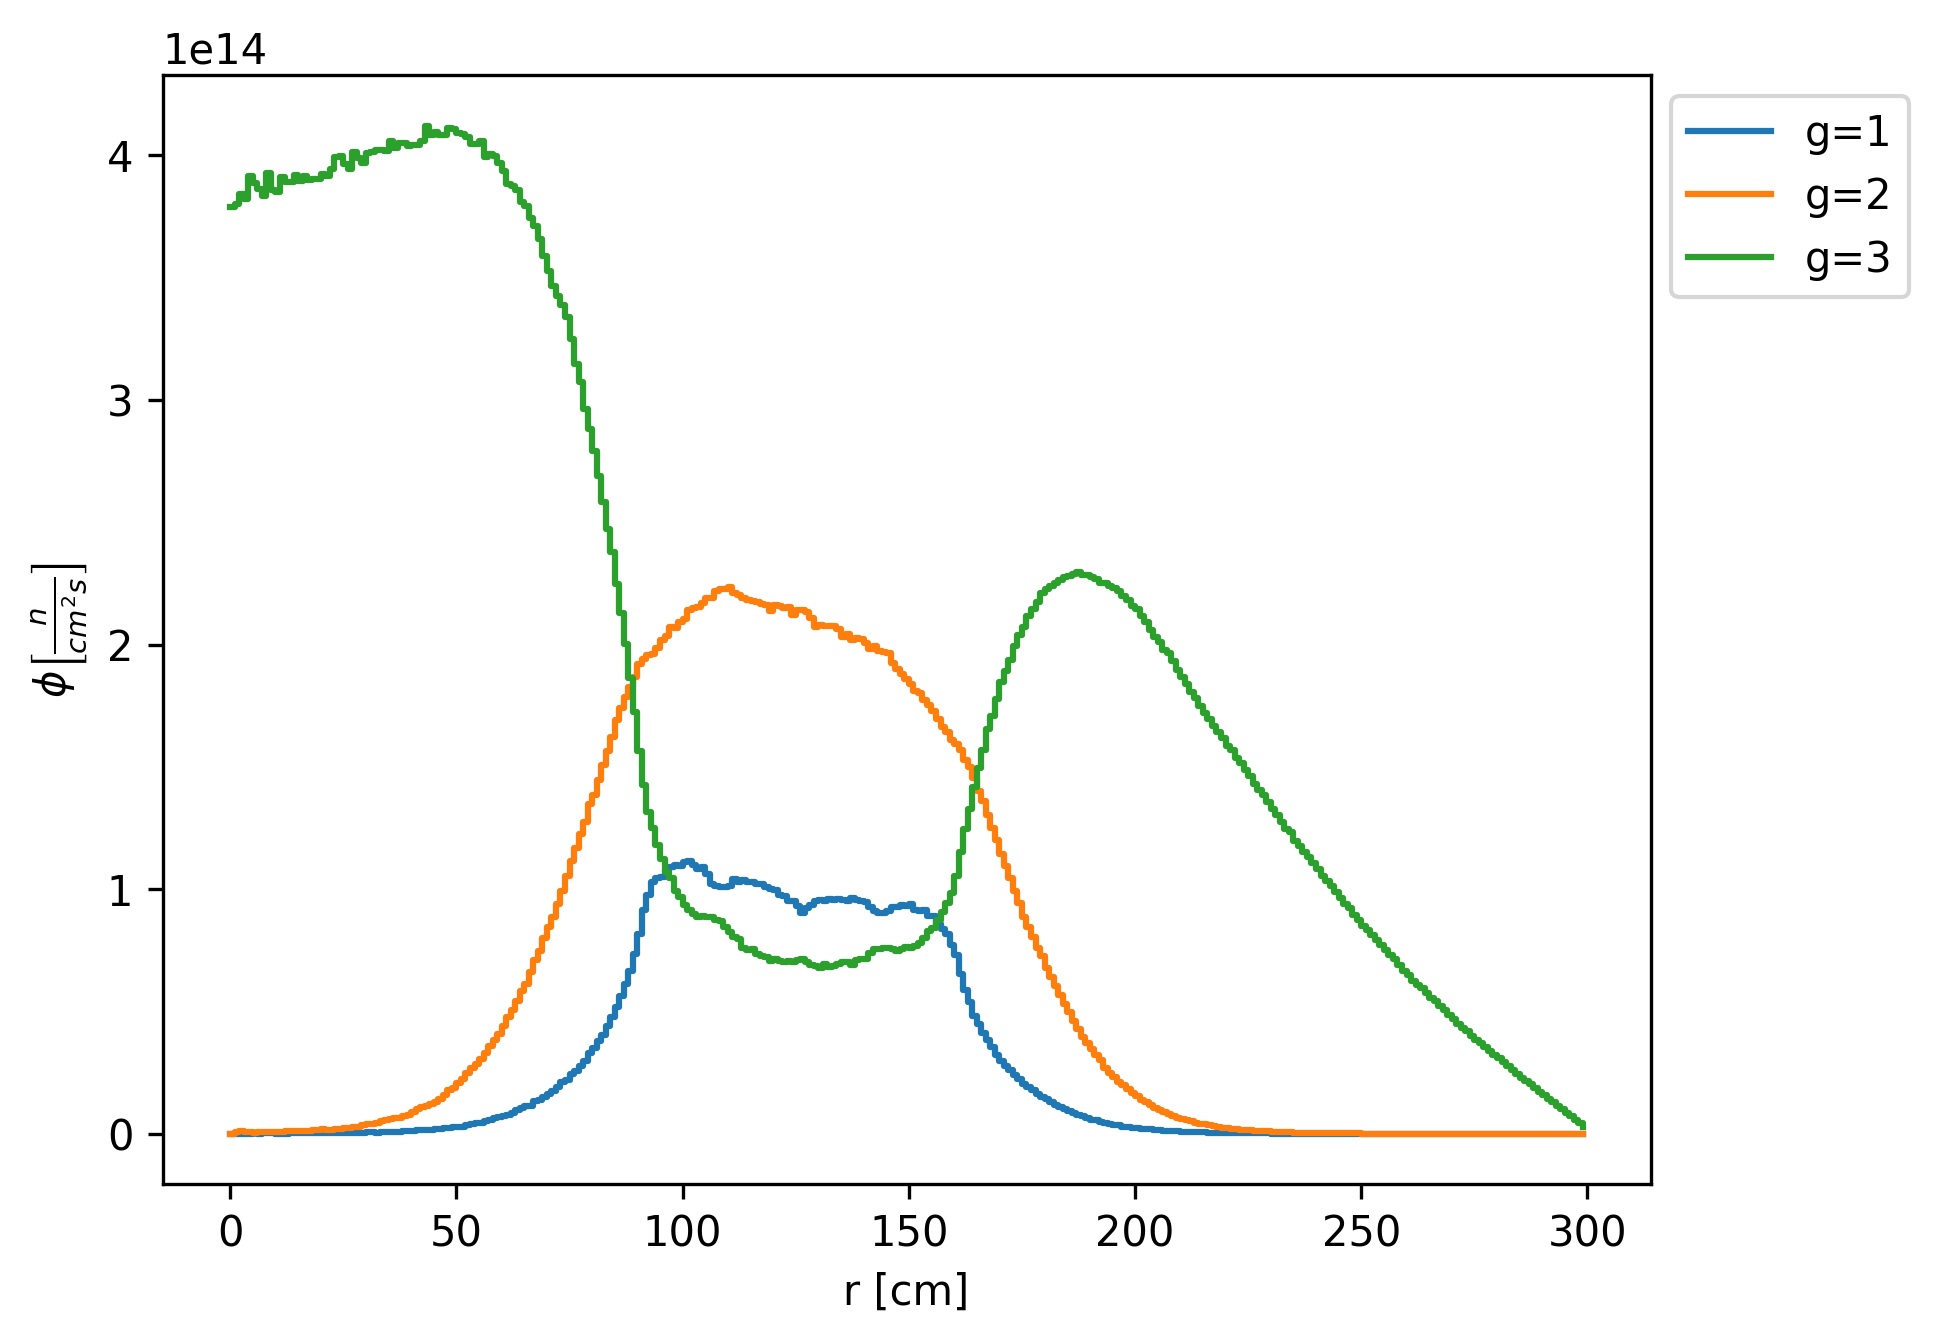
\includegraphics[width=\linewidth]{figures-fullcore/serpent26G-1200-collapse-Radial}
		\caption{Serpent.}
	\end{subfigure}
	\hfill
	\caption{Radial flux at 1200 K.}
	\label{fig:fullcore-1200-radial1}
\end{figure}

\pagebreak
\bibliographystyle{plain}
\bibliography{bibliography}

\end{document}

	% \begin{figure}[htbp!]
	% 	\centering
	% 	\begin{subfigure}[t]{0.4\textwidth}
	% 		\centering
	% 		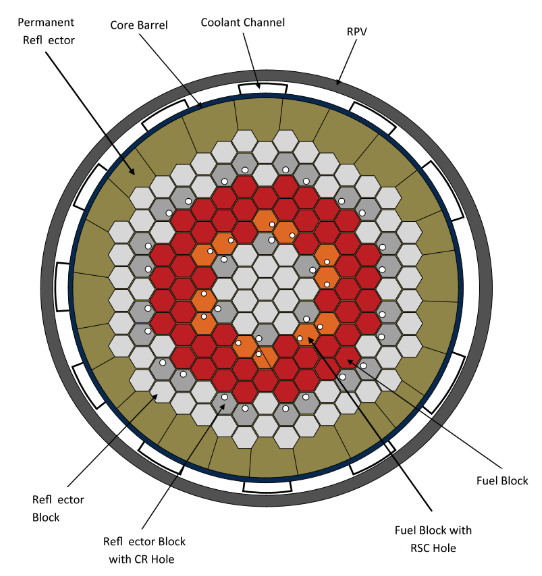
\includegraphics[width=\linewidth]{figures/radial-layout.png}
	% 		\caption{XY-plane.}
	% 	\end{subfigure}
	% 	\begin{subfigure}[t]{0.4\textwidth}
	% 		\centering
	% 		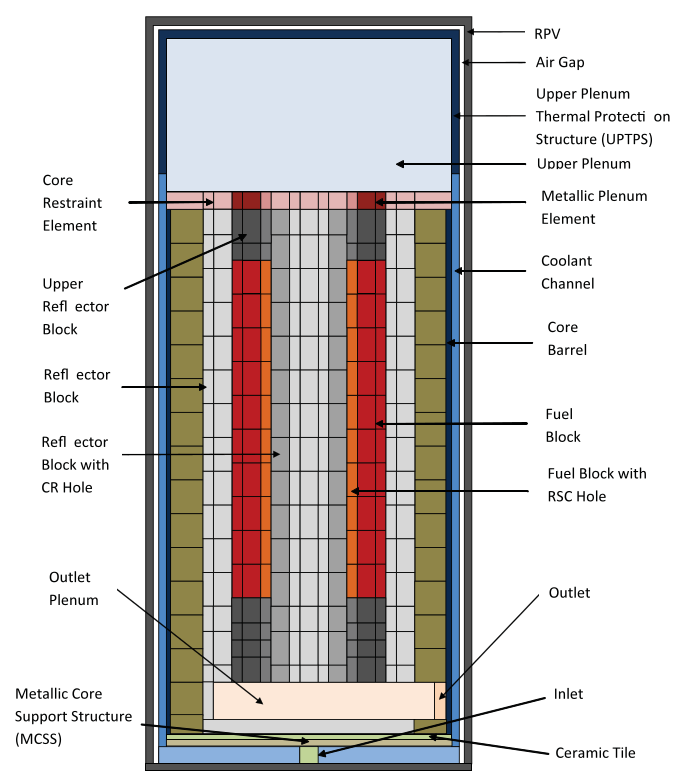
\includegraphics[width=\linewidth]{figures/axial-layout.png}
	% 		\caption{YZ-plane.}
	% 	\end{subfigure}
	% 	\hfill
	% 	\caption{MHTGR reactor layout.}
	% 	\label{fig:layout}
	% \end{figure}

	% \begin{figure}[htbp!]
	% 	\centering
	% 	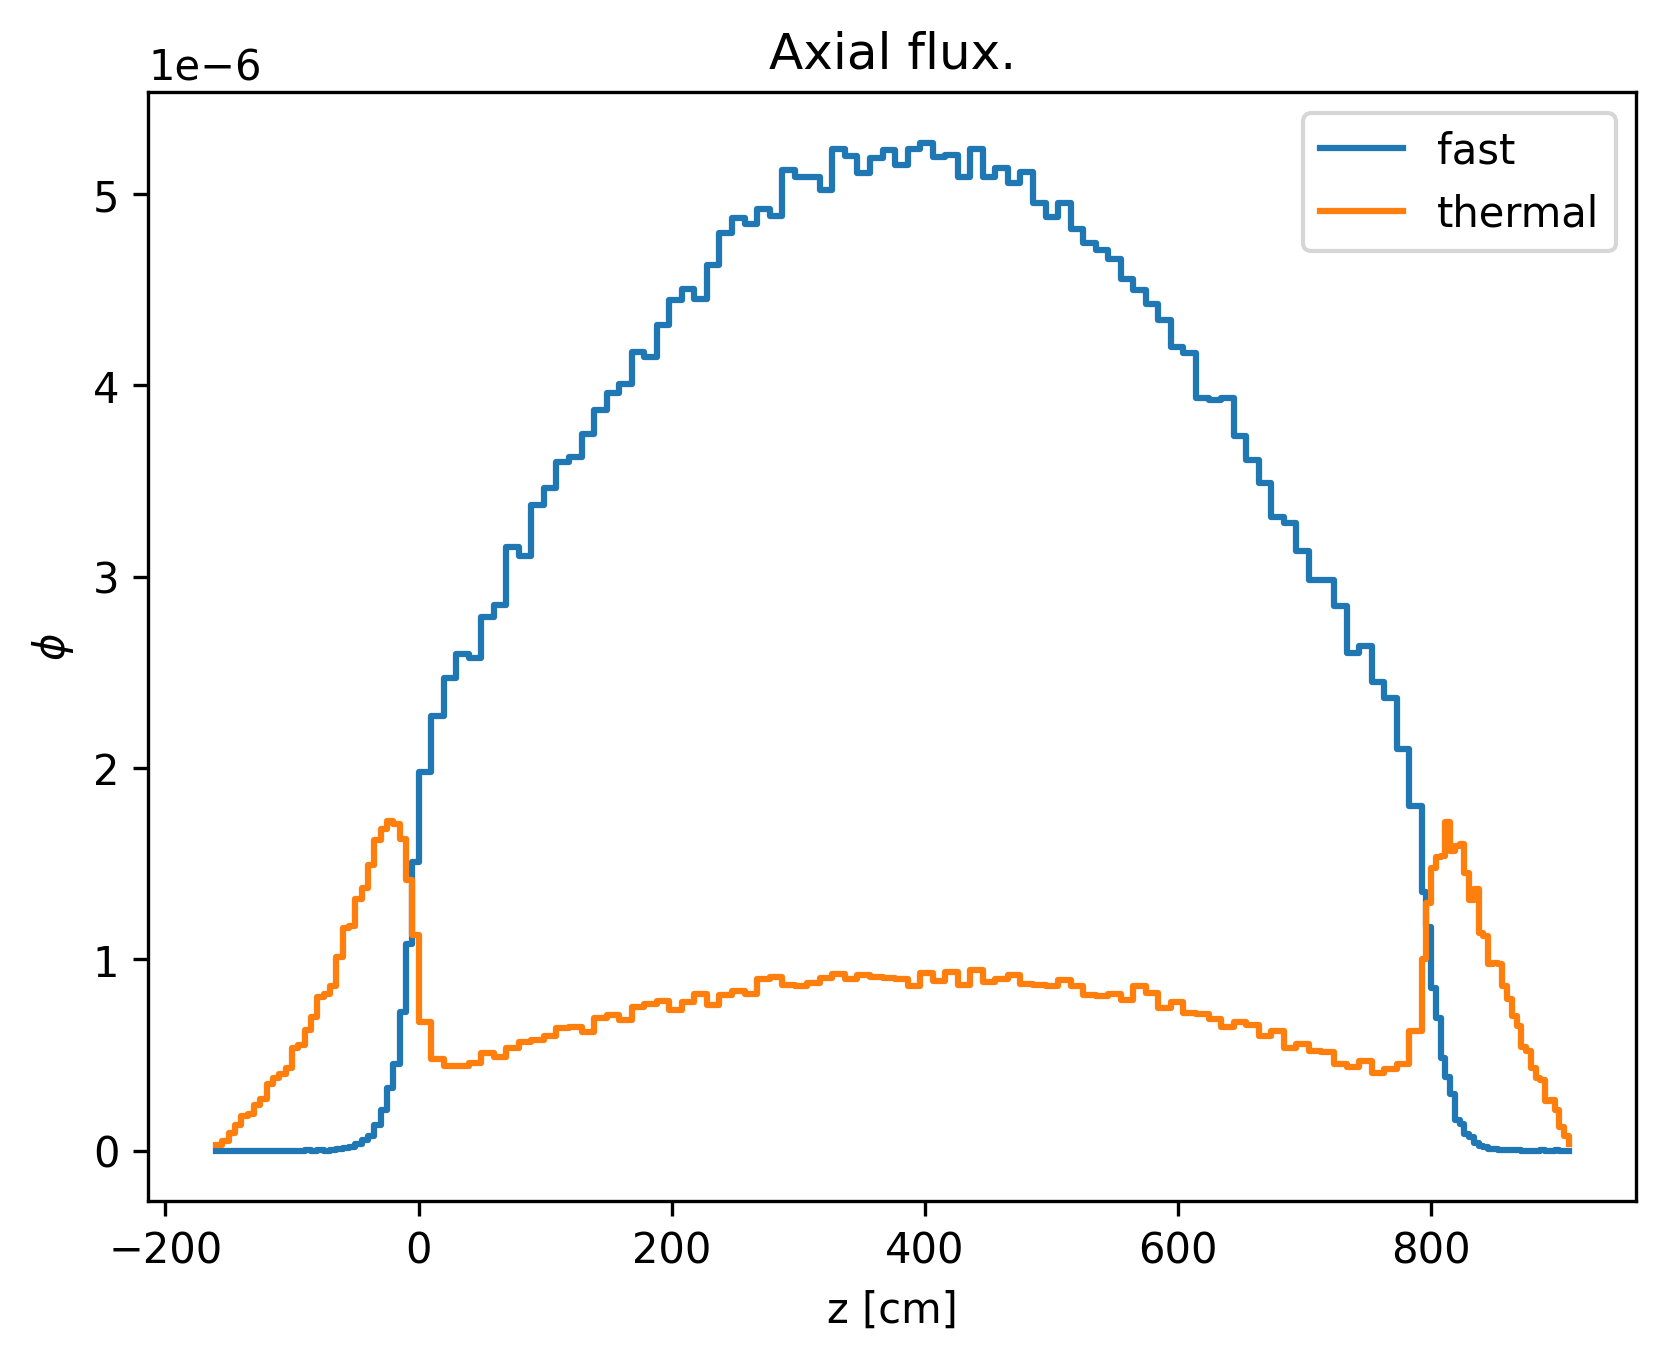
\includegraphics[width=0.6\linewidth]{figures/axial1.png}
	% 	\hfill
	% 	\caption{Neutron flux on the specified fuel channel.}
	% 	\label{fig:axial}
	% \end{figure}
